
%TODO: Find out what's different about ns-proposal used in reliability proposal
% \documentclass[letterpaper,10pt]{article}
%% \documentclass[10pt,onecolumn]{article}
\documentclass[10pt,onecolumn]{ns-article}
% \newcommand{\mydriver}{pdflatex}
% \documentclass[12pt,\mydriver]{thesis-2}
%% \usepackage[letterpaper, margin=1.25in]{geometry} % For giving to neil


\PassOptionsToPackage{hyphens}{url}
\usepackage[hyphens]{url}
\usepackage{hyperref}
\hypersetup{breaklinks=true}
\urlstyle{same}
\usepackage{balance}

% TODO: I seem to have used most of these from the reliability
% proposal. Find out what the role of each command is.
\usepackage{ifpdf,floatrow} 

% nspring 10.35pt palatino
\renewcommand*{\rmdefault}{ppl} % Roman default
\usepackage{fix-cm}
% \renewcommand{\normalsize}{\fontsize{10.35pt}{12.5pt}\selectfont}
% \renewcommand{\normalsize}{\fontsize{10pt}{12.5pt}\selectfont}
% endspring

%% ns - replacement for times that lacks stupidity.
% \usepackage{mathptmx}
% \usepackage[scaled=.90]{helvet}
% \usepackage{courier}
% 
% \usepackage[override]{cmtt} % make tt font tighter / less ugly

% \usepackage{makeidx}  % allows for indexgeneration

\usepackage[square,comma,numbers,sort&compress]{natbib}

\usepackage{titlesec}
   \titleformat{\chapter}
      {\normalfont\large}{Chapter \thechapter:}{1em}{}

\usepackage{color}
\usepackage[table]{xcolor}
\definecolor{orange}{RGB}{255,127,0}
\newcommand{\rama}[1]{{\color{red}[\todo{rama: #1}]}}
\newcommand{\ns}[1]{{\color{green}[ns: #1]}}
\newcommand{\etal}{et~al.\xspace}
\providecommand{\ie}{\emph{i.e.,} }
\providecommand{\eg}{\emph{e.g.,} }
\providecommand{\cf}{\emph{cf.,} }
\providecommand{\vs}{\emph{vs.} }
\providecommand{\etc}{\emph{etc.}}   
\providecommand{\ione}{\emph{(i)} }
\providecommand{\itwo}{\emph{(ii)} }
\providecommand{\ithree}{\emph{(iii)} }
\providecommand{\ifour}{\emph{(iv)} }
\providecommand{\ifive}{\emph{(v)} }

% \newcommand{\ignore}[1]{}

% Rk: The following commands came from the NSF reliability proposal
% \setlength{\textwidth}{6.5in}
% \setlength{\textheight}{9in}
% \setlength{\topmargin}{0in}
% \setlength{\headheight}{0in}
% \setlength\columnsep{.30in}
% \setlength{\headsep}{0in}
% \setlength{\oddsidemargin}{0pt}
% \setlength{\evensidemargin}{0pt}

% Rk: The following commands are from mainthesis.tex from UMD's
% official style guide. Revisit and fix to get tables.
% \newcommand{\tbsp}{\rule{0pt}{18pt}} %used to get a vertical distance after \hline
% \renewcommand{\baselinestretch}{2}
% \setlength{\textwidth}{5.9in}
% \setlength{\textheight}{9in}
% \setlength{\topmargin}{-.50in}
% %\setlength{\topmargin}{0in}    %use this setting if the printer makes the the top margin 1/2 inch instead of 1 inch
% \setlength{\oddsidemargin}{.55in}
% \setlength{\parindent}{.4in}
% \pagestyle{empty}

\setlength{\textfloatsep}{.1in plus 0.05in}
\setlength{\itemsep}{-10pt}


\usepackage{enumitem}
\setlist[itemize]{leftmargin=*}
% \usepackage{slashbox}
\usepackage{graphicx}
\usepackage{amsmath,amssymb}
\usepackage{verbatimbox}
\usepackage{boxedminipage}
\usepackage{multirow}
% \usepackage{subfigure}
\usepackage[labelformat=simple]{subcaption}
% \usepackage{subfig}
\usepackage{xspace}
\usepackage[]{pdfpages}

\usepackage[utf8x]{inputenc}
\usepackage{ucs}

% \newcounter{FileStack}
% \let\OrigInput\input
% \newcommand{\ninput}[1]{%
%   \stepcounter{FileStack}
%   \expandafter\let
%   \csname NameStack\theFileStack\endcsname
%   \ThisFile
%   \def\ThisFile{#1}%
%   \OrigInput{#1}%
%   \expandafter\let\expandafter
%   \ThisFile
%   \csname NameStack\theFileStack\endcsname
%   \addtocounter{FileStack}{-1}%
% }

%boxed,vlined,,linesnumbered,commentsnumbered
\usepackage[vlined]{algorithm2e}
\providecommand{\SetAlgoLined}{\SetLine}
\providecommand{\DontPrintSemicolon}{\dontprintsemicolon}





\newcommand{\planetlab}{PlanetLab\xspace}

\renewcommand\thesubfigure{(\alph{subfigure})}

%\usepackage{algorithm}s}
\title{Analyzing Internet reliability remotely with probing-based techniques}
% \title{Thesis Proposal: Remote probing-based outage detection for
%   individual IP addresses}

\author{Ramakrishna Padmanabhan}

\begin{document}

% Define table specific commands
\newcommand{\bb}{~~~~~}
\newcommand{\hdr}[1]{\multicolumn{1}{c}{\textbf{#1}}}
% define ``struts'', as suggested by Claudio Beccari in
%    a piece in TeX and TUG News, Vol. 2, 1993.
\newcommand\Tstrut{\rule{0pt}{2.2ex}}         % = `top' strut
\newcommand\Bstrut{\rule[-0.9ex]{0pt}{0pt}}   % = `bottom' strut

\newcommand{\figdone}{} % \textcolor{blue}{FINAL}}

\maketitle


\begin{abstract}

% We use the Internet without know that the Internet is actually super reliable. It's based more upon: hey, the Internet seems reliable. 

% The Internet is used today for communication

% Detection of Internet outages, which are potentially rare events, demands broad and longitudinal measurements of users' Internet connections.
% Internet reliability is increasingly important as the applications we use increasingly depend upon the Internet.
% Internet reliability is increasingly important as a variety of services that we use migrate to the Internet.
% Internet reliability is increasingly important as the applications that we depend upon migrate to the Internet.
Internet reliability is increasingly important as a variety of services that we use migrate to the Internet. Yet, we lack authoritative measures of last-mile Internet reliability. The first step towards measuring last-mile reliability is to detect Internet outage events experienced by users. Since Internet outages are rare events, detecting them requires broad and longitudinal measurements; however, such measurements of Internet reliability at the individual user level are challenging to obtain accurately and at scale. The second step is to use detected outages to reason about Internet reliability across different dimensions such as ISPs, media-types, and geographical areas.

Probing-based remote outage detection techniques can scale but their accuracy is questionable. These techniques detect Internet outages across time as well as across the IPv4 address space by sending active probes, such as pings and traceroutes, to users' IP addresses and use probe responses to infer Internet connectivity. However, they can infer false outages since their foundational assumption can sometimes be invalid: that the lack of response to an active probe is indicative of failure. I illustrate two potential scenarios where this assumption is invalid. In the first scenario, responses are delayed beyond the prober's timeout, leading these techniques to infer packet-loss instead of delay. In the second scenario, these techniques can falsely infer packet-loss when the address they are probing gets dynamically reassigned. I examine how commonly delayed responses and dynamic reassignment occur across ISPs to quantify the inaccuracy of these techniques. 

Next, I demonstrate how detected outages can be used to perform meaningful assessments of Internet reliability. One aspect of Internet reliability is the study of how an external factor (like the occurence of thunderstorms) affects Internet connectivity; I show how to study the effect of such a factor upon the reliability of a group of addresses by studying the \emph{inflation} in outage rate for that group during its presence. Measuring the inflation in outage rate mitigates the effects of false outages. I also develop and evaluate an approach to segregate outages into categories that suggest their cause. Outages could result from a variety of causes, such as power outages, voluntary shutdown of users' home Internet equipment, network outages due to an ISP's infrastructure failure etc. When assessing the reliability of a particular ISP, we would ideally consider only the subset of outages that affect solely that ISP. I propose a technique to segregate outages by detecting simultaneous outages of ``related'' groups of addresses (addresses may be related by geography, ISP, or network topology). Simultaneous outages can serve as evidence that a detected outage affected multiple users in a particular ISP.

Implementing these proposed techniques will help achieve comprehensive measurements of Internet reliability that can be used to identify vulnerable networks and their challenges, inform which enhancements can help networks improve reliability, and evaluate the efficacy of deployed enhancements over time.

% comprehensive datasets of Internet reliability that can aid in improving reliability by targeting problem regions or adapting strategies that have proven to be successful
\end{abstract}

\newpage


% \section{Preliminaries}

\section{Introduction}


% With online accessibility of
% devices ranging from temperature control systems to baby monitors in
% this Internet of Things era, our dependence upon the Internet for
% increasingly many facets of our daily lives only continues to
% rise.

% With the ability to access a
% variety of devices online in this Internet of Things era, ranging from
% temperature control systems to baby monitors, our dependence upon the
% Internet for increasingly many facets of our daily lives only
% continues to rise. 

% As the range of Internet services that we rely upon increases, so does our reliance upon
% the Internet. 

% Talk more about how important the Internet is?

Residential Internet reliability is increasingly important as a variety of
services that we use migrate to the Internet. Internet users today can
communicate with each other, perform financial transactions, plan
their travel, and even obtain critical services such as health
monitoring~\cite{ideal-life, remote-health-elderly} and emergency
services~\cite{emergency-voip-voipfone, emergency-voip-fcc} from their
homes. Our dependence upon the Internet will rise further as more of
our home devices become connected in this Internet of Things
era. Consequently, continuous availability of the Internet and
resilience is vital, and the reliability of the Internet is of
interest to stakeholders across the board, from government regulators and
Internet Service Providers, to users.

% TODO: How do I connect the next sentence neatly to the previous
% paragraphs? Especially when the previous paragraphs will go on to
% talk about all the interested parties at length.

% TODO: Look into billionts for citations about regulator interest.

Broad and longitudinal
measurements of users' Internet reliability in different circumstances
can identify vulnerable networks and their challenges, can inform
which enhancements can help these networks improve reliability, and
can evaluate the efficacy of deployed enhancements.

% Measuring
% Internet reliability at the individual user level will therefore prove invaluable in assessing
% the current state of Internet connectivity and in developing future
% enhancements.

% By detecting outage events and their duration, we
% can reason about a particular user's Internet reliability and compare
% it to other users' reliability across geography, ISPs, and
% media-types.

% Talk about how Internet reliability is difficult and who is
% interested. FCC. Even ISPs (Cite the "Nevermind" paper by Nick
% Duffield which claims that ISPs are typically reactive and wait for
% customers to call). Common users.

Yet, we lack authoritative measures of last-mile Internet reliability. The first step towards measuring users' Internet
reliability is to detect \emph{Internet outages}---events that prevent
users from communicating over the Internet. Since we expect outage
events to be rare, detecting them requires broad and longitudinal
measurements of individual users. However, such measurements of
Internet reliability at the individual user level are challenging to
obtain accurately and at scale. The next step towards measuring users'
reliability is to segregate detected outages into categories
that suggest their cause. Once outages are categorized in this
manner, we can estimate the reliability of an ISP by considering the
subset of outages that affected solely that ISP.

Existing techniques that measure individual-user-level outages can be
grouped into on-premises outage detection techniques and remote probing-based
outage detection techinques. On-premises techniques, such as
RIPE Atlas~\cite{atlas}, SamKnows~\cite{samknows}, and
BISmark~\cite{bismark-main-bib}, measure diverse aspects of
users' Internet connections, but
measure relatively few users. These techniques 
deploy dedicated hardware at user premises that continuously conduct ping,
traceroute, DNS measurements etc.; some of these
measurements can be used to infer Internet connectivity problems. Whereas hardware
based techniques have fundamental scaling difficulties owing to
manufacturing and deployment costs, hundreds of millions of
IP addresses respond to active probes~\cite{timeouts}. Since many
residences have at least one device with a public IP address ~\cite{cgn-imc16}
(typically the home router), these IP addresses can be probed
remotely, from 
vantage points that we control, to measure their connectivity. Thunderping~\cite{pingin} and Trinocular~\cite{trinocular} adopt this
approach to outage detection, taking a
complementary approach to on-premises techniques: they focus upon
measuring only connectivity but do so for many users. Since these
techniques can send probes remotely from servers under their control, without requiring any user
involvement, they are able to detect outages across time
as well as across the IPv4 address space.
% However, existing techniques do
% not study latency and therefore do not identify performance
% degradation resulting from high delay.
However, probing-based remote outage detection techniques can
make false inferences about outages when some scenarios
occur~\cite{timeouts, addrchange-reasons}. Further, existing
techniques have not 
attempted to categorize detected outages by their likely cause.
% However, measuring residential
% outages is challenging because of the scale: there are millions of
% residential links to measure. 
% Second, users can voluntarily power
% down their home Internet equipment and it is challenging to
% distinguish between voluntary user shutdowns and an outage at the last-mile link.
 
% ; even multihomed last mile links for business connectivity
% often share the same upstream hardware, representing a single point of 
% failure~\cite{twcable-business-web}. 
% Last-mile links lack the redundancy of the Internet's core;
% thus an outage of the last-mile link is likely to cut off users'
% Internet connectivity altogether.

% The second challenge is that it can be hard to distinguish
% between an outage at the last-mile link and voluntary user shutdowns
% of their Internet connections.
% We do not have a good understanding of the reliabity of Internet
% connectivity for end-users. Understanding the reliability of Internet
% connectivity for end-users requires understanding the reliability of
% the \emph{last mile link} connecting an end-user to the Internet. This
% is because the core of the Internet is designed to be redundant but
% last mile links typically are not.
%TODO: Perhaps borrow sentence from enduser.tex about business last-mile links.


% Thesis statement comments

% Older versions of thesis statement:
% \emph{For any end-host with a publicly assigned IP address that has the ability to respond to active probes, it is possible to remotely isolate accurately determine connectivity problems experienced by that end-host's last mile link.}
% \emph{For any end-host with an IP address that has the ability to
% respond to active probes, it is possible to remotely detect outages
% experienced by that end-host's last mile link.}

% Bobby's comments: Send traceroutes, but also to related addresses. What happens when all addresses change en-masse? Can we somehow identify such instances?
% Neil suggested that I should replace end-host with 'Internet accessible device'. Can I assert that a device with a public IP address is by definition Internet accessible.
% \emph{It is possible to remotely and accurately detect outages experienced by any device with a public IP address that typically responds to active probes.}

% Come up with definition of accuracy of outages.

% and use it to compare reliability across ISPs, media-types and
% geographical areas

I argue in this thesis that 
\emph{It is possible to remotely and accurately detect substantial outages
  experienced by any device with a stable public IP address that typically
  responds to active probes and use these outages to compare
  reliability across ISPs, media-types and geographical areas.} To demonstrate the thesis, I make the following
initial contributions:

% TODO: 
% It is possible to remotely and accurately estimate the reliability of
% an ISP's customer's device so long as the device has
% a stable public IP address that typically
%   responds to active probes


In Section~\ref{sec:related}, I define terms in the thesis statement, place the problem of outage detection
at the individual user level in the context of related work, and describe the challenges
that probing-based remote outage detection techniques will need to address. These
techniques study outages by sending active probes (such as ping's echo
requests) and use probe responses to infer outages. They assume that a
response to an active probe indicates a working path to the probed
user device and that lack of response is indicative of failure. I
illustrate two scenarios where this assumption can be
invalid, leading to potentially false outage inferences.
 % I
% illustrate two potential scenarios where this assumption is
% invalid---when responses are delayed beyond the prober's timeout and
% when the probed address is dynamically reassigned. I also highlight why
% Internet outages voluntarily caused by the
% residential user need to be segregated.
% I also describe the challenge that remote probing-based techniques face
% in detecting outages specifically in the last-mile.

In Section~\ref{sec:timeouts}, I investigate the prevalence of delayed
probe responses due to early timeout. The
lack of response to an active probe isn't always indicative of loss;
for example, when
responses are delayed beyond the prober's timeout, the response
eventually arrives but the prober would never see the response because
it timed out too early. I report how commonly responses are delayed
beyond timeouts in
networks around the world and propose techniques to mitigate this
problem. 
% Decouple probe retransmission
% and loss. Possibly identify that only cellular guys have long delays?
% Also, this will ensure that we trigger retransmission upon high
% latency/loss and actually identify loss as loss and high latency as
% high latency.

In Section~\ref{sec:addr_change}, I investigate how dynamic addressing can
lead remote probing-based outage detection techniques to make false inferences about outages and techniques to
mitigate these false inferences. My approach to mitigating
these false inferences is rooted in building a model that characterizes
the probability that a dynamic address is reassigned at any point of time. I describe preliminary
work which shows the feasibility of building such a model and detail
proposed work to gather new datasets that can feed into the
model. I will ultimately use this model to find candidate stable Internet
addresses for probing.

In Section~\ref{sec:last_mile}, I discuss an approach to determine
which of the detected outages are consistent with the failure of an
ISP's operated equipment, and which outages can be attributed to other
causes such as power outages or users voluntarily shutting down their home
Internet equipment. My approach is to probe addresses that are related
to the address that is already being probed. I propose the use of multiple criteria
to find related addresses such as geography, ISP, and network
topology. I describe how we can then use simultaneous outages of these
related addresses (or the lack thereof) to categorize outages and
estimate Intrenet reliability along various dimensions.

% We show in this proposal that confounding factors can cause RODWAP
% techniques to sometimes
% infer false outages. 

% However, we argue that RODWAP techniques can
% be used for accurate outage detection by identifying and mitigating
% confounding factors. 
 % This has
% been the basis of existing active probe based techniques that detect
% loss, and thereby outage events, such as Thunderping~\cite{pingin} and
% Trinocular~\cite{quan2013trinocular}.

% In spite of , we argue that it is possible to remotely detect
% outages on the last mile link using active probes for any end-host
% with an IP address that responds to active probes.

% We investigate potential causes that
% would lead existing active probe based outage detection approaches to
% falsely infer loss and describe proposed work to mitigate detection of
% false loss in Section~\ref{sec:timeouts} and
% Section~\ref{sec:addr_change}. We also propose 

% We show in this proposal that probe-loss need not always be due to
% lossy links.


% \begin{itemize}
%   \item{\bf{False probe-loss inference due to early timeout:}} 
%     Traditionally, active probe based approaches time out probes after a few seconds. Responses that arrive after the timeout will be reported as lost. When this happens, existing techniques would confuse high delay with probe-loss.
%   \item{\bf{False probe-loss inference due to IP address change:}}
%     Consider an IP address that was previously responsive. If the host to whom that IP address was assigned changed its IP address as a result of dynamic addressing or mobility, and if the probed IP address is not reassigned to any host, then echo responses will cease to arrive and existing techniques would infer false probe-loss.
% \end{itemize}

% After analyzing causes of false probe-loss, we will investigate techniques to remove false probe-loss. Once we remove false probe-loss, we will be left with all instances of true probe-loss and probe-delays. This will give us the ability to identify that \emph{some} link on the path to the destination is experiencing connectivity problems. However, since we are specifically interested in identifying connectivity problems on the last-mile link we require another step. In this step, we will conduct TTL-limited probing from multiple vantage points to identify which link exhibits connectivity problems.




\chapter{Measuring Residential Internet
  Reliability: a Primer}

\label{cpt:bg}

In this chapter, I provide background and definitions related to the
thesis statement. Then I present related work in measuring Interne
outages in general, and residential Internet outages at the individual
user level in particular. I discuss probing-based techniques to detect
outages remotely in detail and illustrate scenarios where they could
make false inferences about outages. I also illustrate that measuring
Internet reliability using detected outages has nuances and show how
some classes of detected outages need to be treated differently,
depending upon the Internet reliability measure under consideration.

% In this dissertation, I focus
% upon how common outages are and therefore use the \emph{rate} at which
% outages occur. Another metric is the proportion of total measured time detected as outage events.


\section{Background and definitions}

Intuitively, a reliable Internet connection is one that works
continuously. In other words, it experiences no outages. 

Measuring Internet reliability, therefore, necessitates measuring
Internet outages and then using measured outages in a metric that
represents some property of outages. Depending upon the application,
the appropriate outage metric may vary.

The goal of this dissertation is to provide broad, longitudinal, and accurate measurements of
Internet reliability across ISPs, media-types, and geographic
locations in a variety of circumstances. Such measurements can help
users choose from their available Internet options and can inform ISPs
about potential problems in their networks. To achieve this goal, I
propose the following thesis and define terms in the thesis as follows:



\emph{It is possible to remotely and accurately detect substantial outages
  experienced by any device with a stable public IP address that typically
  responds to active probes and use these outages to compare
  reliability across ISPs, media-types and geographical areas.}


\begin{itemize}

\item {\emph{Device with a stable public IP address}: This is a device
    connected to the Internet, like a
home-router, to which an ISP has assigned a public IP address such
that the
assignment is either static, or dynamic in a manner that allows the
duration of dynamic assignment to be estimated.}

\item {\emph{Substantial outage}: I define a substantial outage to be an event where a device
    with an Internet connection is unable to send or receive any
    packets for at least 10 minutes.}

\item {\emph{Accuracy of outage detection}: An outage detection technique is accurate when it
correctly identifies every substantial outage event experienced by an Internet-connected-device, along with its
duration. There are no time-periods when the address
experiences a substantial outage but it goes undetected (false
negatives). Similarly, there are no time-periods classified as
outages when the destination address is able to receive packets from the
Internet (false positives).}

\item {\emph{Reliability}: I define two measures of reliability: one is the raw count of outage
events over measured time and the other is the proportion of total measured time
detected as outage events.} % When estimating a particular ISP's reliability, I
% only use the subset of outages that solely affected that ISP's
% addresses.}
% When estimating the reliability of a geographical area, I
% consider the subset of outages that affected only that geographical
% area.

\end{itemize}

\section{Related work}

The architects of the Internet predicted that network outages could
occur, and designed the Internet to have the ability to route around
outages~\cite{clark-darpa}. As predicted, a variety of factors cause
outages in the Internet, including optical fiber
cuts~\cite{fiber-cuts}, routing and infrastructure
failures~\cite{backbone-failures-1999, ratulbgp}, and
hurricanes~\cite{pingin}.

%TODO: Cite ratulbgp somewhere, network-black-holes, feamster:sigmetrics:failures

Large Internet outages that can affect packets from thousands of
Internet hosts have received attention from the research
community~\cite{censorship-outages, trinocular, hubble, paxson-e2e,
hubble, netdiagnoser, lifeguard, poiroot,
phillipa-outages-mailing-list, california-fault-lines,
delayed-routing-convergence, consensus-routing, routing-e2e-path-perf,
voip-bgp-convergence}. Outages occurring in the Internet's core can
cause Internet path failures; researchers have investigated transient
Internet path failures caused by route
changes~\cite{delayed-routing-convergence, consensus-routing,
routing-e2e-path-perf, voip-bgp-convergence} and longer path failures
caused by infrastructure device outages~\cite{paxson-e2e, hubble,
netdiagnoser, lifeguard, poiroot, phillipa-outages-mailing-list,
california-fault-lines}. Dainotti et~al.~\cite{dainotti-imc11} observe
Internet Background Radiation traffic sent to IPv4 darknets to detect
outages affecting entire countries.

% Other studies detect outages at the
% country-level~\cite{censorship-outages} and at the network prefix
% level~\cite{trinocular, hubble}.

Another class of techniques detects outages at the Internet's edge,
for network prefixes or address blocks, but
does not target outages of individual users' Internet
connections. Hubble studies reachability problems affecting BGP
prefixes~\cite{hubble}. Trinocular detects outages affecting /24
address blocks. Richter
et~al.~\cite{advancing-outage-art} use the observation point of a
large CDN to detect periods of reduced activity from /24 address
blocks consistent with outages. CAIDA's IODA
system~\cite{ioda-project-page} detects outages affecting countries, ASNs, and geographic provinces using three complementary
datasets: BGP updates from Routviews~\cite{routeviews} and RIPE RIS~\cite{ripe-ris}, active probing data
obtained with CAIDA's implementation of the Trinocular methodology,
and IBR data using the technique introduced by Dainotti et~al.~\cite{dainotti-imc11}. 


 % Industry provides some options to
% study failures but they either focus solely on websites that are
% down~\cite{downdetector, outageanalyzer, isitdownrightnow, downforeveryoneorjustme}, or offer services to monitor
% large customer networks~\cite{thousandeyes}. 
However, outages that affect individual users have received comparatively less
attention~\cite{pingin, grover2013peeking, disco, alwayson}. In the rest of this
section, I classify these efforts to detect outages into on-premises
outage detection techniques and remote probing-based outage detection
techniques, and
discuss their approaches and challenges in detail.

% Why do I care only about complete outages and not partial ones?
% Because they are easy to define! :P
% Because they are more likely to be last-mile link. Aha! Yes, so a
% complete outage means we will have the ability to isolate the fault

% We define a link to experience an outage when it experiences peformance
% degradation resulting in unusually high loss and/or delay. When a link
% experiences delay but no loss, we define that link to be \emph{sleepy}
% and we refer to the event as a \emph{sleep}. When a link experiences
% loss but no delay, we define that link to be \emph{lossy} and we refer
% to the event as a loss. When a link experiences complete loss, i.e.,
% all packets on that link are dropped, we define that link to be
% \emph{out} and we refer to the event as an \emph{outage}. Note that by
% definition, every \emph{outage} event is also a \emph{loss}
% event. When a link experiences delay and loss, we define that link to
% be \emph{sleepy-lossy} and we refer to the event as a
% \emph{sleep-loss}. When we speak of a single probe being lost/delayed,
% we will refer to it a \emph{probe-loss} /\emph{probe-sleep}.



% Several studies have tried to detect outages. 

% Find which ones study outages using passive techniques?

% Find which ones study outages at not the last-mile

% Find which ones study outages at the last-mile but using dedicated
% hardware (Ark, RIPE Atlas)

\subsection{On-premises outage detection techniques}
% The redundancy present in the core of the Internet is
% mostly absent in residential networks, owing to the high cost of
% deploying redundant last mile links. Even multihomed last mile links for business connectivity
% often share the same upstream hardware, representing a single point of 
% failure. Residential link failures directly impact end-users and as a result,
% are of interest to service providers, policy makers, and the end-users themselves.

% Most residential end-users today lack the means to understand the
% reliability of their Internet connectivity over time, and of comparing
% reliability across competing ISPs. They have to rely upon speedtest
% tools which can offer estimates of connectivity over a few seconds but
% not over longer timescales. 
Recognizing the need for long term measurements of residential
Internet performance, policymakers such as the FCC from the U.S., and
Ofcom from the U.K. have deployed the SamKnows hardware
platform~\cite{samknows} inside residences to measure residential
Internet connections continuously by performing active and passive
measurements and reporting their results to users, ISPs, and policy
makers. RIPE NCC, the European RIR, has pioneered the RIPE
Atlas~\cite{atlas} project and Sundaresan et al. the BISmark
project~\cite{bismark-main-bib}, which also study user connectivity
using dedicated hardware measurement devices on user
premises. On-premises techniques can also use measurements from
software deployed on user machines: the DIMES project~\cite{netdimes}
and DASU are two notable examples~\cite{Dasu:NSDI2013}.

% TODO: I don't like the "as done in the DIMES project" above.

% I mention this later, so no need to talk about it now. 
% ; however, this approach
% is not well suited to detecting outages since the DIMES software is
% often installed on laptops~\cite{dhcp-dimes}.

% To
% offset some of the scalability costs, on-premises outage detection systems can also be software-based 

% TODO: Consider if any of these techniques needs to be described in
% additional detail
% Disco~\cite{disco} uses Kleinberg's burst detection to detect
% events where many RIPE Atlas probes disconnect from
% their infrastructure in a correlated manner.


% In essence,
% they are also probe-based outage detection techniques, in that the
% absence of any probes indicates an outage; however, they are
% on-premises and not remote.
Hardware-based approaches can offer accurate reports about
Internet connectivity since the hardware devices are designed to make
measurements continuously as long as they are powered. These techniques have the
ability to perform a range of other measurements such as DNS anycast
tests that can identify which instance of a root-server is closest,
and even passive measurement of the websites that users
access. However, these approaches are fundamentally limited in scale
since their hardware is expensive, distributing the hardware to users
is time consuming, and convincing users to keep their hardware running
is challenging. For example, the RIPE Atlas project, which began in
2010 and has been continuously expanding across the world, has fewer than 10,000 probes that are currently making measurements, out
of more than 15,000 distributed probes.

While some of these costs can be offset by utilizing measurements from
deployed software on user systems~\cite{netdimes, dhcp-dimes, Dasu:NSDI2013} or using a combination of hardware
and software measurements~\cite{IMC2014-Broadband-bischof}, deploying software widely remains
challenging. Separating user behavior, such as turning off their laptops, from
Internet outage events presents additional challenges for these techniques~\cite{dhcp-dimes}.
 
\subsection{Probing-based remote outage detection techniques}

% TODO: Talk about Zmap. It cannot do adaptive probing, being
% stateless, and hence cannot be used for individual outage detection.

Probing-based remote outage detection techniques can detect
connectivity problems remotely through active probing from servers
under reseacher control. Though this approach will prevent 
certain types of measurements, such as DNS anycast tests, it can measure
Internet connectivity for individual users at scale. However,
existing techniques can infer false outages in some scenarios as I
illustrate next.

Probing-based remote outage detection techniques study connectivity problems by
sending active probes (such as ping's echo requests) and use probe
responses to infer connectivity problems. For example, an
echo-response from the end-host indicates that its network connection
is working. If a previously responsive destination ceases to respond
to probes, current techniques infer that the destination could be
experiencing connectivity problems. Thunderping~\cite{pingin},
Trinocular~\cite{trinocular}, and Zmap~\cite{durumeric2013zmap}, have
used this technique to detect outages, albeit at different scales. I
discuss each approach in detail next.

\subsubsection{Trinocular detects failures of /24 address blocks}

Trinocular pings addresses in ~4M /24 address blocks and
uses the responses to detect Internet outages affecting entire blocks. Using historical
data from the ISI census~\cite{census-survey}, it models the responsiveness of
blocks and finds subsets of addresses within each block that are
likely to respond to pings. The system pings a few of these addresses
from each block at random and probes them in 11-minute
rounds. Trinocular then employs Bayesian inference to reason about
responses from blocks. When a block's responsiveness is lower than
expected, Trinocular probes the block at a faster rate and eventually
detects an outage when the follow-up probes also indicate the block's
lack of Internet connectivity.

\subsubsection{Thunderping detects failures of individual addresses
  during severe weather}

Thunderping pings
sampled addresses from multiple ISPs in geographic areas in the United
States. Originally designed to evaluate how weather affects Internet
outages, the system uses Planetlab vantage points to ping 100 IPv4
addresses from multiple ISPs in U.S. counties with active
weather alerts. Each address is pinged from multiple Planetlab vantage
points (at least 3) every 11 minutes, and addresses in a county are
pinged six hours before, during, and after a weather alert for that
county. 


\subsubsection{Zmap was used to study Internet outages during
  Hurricane Sandy}

Zmap is an active probing technique designed to send packets of a
specified type (such as ICMP echo) to all IPv4 addresses at
very fast speeds (under an hour in 2013~\cite{durumeric2013zmap},
under 5 minutes today~\cite{zippier-zmap}. A key to these speeds is that the
Zmap tool chooses to not store state at the prober; instead, response
packets are matched with sent ones by encoding destination-specific data
in the sent packets. By using cyclic generators, Zmap probes
destination addresses in a random order, reducing probing burden on
individual ISPs. However, Zmap's decision to not store state comes
with a trade off: probe retransmissions upon the detection of a lost
probe is difficult. The Zmap
tool was used to detect Internet outages during Hurricane
Sandy~\cite{durumeric2013zmap}. % However, finding smaller Internet failure
% events with the Zmap tool is challenging.

% Since outages are infrequent and can affect small parts of
% the address space, finding them would require running repeated Zmap
% scans of the entire address space on the order of minutes. Even if this is technically feasible,
% it remains an open problem whether such an aggressive probing scheme
% is warranted.

% The following was from related work in corrfails, don't thin it's
% necessary here.
% The key difference of this work from Trinocular is that we do not assume
% that correlated failures span entire /24-address blocks; instead, we
% look for correlated failures of addresses related by geography and
% ISP. While we share Trinocular's intuiton that dependent events will
% affect related addresses, Trinocular's notion of relatedness is solely
% that of belonging to the same /24. With the IPv4 address space
% breaking up, we hypothesized that addresses in disparate /24s may be
% affected by a correlated failure event. Further, a power outage may
% affect a few addresses but from several different ISPs.

% TODO: I probably don't need this part about scaling at all. 
% \subsubsection{Can scale, but not indefinitely}

% While probing-based outage detection techniques can scale to probing hundreds
% of thousands of addresses, they cannot scale indefinitely. Very high
% probe volume can cause traffic to be viewed as malicious and can
% result in probes getting blacklisted and in abuse
% reports~\cite{durumeric2013zmap}. Further, high probe volume increases
% the state that needs to be stored by the prober. While probing
% schemes like Zmap have circumvented this problem by not storing
% state~\cite{durumeric2013zmap}, adaptive retransmission to confirm a
% suspected outage requires the storage of state.

% Trinocular is an outage detection system that employs active
% probes to detect outages for entire /24 prefixes. It uses historical
% measurements to 

% Thunderping~\cite{pingin}, detects last-mile
% link outages for individual residential links during times of predicted severe weather
% conditions using pings, and correlates outages with weather
% conditions. The US National Weather service issues severe weather alerts for areas that are
% likely to experience conditions of severe weather; Thunderping uses
% these alerts to select geographic areas to study. Using
% Maxmind, a popular geolocation service, it then finds IP addresses in
% these geographic areas and pings these addresses from multiplee
% PlanetLab vantage points before, during, and after the weather
% event. We use the results of these pings to infer outages
% and correlate them with observed weather conditions to measure
% the effect of weather upon residential Internet connectivity.


% \begin{figure}[tb]
% % \centering
% \begin{center}
% \includegraphics[width=3in]{figs/pingin_real_deal_v13}
% \end{center}
% \caption{\label{fig:thunderping} Thunderping detects outages in
%   last-mile links during times of predicted severe weather. It uses
%   weather alerts from NOAA to find areas that are likely to be
%   affected by severe weather. It then pings IP addresses in those
%   areas before, during and after the weather alerts from multiple
%   PlanetLab vantage points and uses the
%   results to infer outages.}
% \end{figure}

% \subsubsection{Improving the accuracy of remote probing based outage
%   detection techniques}

% Can measure reliability inaccurately
\section{Probing-based remote outage detection techniques can
be inaccurate}

% I define a probed destination address to undergo an ``outage'' event
% when the address is unable to send or receive any Internet packets. The ideal outage detection technique should be capable of
% identifying every outage event, along with its
% duration. There should be no time-periods when the destination address
% experiences an outage but the outage is undetected (false
% negatives). Also, there should be no time-periods classified as
% outages when the destination address is able to receive packets from the
% Internet (false positives).

Probing-based remote outage detection techniques can infer false
negative and false positive outages as a consequence of their foundational
assumption: that a response to an active probe indicates a working path to the probed
IP address and that lack of response is indicative of
failure. False negatives can occur when the probe rate
to a destination address is low, so that very short outages
experienced by the address go undetected. For example, with
Thunderping's probing scheme of sending a ping every 11 minutes from
each of its vantage points to a destination address~\cite{pingin}, it is possible that an outage lasting
shorter than 11 minutes is not observed by each vantage
point. Increasing the probe rate can limit the maximum duration
of these false negative outages; remote probing based outage detection
techniques must tradeoff the rate
with which they probe a given destination and the duration of the
longest outage that they can fail to detect. 

While false negative outages can be controlled by probing faster,
false positive outages pose a potentially larger accuracy problem. Current
techniques can make false positive inferences about
outages in the following scenarios:

% \begin{itemize}

% \item{\bf{Confusing delay with loss:}}

\subsection{Confusing delay with loss}

Traditionally, active probe based approaches time out probes after a
few seconds. Thunderping~\cite{pingin} and
Trinocular~\cite{trinocular} time out probes after a few
seconds. Responses that arrive after the timeout will be reported as
lost. When this happens, existing techniques would infer loss though
the responses are in fact merely delayed. Chapter~\ref{cpt:timeouts}
presents a measurement study on probe response latencies in networks
around the world and discusses approaches to disambiguate delayed
probes from lost probes.

% TODO: Raise whether extreme delay is an outage.

\subsection{Making false inferences about outages due to dynamic
      addressing}
% \item{\bf{Making false inferences about outages due to dynamic
%       addressing:}}

 Consider an IP address that was previously responsive. If the host
to which that IP address was assigned changed its IP address as a
result of dynamic addressing, and if the probed IP address is not
reassigned to any host, then echo responses will cease to
arrive. Existing techniques would thus infer false probe-loss and
consequently, false outages. Consider an alternate scenario where the
probed IP address has an outage. Suppose that at some point during the
outage, the IP address is reassigned to some other end-host which
responds to probes. Existing techniques would infer that the arrival
of responses signals the end of the outage and would infer that the
outage ended prematurely.  I address how to mitigate false inferences
due to dynamic address reassignment in Chapter~\ref{cpt:addr_change}.

% \item{\bf{Some outages can falsely lower inferred reliability}}
% When analyzing ISP-level or media-type-level reliability, our
% reliability inferences for an ISP should only be based upon outages that
% affected solely that ISP's customers. However, power outages and
% undersea cable cuts can result in outages to many ISPs'
% customers. Also, users sometimes choose to voluntarily shut down their home Internet
% equipment~\cite{grover2013peeking}. If a probing-based remote outage detection technique happens to
% measure an address during these times, probes sent to that address
% will cease to arrive, leading to the inference of an outage. When
% measuring ISP-level or media-type-level reliability, these outages
% must be filtered.

% \end{itemize}

% the rest of the proposal.
 % false probe-loss inference due to early timeout in
% Section~\ref{sec:timeouts} and false probe-loss inference due to IP
% address change in Section~\ref{sec:addr_change}.

\section{Analyzing Internet reliability using detected outages}
% depending upon the question under investigation

Internet reliability can be measured along several dimensions,
depending upon the application. For example, users who require the
Internet for work, or who use health monitoring equipment that needs a
continuously working Internet connection~\cite{ideal-life,
remote-health-elderly}, may be interested in finding which ISP and
media-type in their area provides the most reliable Internet
connection. A per-ISP or per-media-type reliability metric would be
appropriate for this application since these metrics can facilitate
comparisons.

Another application of Internet reliability could be the
identification of geographic regions and challenging conditions with
particularly poor connectivity. A per-region reliability metric could
allow policymakers and ISPs to identify problematic areas and drive
Internet infrastructure deployment in such areas.

Reliability can also be measured along various combinations of ISP,
media-type, geographic region, and challenging conditions. Such
measures can help find the most reliable ISP and media-type for a
geographic region that is particularly susceptible to a challenging
weather condition (such as blizzards, for example). Important
infrastucture in those areas can then use the most reliable ISP and
media-type combination.

\subsection{Not all outages are relevant to Internet reliability
measures}

Even after mitigating errors in outage inferences due to high latency
and dynamic address reassignment, some false outages may
remain. 

Additionally, the set of detected outages that should be considered in
reliability metrics can vary depending upon the application. Here are
three potential applications with different requirements:

\begin{itemize}

\item{Suppose the goal is to measure the effectiveness of broadcasting
    critical information (such as severe weather alerts or Amber
    alerts) over the Internet. An Internet reliability metric, such as
    the rate of Internet outages over time, offers a sense of how many
    users in each ISP or geographic region can be reached through such
    a broadcast. For this application, all Internet
    outages---including outages due to users turning off their home
    Internet equipment---should be represented in the metric. }

\item {When comparing Internet reliability across geographic regions,
    perhaps to identify areas with particularly poor connectivity, outages due to
    user behavior should not be considered in the reliability
    metric. Grover et al. report that users sometimes voluntarily
    power off their home Internet
    equipment~\cite{grover2013peeking}. Probing-based techniques would
  detect such instances as Internet outages since a previously
  responsive address ceases to respond to probes. Without accounting
  for such outages, we may overestimate the outage rate in a region.}
 
\item {When comparing reliability across ISPs, the reliability metric
should ideally only consider outages that each ISP was responsible
for. Doing so ensures that ISPs offering services in challenged areas
do not have their reliability lowered by events such as power outages
or user behavior.}

\end{itemize}

\subsection{Estimating how a challenging condition affects Internet
  reliability}

Suppose we wish to assess the effect of a challenging condition or environment---like
the presence of a thunderstorm---upon the Internet reliability of a
group of addresses. This group of addresses could be a set of
addresses that share some relationship to each other: they could
belong to the same ISP, media-type, geographic region etc. Such an
assessment would help identify areas and networks that are
particularly prone to Internet connectivity problems in certain types
of weather. Chapter~\ref{cpt:weather} describes how to perform these assessments.

\subsection{Categorizing outages by their potential cause}

Since the set of detected outages that should go into a reliability
metric varies by application, depending upon the outage's cause, there
is a need to classify detected outages. Chapter~\ref{cpt:corrfails}
discusses a technique that uses simultaneous failures of related
addresses to achieve this classification.


% \section{Understanding false probe-loss inference due to early
%   timeout}
\chapter{Mitigating false inferences due to early timeout}
\label{cpt:timeouts}

In this section, I describe how probe responses delayed beyond
timeouts used by current probing-based techniques can lead to false
probe-loss inferences, and thereby to false outage inferences. I 
describe work with colleagues which
investigated the prevalence of delayed responses in the
Internet. Using these results, I propose an approach that will minimize responses
delayed beyond timeouts.

\subsection{Challenges in selecting a timeout for probing techniques}

Conventional wisdom suggests that active probes on the Internet should timeout
after a few seconds. The belief is that after a few seconds there is a very
small chance that a probe and response will still exist in the
network. Once a probe times out, the prober can free the state
associated with the probe, thereby reclaiming memory.

Conventional wisdom also suggests that a single timed out probe is
insufficient to reason about end-host failures, due to potential random loss on
the Internet. % When a probe experiences a timeout, it could be because
% the end-host's last-mile link is \emph{out}, but it could also be because the
% probe was lost elsewhere along the path.
For most probing systems, any timed out active probes are followed up with
retransmissions to increase the confidence that a lack of response is due to
an outage event and not due to random loss on the Internet. These followup probes will also have a timeout that
is generally the same as the first attempt. 

Setting correct timeouts is critical for
probing-based remote outage detection techniques. These techniques infer outages
based upon lost probes and probe response loss is
dependent upon the prober's timeout. Additonally, since probe timeouts trigger followup probes, setting appropriate
timeouts is vital to these techniques. However, choosing an appropriate timeout is
challenging. Selecting a timeout value that is too low will ignore delayed
responses and might add to congestion by performing retransmissions to an
already congested host. Timeout values that are too high will delay
retransmissions that can confirm an outage. In addition, too-high timeouts
increase the amount of state that needs to be maintained at a prober, since
every probe will need to be stored until either the probe times out,
or the response arrives.

% Internet performance monitoring systems use a wide range of probe
% timeouts. On the
% shorter side, iPlane~\cite{iplane} and Hubble~\cite{hubble} send ICMP echo requests with a 2 second
% timeout. iPlane declares a host unresponsive after one failed retransmission. Hubble waits two minutes after a failed probe then retransmits probes six times and finally declares reachability with traceroutes. On the longer side, Feamster
% et al.~\cite{measuring-effects} used a one hour timeout after each probe. However,
% they chose a long timeout to avoid errors due to clock drift between their
% probing and probed hosts; they did not do so to account for links that have
% excessive delays. PlanetSeer~\cite{planetseer} assumed that four consecutive
% TCP timeouts (3.2-16 seconds) indicates a path anomaly. 

Outage detection systems such as Trinocular~\cite{trinocular}
and Thunderping~\cite{pingin} tend to use a 3 second timeout for active
probes because it is the default TCP SYN/ACK
timeout~\cite{rfc1122}. Both techniques will not infer outages if a
single response is delayed beyond the timeout, since they send
follow-up probes to confirm suspected outages. However, if a series of
responses are delayed beyond the timeout, both techniques can
potentially infer false probe-loss and therefore, false
outages. % Ideally, we would like to detect these events as \emph{sleep}
% events, since the probe responses are delayed, not lost.

\subsection{Investigating the prevalence of delayed responses}

Here, I describe work with colleagues that measured how frequently responses
to active probes are delayed beyond timeouts set by existing
approaches. We began by studying ping latencies from Internet-wide surveys~\cite{census-survey} conducted by ISI,
including 9.64 billion ICMP Echo Responses from 4 million different IP
addresses in 2015, and identified addresses that are particularly likely
to be subject to high delay.  We then \emph{verified} the high latencies
by repeating measurements using other probing techniques, comparing the
statistics of various surveys, and investigating high-latency
behavior of ICMP compared to UDP and TCP.  Finally, we
explained these distributions by isolating satellite links,
considering sequences of latencies at a higher sampling rate,
and classifying a complete sample of the Internet address
space through a modified Zmap client. In this proposal, I will highlight
the most relevant results; detailed analyses are available in our IMC
2015 paper~\cite{timeouts}.

\subsubsection{ISI survey data reveals minute-long latencies}
% \subsubsection{ISI survey data reveals minute-long latencies in recent
% surveys}

ISI has conducted Internet wide
surveys~\cite{census-survey} since 2006. Each survey includes pings sent to approximately 24,000 /24
address blocks, meant to represent 1\% of all allocated IPv4
address space.  Once an address block is included, ICMP echo
request probes are sent to all 256 addresses in the selected
/24 address blocks once every 11 minutes, typically for two
weeks. Though the probing scheme for these surveys set a timeout
threshold of 3 seconds~\cite{census-survey}, ISI records every
received packet, including potential responses to probes that were delayed
beyond the prober's timeout. We determined which received packets were
valid responses and included them in our latency analysis.

We then analyzed the ping latencies of all pings obtained
from ISI's Internet survey datasets from January and February 2015 to find reasonable timeout values. For each IP address, we found the 1st, 50th, 80th,
90th, 95th, 98th and 99th percentile latencies. We then found the 1st, 50th,
80th, 90th, 95th, 98th and 99th percentiles of all the 1st percentile latencies. We repeated this for each
percentile and show the results in Table~\ref{tbl:grand_2015}.

\begin{table}[tb]
  % \begin{center}%
    \begin{small}%
      \hspace{-0.06in}%
  \begin{tabular}{l@{\hspace{0.5em}}r|rrrrrrr}
    &\multicolumn{8}{c}{\textbf{\% of pings}} \\
    && \hdr{1\%} & \multicolumn{1}{c}{\textbf{50\%}} & \hdr{80\%} & \hdr{90\%} & \hdr{95\%} &
    \hdr{98\%} & \hdr{99\%} \\\cline{2-9}
    \multirow{7}{*}{\rotatebox[origin=lb]{90}{\textbf{\% of addresses}}} & 
    \textbf{1\%} & 0.01 & 0.03 & 0.04 & 0.07 & 0.10 & 0.13 & 0.18\Tstrut \\
%    \cline{2-9}
    &\textbf{50\%} & 0.16 & 0.19 & 0.21 & 0.26 & 0.42 & 0.53 & 0.64 \\
%    \cline{2-9}
    &\textbf{80\%} & 0.19 & 0.26 & 0.33 & 0.43 & 0.54 & 0.74 & 1.21 \\
%    \cline{2-9}
    &\textbf{90\%} & 0.22 & 0.31 & 0.42 & 0.57 & 0.84 & 1.61 & 3\bb \\
%    \cline{2-9}
    &\textbf{95\%} & 0.25 & 1.42 & 2.38 & 3\bb & 5\bb & 9\bb & 15\bb \\
%    \cline{2-9}
    &\textbf{98\%} & 0.30 & 1.94 & 4\bb & 6\bb & 12\bb & 41\bb & 78\bb \\
%    \cline{2-9}
    &\textbf{99\%} & 0.33 & 2.31 & 4\bb & 8\bb & 22\bb & 76\bb & 145\bb \\
    \end{tabular}
    \end{small}
    % \end{center}

\vspace{\baselineskip}

    \caption{Minimum timeout in seconds that would have captured c\% of pings from r\% of IP
      addresses in two ISI survey datasets from early 2015 (where r is the row number and c is
      the column number).}
\label{tbl:grand_2015}
\end{table}

The 1st percentile of an address's latency will be close to the ideal latency that its link
can provide. We found that the 1st percentile latency is below 330ms for 99\%
of IP addresses: most addresses are capable of
responding with low latency. Further, 50\% of pings from 50\% of the
addresses have latencies below 190ms, showing that latencies tend to
be low in general. 

However, we see that a substantial fraction of IP addresses also have
surprisingly high latencies. For instance, to capture 95\% of pings from 95\%
addresses requires waiting 5 seconds.  Restated, at least 5\% of
pings from 5\% of addresses have latencies higher than 5 seconds. Thus, even
setting a timeout as high as 5 seconds will infer a false loss rate of 5\%
for these addresses. At the extreme, we see 1\% of pings from 1\% of addresses
having latency above 145 seconds!


\begin{figure*}
  \begin{center}
  \includegraphics[width=\textwidth]{figs/pctile_var_over_time_for_proposal}
  \end{center}
  \caption{\label{fig:pctile_var_over_time}Top: Minimum timeout
    required to capture the $c^{th}$ percentile latency sample from
    the $c^{th}$ percentile address in each survey, organized by time.
    Each point represents the timeout required to capture, e.g., 95\%
    of the responses from 95\% of the addresses.}
\end{figure*}

\subsubsection{ISI survey data shows that high latencies are a recent phenomenon}

These unusually high latencies led us to perform a longitudinal
analysis of ISI's surveys and investigate if these high latencies have
occurred consistently over time. We selected the minimum timeouts that would
have captured 95\% of pings from 95\% of addresses, 98\% of pings from
98\% of addresses, and 99\% of pings from 99\% of addresses and show
these values in each survey from 2006 to 2015 in
Figure~\ref{fig:pctile_var_over_time}. We observe that the minimum
timeout that would have captured 95\% of pings from 95\% of addresses
increased from 2s in 2011 to 5s in 2015, and the value for 99\% of
pings from 99\% increased from 20s to 140s during the same
period. These results suggest that high latencies are a relatively
recent phenomenon. 



\subsubsection{Zmap data shows that high latencies are more prevalent
in some ASes than others}

Some of the latencies in Table~\ref{tbl:grand_2015} are so high that
we considered if they could be artifacts of ISI's probing scheme. The
ISI survey results are derived from repeated pings to 1\% of the
routed Internet. The Zmap project~\cite{durumeric2013zmap} offers a different
perspective, sending a single probe to the entire Internet.

Though Zmap is stateless and does not measure latencies by default, we
modified Zmap to measure latencies. We did so by extending the ICMP
probing module in the Zmap scanner to embed the probe send time into
the echo request. When an echo response is received, Zmap provides
both the time of the response as well as the embedded probe send time,
allowing us to estimate the latency. Zmap has performed these scans
since April 2015.

\begin{figure}[tb]
% \centering
\begin{center}
\includegraphics[width=3in]{figs/grand_zmap}
\end{center}
\caption{\label{fig:grand_zmap}%
Distribution of RTTs for all Zmap scans performed between April to
September 2015. Around 5\%
of addresses have latencies greater than 1s in each scan, and 0.1\% of addresses observed latencies in excess of 75s.
}
\end{figure}

Our first goal was to confirm that Zmap also observed high
latencies. Figure~\ref{fig:grand_zmap} shows the distribution of latencies in 17 Zmap scans conducted between April to
September 2015. Most responses arrive with low latency, having a median latency lower than
250ms for each scan. However, ~5\% of addresses responded with RTTs
greater than 1 second in each scan. Further, 0.1\% of addresses
responded with latencies exceeding 75 seconds in each scan. These
results corroborate the high latencies observed in the ISI data and
demonstrate that typical timeouts would miss a significant fraction of responses.

However, are these high latencies spread randomly across all addresses
in the Internet? Or instead, are some addresses particularly likely to
experience high latencies?
% The former would be the case if core
% routers in the Internet experience congestion, which could potentially
% delay packets for a wide swath of the Internet's addresses. The latter
% would happen if the cause of the high latencies is something to do
% with the last-mile link, so that a few addresses experience higher delay
% owing to some aspect of their last-mile link.
To find how high latencies are distributed across the Internet, we
investigated which Autonomous Systems' addresses are particularly
likely to have high latencies. For this analysis, we used three Zmap
scans conducted in 2015 to identify high latency addresses, conducted
on May 22, Jun 21 and Jul 9. These scans were conducted at different
times of the day, on different days of the week and in different
months. For each of these Zmap scans, we used Maxmind to find the ASN
and geographic location for every address that responded.

\newcommand{\hdrbar}[1]{\multicolumn{1}{c|}{\textbf{#1}}}
\begin{table*}[t]%
  \begin{center}%
  \begin{small}%
  \begin{tabular}{ll|rrr|rrr|rrr}
  % \begin{tabular}{r|rrr|rrr|rrr|rrr}
  % \begin{tabular}{rl|r|rr}
    % & & \multicolumn{3}{c|}{\textbf{April 2015}} &
    & & 
    \multicolumn{3}{c|}{\textbf{May 2015}} &
    \multicolumn{3}{c|}{\textbf{June 2015}} &
    \multicolumn{3}{c}{\textbf{July 2015}} \\ 
    % \hdr{ASN} & \hdr{$>$1s} & \%  & \hdr{Rank} &
    % \hline 
    \hdr{ASN} & \hdrbar{Owner} & 
    \hdr{$>$1s} & \%  & \hdrbar{Rank} &
    \hdr{$>$1s} & \%  & \hdrbar{Rank} &
    \hdr{$>$1s} & \% & \hdr{Rank} \\
    % \hdr{$>$1s} & \% & \hdr{Rank} \\
    \hline 
    26599 & TELEFONICA BRASIL & 
    % 26599 &
    % 2,941,446 & 79.275 & 1 & 
    3.56M & 80.4 & 1 & 
    3.87M & 77.5 & 1 &
    4.20M & 77.0 & 1\Tstrut \\

    26615 & Tim Celular S.A. &
    1.35M & 74.5 & 3 &
    1.42M & 71.5 & 2 &
    1.72M & 71.6 & 2 \\

    45609 & Bharti Airtel Ltd. &
    1.46M & 76.6 & 2 &
    1.21M & 81.0 & 3 &
    1.03M & 79.2 & 3 \\

    22394 & Cellco Partnership &
    0.55M & 73.4 & 8 &
    0.58M & 73.5 & 4 &
    0.63M & 72.7 & 4 \\

    1257 & TELE2 &
    0.67M & 69.5 & 5 &
    0.42M & 65.5 & 9 &
    0.58M & 67.4 & 5 \\

    27831 & Colombia Movil &
    0.53M & 68.8 & 9 &
    0.54M & 64.3 & 5 & 
    0.53M & 62.8 & 6 \\

    6306 & VENEZOLAN &
    0.69M & 77.3 & 4 &
    0.41M & 76.4 & 10 &
    0.40M & 75.7 & 10 \\

    9829 & National Internet Backbone &
    0.57M & 27.6 & 7 &
    0.43M & 30.9 & 7 &
    0.43M & 29.5 & 9 \\

    4134 & Chinanet &
    0.60M & 1.5 & 6 &
    0.38M & 0.9 & 11 &
    0.34M & 0.9 & 11 \\

    35819 & Etihad Etisalat (Mobily) & 
    0.42M & 54.0 & 10 &
    0.43M & 54.5 & 6 &    
    0.45M & 55.8 & 8 \\
  \end{tabular}
  \end{small}
  \end{center}
  \caption{\label{tbl:zmap_asns} Autonomous Systems sorted by the
    addresses summed across three Zmap scans for addresses that observed
    RTTs greater than 1s. The table shows for each AS: the number and
    percentage of addresses with RTT greater than 1s and the rank in that scan.}
\end{table*}


Inspecting the Autonomous Systems and countries of addresses with high latencies
reveals that a majority of them belong to cellular ASes in South
America and Asia, as shown in Table~\ref{tbl:zmap_asns}. AS26599
(TELEFONICA BRASIL), a cellular AS in Brazil, has the most addresses
with latencies exceeding 1s---more than double that of the next
largest AS in each of the scans. The next two ASes, AS45609 (Bharti
Airtel Ltd.), and AS26615 (Tim Celular), are also cellular, and so are
5 of the remaining 7 ASes in the top 10 ASes with the most addresses
with latencies exceeding a second. Also notable is that more than 70\%
of all responding addresses in these ASes had latencies exceeding a
second. 

% Include the next para if you really want to talk about the
% experiments that appear to confirm that we're reaching cellular devices.
% We conducted additional experiments upon some addresses that
% were particularly likely to have high latencies from the ISI dataset,
% and confirmed that 

While the results from the ISI and Zmap datasets reveal that high
latencies exceeding typical timeouts occur in the Internet, they also
show that these latencies are not uniformly distributed across all
addresses. This observation lies at the root of my proposed work to
set timeouts for probe-based remote outage detection systems.

\subsubsection{Proposed work: Set timeouts based upon
  destination addresses}

The wide variation in observed latencies for IP addresses around the
world indicate that probers should set timeout values
based upon the addresses that they are probing. Even a 3s
timeout may suffice for 90\% of addresses in the ISI survey since 90\% of addresses respond
within 3s for 99\% of the pings sent to them. My proposed work is to find expected latency values
associated with the IP addresses that need to be probed, and to set
their timeouts accordingly.
 
I propose to find expected latencies for any IP address on the
Internet by analyzing historical and current ping data, available from
the Zmap project~\cite{censys-icmp}. Zmap has continued to perform
their scans of the IPv4 Internet, averaging one scan per week since
April 2015. For each IP address that has consistently responded to
pings, I expect to have roughly 100 samples. I will calculate expected
latencies for all addresses using their own latencies weighted by the
number of observed samples and will also include latency samples of
other ``related'' addresses. Related addresses can be addresses
belonging to the same /24 network, addresses belonging to the same
ISP, addresses sharing the same last-hop router, addresses from the
same dynamically addressed pools etc; I describe related addresses in
more detail in Section~\ref{sec:last_mile}.

Once I have determined the expected latencies for all IP addresses
that respond to pings in the IPv4 Internet, the next task is to
determine appropriate per-address timeouts based upon the destinations
that need to be probed. Given any address to probe, I will modify the probing scheme to
set timeouts that are just high enough as to capture almost all
responses (say 99.9\%) from that address. Setting adaptive timeouts this way will achieve the
twin goals of capturing most responses while also keeping the state
required at the prober low.
% \section{Importance of probe timeouts}  
\section{Challenges in selecting a timeout for probing techniques}
\label{sec:motivation}

% Paper stuff
% In this section, we describe why it is important to choose an appropriate
% timeout for active probes, especially when used
% for outage detection. We also describe measurement
% studies with particular attention to what timeouts were used and how those
% timeouts were chosen.

Conventional wisdom suggests that active probes on the Internet should timeout
after a few seconds. The belief is that after a few seconds there is a very
small chance that a probe and response will still exist in the
network. Once a probe times out, the prober can free the state
associated with the probe, thereby reclaiming memory.

Conventional wisdom also suggests that a single timed out probe is
insufficient to reason about end-host failures, due to potential
random loss on the Internet. For most probing systems, any timed out
active probes are followed up with retransmissions to increase the
confidence that a lack of response is due to an outage event and not
due to random loss on the Internet. These followup probes will also
have a timeout that is generally the same as the first attempt.

Setting correct timeouts is critical for probing-based remote outage
detection techniques. These techniques infer outages based upon lost
probes and probe response loss is dependent upon the prober's
timeout. Additonally, since probe timeouts trigger followup probes,
setting appropriate timeouts is vital to these techniques.

However, choosing an appropriate timeout is
challenging. Selecting a timeout value that is too low will ignore delayed
responses and might add to congestion by performing retransmissions to an
already congested host. Timeout values that are too high will delay
retransmissions that can confirm an outage. In addition, too-high timeouts
increase the amount of state that needs to be maintained at a prober, since
every probe will need to be stored until either the probe times out,
or the response arrives.

% Even for studies that don't focus upon outages, selecting a good 
% timeout is important. For instance, in the ISI surveys we study, most probes solicit
% no responses. To the best of our knowledge, this is the first paper
% that investigates this
% broad lack of responses to see if researchers are simply using timeouts that
% are too short.

\subsection{Timeouts used in outage and connectivity studies}

Outage detection systems such as Trinocular~\cite{trinocular}
and Thunderping~\cite{pingin} tend to use a 3 second timeout for active
probes because it is the default TCP SYN/ACK
timeout~\cite{rfc1122}. Both techniques will not infer outages if a
single response is delayed beyond the timeout, since they send
follow-up probes to confirm suspected outages. However, if a series of
responses are delayed beyond the timeout, both techniques can
potentially infer false probe-loss and therefore, false
outages. % Ideally, we would like to detect these events as \emph{sleep}
% events, since the probe responses are delayed, not lost.

Internet performance monitoring systems use a wide range of probe
timeouts. On the shorter side, iPlane~\cite{iplane} and
Hubble~\cite{hubble} send ICMP echo requests with a 2 second
timeout. iPlane declares a host unresponsive after one failed
retransmission. Hubble waits two minutes after a failed probe then
retransmits probes six times and finally declares reachability with
traceroutes. On the longer side, Feamster et
al.~\cite{measuring-effects} used a one hour timeout after each
probe. However, they chose a long timeout to avoid errors due to clock
drift between their probing and probed hosts; they did not do so to
account for links that have excessive
delays. PlanetSeer~\cite{planetseer} assumed that four consecutive TCP
timeouts (3.2-16 seconds) indicates a path anomaly.

% internal
It is especially important for connectivity measurements from probing
hardware placed inside networks to have timeouts because of the limited memory
in the probing hardware. The RIPE Atlas~\cite{atlas} probing hardware sends
continuous pings to various hosts on the Internet to observe connectivity. The
timeout for their ICMP echo requests is 1
second~\cite{atlas-mailing-list-post}. 
The SamKnows probing hardware uses a 3 second timeout for ICMP echo requests
sent during loaded intervals~\cite{samknows}.

We started this study with the expectation that these
timeout values might need minor adjustment to account for
large buffers in times of congestion; what we found was
quite different.

% dunno what to do with this text
%Other studies have analyzed ping latencies. Cai et.
%al~\cite{cai2011understanding} use the variance of ping latencies to
%distinguish between low-bitrate edge links and broadband connections. Pelsser
%et. al~\cite{pelsser2013paris} study if pings are suitable to measure delay and
%jitter for applications and they find that latency variance is high for probes
%belonging to different flows, and that variance is much less for probes
%belonging to the same flow. Our focus in this work is specifically upon
%utilizing ping latency data to find appropriate retransmission thresholds.

% it should
% be able to distinguish between a lost response and a delayed
% response. to beProbe retransmission is crucial for outage detection using active
% probes. Both Thunderping and Trinocular utilize adaptive retransmission to
% distinguish between probes lost due to end-host outages and probes
% lost due to general loss on the Internet\rama{Do we have a citation for how much general loss on the
%   Internet is?}. However, outage detection requires that a delayed
% probe not be interpreted as a lost probe. Sending more packets to
% an already congested host can be harmful, thus the timeout for
% retransmission should capture most packets. At the same time, a very
% high timeout can result in retransmissions occurring after long
% periods of time, resulting in delayed outage detection. Further, high
% timeouts require high memory usage since all packets in transit need
% to be kept track of. 

% Currently, both Thunderping and Trinocular use fixed timeout durations
% before retransmission.
 % Thunderping uses a 5s timeout while Trinocular
% uses a 3 second timeout.

% Our goal in this paper is to find reasonable timeout thresholds by
% performing an analysis of ping latency. 
% We study the distribution of
% ping latency in a representative dataset and find timeout thresholds
% that can recover X percentile of probe responses from any IP address.

% \textbf{Outage detection with active probes}: The Thunderping
% project~\cite{schulman2011} detects outages in residential hosts
% caused by severe weather. Thunderping uses a timeout of 5s before retransmission.
% Trinocular detects outages in all /24 blocks on the
% Internet. Trinocular retransmits packets after a 3s timeout.

% \textbf{Latency of pings}: Heidemann et al. study how the variance in
% ping latency can be used to distinguish between different types of
% links in~\cite{cai2011understanding}. Pelsser et al. examine how the
% variance of ping latency on a path can be reduced by employing common
% flow IDs. 


\section{Primary dataset overview} % A representative dataset for ping latency analysis}
\label{sec:dataset}

In this section, we describe the ISI survey dataset we use for our
analysis of ping latency. We perform a preliminary analysis of ping
latency and find that the dataset contains different types of
responses that should (or should not) be matched to identify
high-latency responses. Finally, we describe techniques to remove
responses that could induce errors in the latency analysis.


\subsection{Raw ISI survey data}

ISI has conducted Internet wide
surveys~\cite{census-survey} since 2006.  Precise
details can be found in Heidemann et
al.~\cite{census-survey}, and technical details
of the data format online~\cite{isi-survey-binformat}, but we present a brief
overview here.

Each survey includes pings sent to approximately 24,000 /24
address blocks, meant to represent 1\% of all allocated IPv4
address space.  Once an address block is included, ICMP echo
request probes are sent to all 256 addresses in the selected
/24 address blocks once every 11 minutes, typically for two
weeks.  The blocks included in each survey consist of four
classes, including blocks that were chosen in 2006 and
probed ever since, as well as samples of blocks that were
responsive in the last census---another ISI project that probes
the entire address space, but less frequently.  However, we treat the union of
these classes together.

We use data from 103 surveys taken between April 2006 and
February 2015, and performed initial studies based on 2011--2013 data, but focus on the most recent of them, in January and February of 2015 for data quality and timeliness.  
The dataset consists of all echo requests
that were sent as part of the surveys in this period, as
well as all echo responses that were received.  Of
particular importance is that echo responses received
within, typically, three seconds of an echo request to the
same address are matched into a single record and given a
round-trip measurement precise to microseconds.  Should an
echo response take four seconds to arrive, a ``timeout''
record is recorded associated with the probe, and an
``unmatched'' record is recorded associated with the
response.  These two packets have timestamps precise only to
seconds.  The dataset also includes ICMP error responses
(e.g., ``host unreachable''); we ignore all probes
associated with such responses since the latency of ICMP error
responses is not relevant.

In later sections, we will complement this dataset with
results from Zmap~\cite{durumeric2013zmap} and additional experiments
including more frequent probing with Scamper~\cite{luckie2010scamper} and
Scriptroute~\cite{usits03-spring}.

\subsection{Matched response latencies are capped at the timeout}

\begin{figure}[t]
\begin{center}
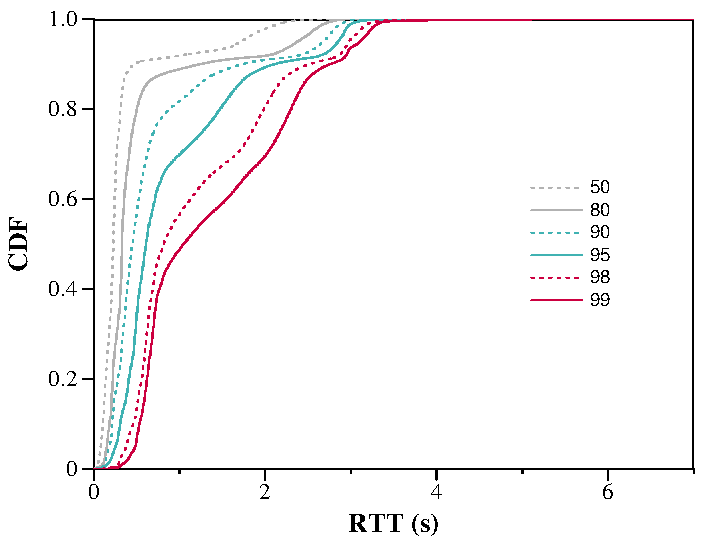
\includegraphics[width=0.7\textwidth]{timeouts/figs/cdf_raw_ping_ttl}
\end{center}
\caption{\label{fig:raw_lat}%
CDF of percentile latency of survey-detected responses per IP address: Each point represents an IP address
and each curve represents the percentile from that IP address's
response latencies. The slope of the latency
percentiles increases around the 3 second mark, suggesting that
ISI's prober timed out responses that arrived after 3 seconds.
}
\end{figure}

In this section, we present the latencies we would observe
when considering only those responses that were matched to 
requests because they arrived within the timeout.  We call 
these responses \emph{survey-detected responses}.

We aggregate round trip time measurements in terms of the
distribution of latency values per IP address, focusing on
characteristic values on the median, 80th, 90th, 95th, 98th
and 99th percentile latencies.  That is, we attempt to treat
each IP address equally, rather than treat each ping
measurement equally.  This aggregation ensures that
well-connected hosts that reply reliably are not
over-represented relative to hosts that reply infrequently.

Taking ISI survey datasets from 2011--2013 together, we show a CDF of
these percentile values considering only survey-detected
responses in Figure~\ref{fig:raw_lat}.  Taken literally, 95\%
of echo replies from 95\% of addresses will arrive in less than
2.85 seconds.  However, it is apparent that the distribution
is clipped at the 3 second mark, although a few responses
were matched even after 7 seconds.   

We observe three broad phases in this graph: (1) the lower
40\% of addresses show a reasonably tight distribution in
which the 99th percentile stays close to the 98th; (2) the
next 50\% in which the median remains low but the higher
percentiles increase; and (3) the top 10\% where the median
rises above 0.5 seconds.


\subsection{Unmatched responses}

If a probe takes more than three seconds to solicit a
response, it appears as if the probe timed-out and the
response was unsolicited or \emph{unmatched}.  Since it
appears from Figure~\ref{fig:raw_lat} that three seconds is
short enough that it is altering the distribution of round
trip times, we are interested in matching these echo
responses to construct the complete distribution of round
trip times.

Matching these responses to find \emph{delayed responses} is
not a simple matter, however.  In particular, we find two
causes of \emph{unexpected responses} that should not yield
samples of round trip times: unmatched responses solicited
by echo requests sent to broadcast addresses and apparent
denial of service responses.

% We require the union of low-rtt responses' latencies and high-rtt
% responses' latencies to perform an analysis of ping
% latencies. 
% \subsection{Matching delayed responses}

We match a delayed response with its corresponding request
as follows: Given an unmatched response having a source IP
address, we look for the last request sent to that IP
address.  If the last request timed out and has not been matched, the latency is then the difference between the
timestamp of the response and the timestamp of the
request.  ISI recorded the timestamp of unmatched responses
to a 1 second precision, thus the latencies of inferred
delayed responses are precise only to a second.

The presence of unexpected responses can lead to the
inference of incorrect latencies for delayed responses using
this technique: not all unexpected responses should be
matched by source address.
We thus develop filters to remove unexpected responses from the set of
unmatched responses.

We note that it is possible to match responses to requests
explicitly using the id and sequence numbers associated with
ICMP echo requests, and even perhaps using the payload.
These attributes were not recorded in the ISI dataset, which
motivates us to develop the source address based scheme.  We
use these fields when running Zmap or other tools to confirm
high latencies in Section~\ref{sec:verification} below.


% Some of
% these unmatched responses are higher latency responses which arrived
% at the prober after the timeout duration; we call these responses high-rtt
% responses. The remaining unmatched responses are unexpected responses, sent either
% in response to an echo request addressed to a broadcast address or as part
% of a Denial of Service attack. 

% \subsection{Unexpected Responses}
% 
% The dataset contains two sources of unexpected responses: Responses
% obtained from probes sent to broadcast addresses and
% duplicate responses.  We discuss each in turn. 
% Our goal is to study the latency of pings, including both low-rtt as
% well as high-rtt responses. To recover high-rtt responses from the
% data, we need to match unmatched echo Responses with their corresponding echo Requests.

% Have a figure here which shows the distribution of latencies from the
% raw pings, and how we found out that it has a 3 second timeout.
% ISI has a timeout of 3 seconds. Drop everything that arrives after
% then.

% When we tried reconstructing, we had to clean up a bunch. Had the
% following problems:

\subsubsection{Broadcast responses}

% We show that several unmatched responses are caused by
The dataset contains several instances where a ping to a
destination times out, but is closely followed by an
unmatched response from a source address that is within the same /24
address block, but different from the destination.
% The dataset contains several unmatched
% responses that were received immediately after a ping was sent to a different
% address within the same /24 address block.
In each round of probing, this behavior repeats.
%
Here, we analyze these unmatched responses, find that they are likely
caused by probing broadcast addresses, and filter them.

Network prefixes often include a broadcast address, where one
address within a subnet represents all devices connected to
that prefix~\cite{rfc919}.
%
The broadcast address in a network should
be an address that is
unlikely to be assigned to a real host~\cite{rfc919}, such as the
address whose host-part bits are all 1s or 0s, allowing us to
characterize broadcast addresses.
%
Devices that receive an echo
request sent to the broadcast address may, depending on
configuration, send a response~\cite{rfc1122}, and if sending a response,
will use a source address that is their own.
%
We call these
responses \emph{broadcast responses}.  
%
No device should send
an echo response with the source address that is the
broadcast destination of the echo request. 

% We investigate Echo Requests to destination addresses that trigger
% Echo Response from different addresses within the same /24 address blocks.
% We seek to understand why an Echo Request sent to a destination
% address would trigger an Echo Response from a different address within
% the same /24 address block.
% We hypothesize that a ping sent to broadcast address triggers
% responses from address(es) within the same /24 address block.
We hypothesize that pings that trigger responses from different
addresses within the same /24 address block result when the
ping destination is a broadcast address. 
We examine ping destinations
that solicit a response from a different address in the same /24
address block, and check if they appear to be broadcast addresses.
%
%
% These addresses will have last octets that
% can be represented as $2^n-1$ such as 63, 127, 255 etc.
%
% We wondered if network operators are following this convention.
%

We extended the ICMP probing module in the
Zmap scanner~\cite{durumeric2013zmap} to embed the destination
into the echo request, then to extract the destination from the
echo response.
%
Doing so allows us to infer the destination address to which the probe
was originally sent.
%
% We mark such a response as a
% broadcast response.
%
Zmap collected the data and made
it available for download at \url{scans.io}.
%

We choose the Zmap scan conducted closest in
time to the last ISI survey we studied, on April 17 2015, to investigate
the host-part bits of destination addresses that triggered responses
from a different address from the same /24 address block.
%
We plot the distribution of the last octets of these addresses in
Figure~\ref{fig:zmap_last_octet_hist}.
%
Last octets with the last N bits ending in 1 or 0, where N is greater than 1,
such as 255, 0, 127, 128 etc., have spikes. These addresses are likely broadcast addresses.
% Last octets with the last N bits as 1 (where N $>$ 1), such as 255, 127, etc., have the largest
% spikes. Last octets with the last N bits as 0, such as 0, 128, etc.,
% also have spikes, but smaller.
On the other hand, last octets that
end in binary '01' or '10' have very few addresses.

\begin{figure}[t]
\begin{center}
\includegraphics[width=3in]{timeouts/figs/zmap_last_octet_hist_all_bcast_addrs_apr_17}
\end{center}
\caption{\label{fig:zmap_last_octet_hist}%
Broadcast addresses that solicit responses in Zmap: Broadcast addresses usually
have last octets whose last N bits are either 1 or 0
(where N $>$ 1).
}
\end{figure}


\subsubsection*{Broadcast responses exist in the dataset}

% Next, we show the existence of broadcast responses in the ISI dataset.
% We examine how many of the unmatched responses in the dataset are
% broadcast responses. 
%
\begin{figure}[t]
\begin{center}
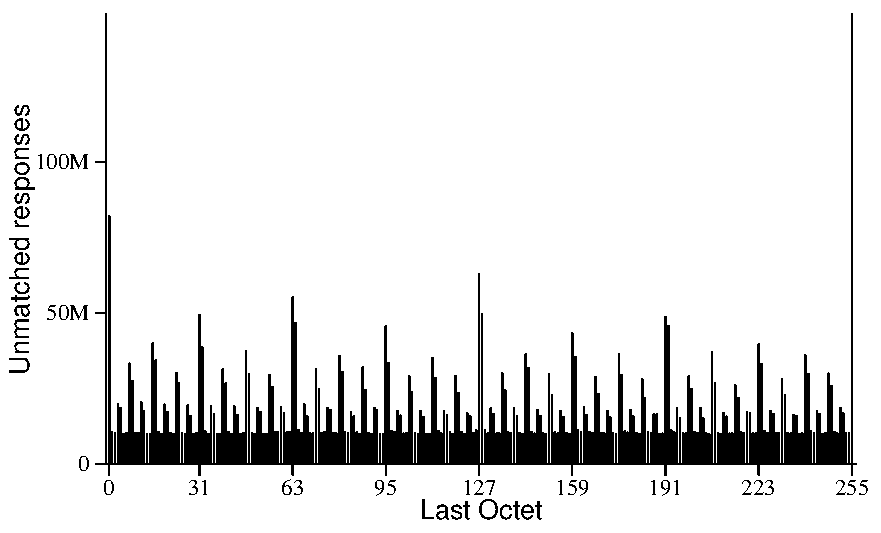
\includegraphics[width=.99\linewidth]{timeouts/figs/last_octet_hist}
\end{center}
\caption{\label{fig:bcast_hist}%
Number of unmatched responses that followed a probe sent to address
with last octet X. Last octets with last N bits ending in
0s and 1s (where N $>$ 1) observe spikes, likely caused by broadcast
responses. Not all unmatched responses are caused by broadcast
responses, however, since there exist roughly 10M unmatched
responses distributed evenly across all last octets.}
\end{figure}



We examine if unmatched responses in the ISI dataset are caused by pings sent to broadcast addresses.
%
Since broadcast responses are likely to be seen after an
Echo Request sent to a broadcast address, we find
the most recently probed address within the same /24 prefix for each
unmatched response. 
%
We then extract the last octet of the most recently probed
address.
%
Figure~\ref{fig:bcast_hist} shows the
distribution of unmatched responses across these last octets. 
%
We find that around 10M unmatched responses are distributed evenly
across all last octets: these are unmatched responses that don't seem
to be broadcast responses.
%
However, last octets that have their last N bits as 1s and 0s
,when N is greater than 1, observe spikes similar to those in Figure~\ref{fig:zmap_last_octet_hist}.
% , supporting our hypothesis that these are
% responses to broadcast addresses.
%
% These are the addresses most likely to see an
% unmatched response after an echo request to them times
% out. 
%

If left in the data, broadcast responses could yield
substantial latency overestimates in the following, common,
scenario, which we illustrate in
Figure~\ref{fig:bcast_sample}.
%
Assume that the echo request
sent to an address 211.4.10.254 is lost and that the
device is configured to respond to broadcast pings.  
%
The
echo request sent to 211.4.10.254 could then be matched to
the response to the request sent to 211.4.10.255, the
broadcast address of the enclosing prefix.  
%
This would lead
to a latency based on the interval between probing
211.4.10.254 and 211.4.10.255, as shown in the figure.

\begin{figure}[t]
\begin{center}
% \centering
% 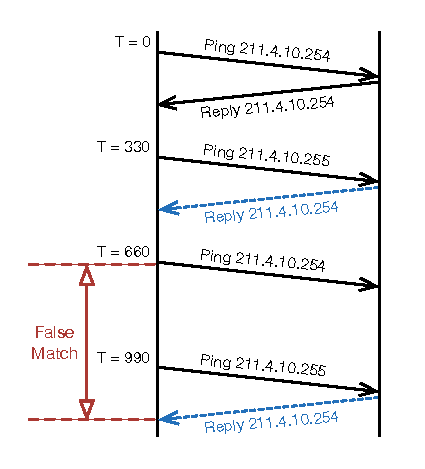
\includegraphics[width=0.97\linewidth]{timeouts/figs/wfall_bcast}
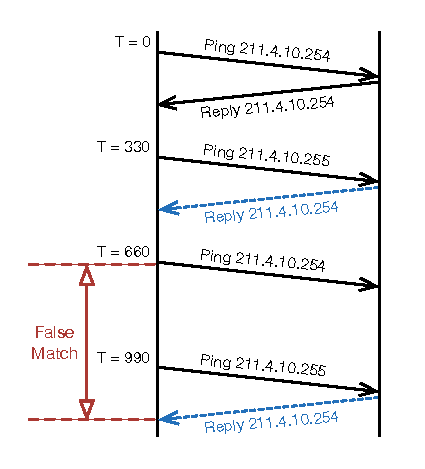
\includegraphics[width=3in]{timeouts/figs/wfall_bcast}
\end{center}
\caption{\label{fig:bcast_sample}%
We filter broadcast responses since they can lead to the inference of
false latencies. This figure illustrates a potential incorrect match
caused by a broadcast response.
Echo requests sent to the broadcast address 211.4.10.255 at T = 330
and T = 990 seconds solicit responses from 211.4.10.254.  When a timeout occurs 
for a request sent directly to 211.4.10.254 at T = 660 seconds, we 
would falsely connect that request to the response at T = 990 seconds.}
\end{figure}

%
% A last octet of 255 and 0 have particularly large spikes, 
% corresponding to the possible broadcast addresses of a /24 subnet.

\subsubsection*{Filtering broadcast responses}

% A potential approach to filtering broadcast responses is to check
% if an unmatched response was preceded by a ping to an address
% whose last octet had its last N bits as 1s or 0s (where N $>$ 1).
% %
% However, this scheme would have been too aggressive, potentially filtering
% delayed responses that coincidentally happened to arrive after an Echo
% Request to a broadcast address.
% %
% Thus, we develop an alternate method which uses ISI's non-random probing
% scheme to detect addresses that source broadcast responses.
%
We develop a method which uses ISI's non-random probing
scheme to detect addresses that source broadcast responses.
We call such addresses \emph{broadcast responders}, and seek to filter
all their responses.
 % and the assumption that broadcast responses, like typical Echo
% responses, have stable latencies.
%
We believe that delayed responses are likely to
exhibit high variance in their response latencies, since congestion varies over
time. 
%
On the other hand, a
broadcast response is likely to have relatively stable latency.
%
% (unless it happens to be congested too.)

ISI's probing scheme sends
probes to each address in a /24 address block in a nonrandom sequence,
allowing us to develop a filter that checks if a source address responds
to a broadcast address each round.
%
% The last octet of the probed IP address generally has its $n$th
% bit (counting from 0) swapped every $2^n$ probes on the /24 block.
Addresses are probed such that last octets that are off by one, such
as 254 and 255, receive pings spaced 330 seconds apart (half the
probing interval of 11 minutes) as shown in Figure~\ref{fig:bcast_sample}.
% nth most significant bit probed, i.e., probes to 1 and 129 are sent
% one after the other.
%
% We filter broadcast responses by looking for unmatched responses from
% the same source address that
% repeat periodically with similar latency.
%
For every unmatched response with a latency of at least 10 seconds,
the filter checks if the same source address had sent an unmatched
response with a similar latency in the previous round.
% checks whether they occurred right before another response of a
% similar latency (within 2 seconds).
%
We take an exponentially weighted moving average of the number of times
this occurs for a given source address with $\alpha=0.01$.
%
Most broadcast responders have the
maximum of this moving average $>$ 0.9, but since probe-loss can
potentially decrease this value, we mark IP addresses with values $>$
0.2 and filter all their responses. 
%
% If the maximum of this moving average per source address is greater than 0.2, the IP address
% is marked as one that responds to probes to broadcast addresses, and
% it is filtered out.
% %
% This filter is meant to be selective for the specific pattern of responses, without being so
% selective that it fails to classify broadcast addresses in the
% presence of loss.

We confirm that we find broadcast responders correctly in the
ISI surveys by comparing the ones we found in the ISI 2015 surveys
with broadcast responders from the Zmap dataset.
%
% Ideally, the Zmap scan should have been conducted at the same time as
% the ISI surveys, but we choose the closest available Zmap scan in time,
% bearing in mind that broadcast responders may change over time.
%
% The IT63w (20150117)
% and IT63c (20150206) datasets recorded responses from 4,008,830
% addresses.
% %
% The filter detected 9,942 broadcast responders among them.
%
% 8729 of these broadcast responders appeared as the source addresses
% of an Echo Response in Zmap's
% April 17 2015 scan. 
%
Zmap detected 939,559 broadcast responders in the April 17
2015 scan, of which 7212 had been
addresses that provided Echo Responses in ISI's IT63w (20150117) and
IT63c (20150206) datasets.
%
The filter detected 7044 (97.7\%) of these as broadcast responders. 
% We inspected the remaining 168 addresses and found that 159 could not have been broadcast responders at the time they were probed by ISI: their 99th percentile RTTs were far too low.
We inspected the 168 remaining addresses and found that 154 addresses
have 99th percentile latencies below 2.5 seconds. Since ISI
probes a /24 prefix only once every 2.5 seconds, these addresses
cannot be broadcast responders. Another 5 addresses have 99th
percentiles latencies below 5 seconds; these are unlikely to be
broadcast responders as well.

The remaining 9 addresses had 99th percentile latencies in excess of
300s and seem to be broadcast responders. Upon closer inspection, we
found that these addresses only occasionally sent an unmatched
response: around once every 50 rounds. The $\alpha$ parameter of the
filter can tolerate some rounds with missing responses, but these
addresses respond in so few rounds that they pass undetected. 
If these 9 are indeed broadcast responders as suggested by high 99th percentile latencies, this yields a false negative rate of our filter of 0.13\%.
% demonstrating that it is able to find broadcast responders with high
% accuracy.

\subsubsection{Duplicate responses}

Packets can be duplicated.  A duplicated packet will not affect inferred latencies as
long as the original response to the original probe packet reaches the prober, since our scheme
ignores subsequent duplicate responses. However, we find that some IP
addresses respond many times to a single probe. In this case, the incoming packets aren't responses to
probes, but are either caused by incorrect configurations or malicious
behavior. 

\begin{figure}[t]
\begin{center}
% \centering
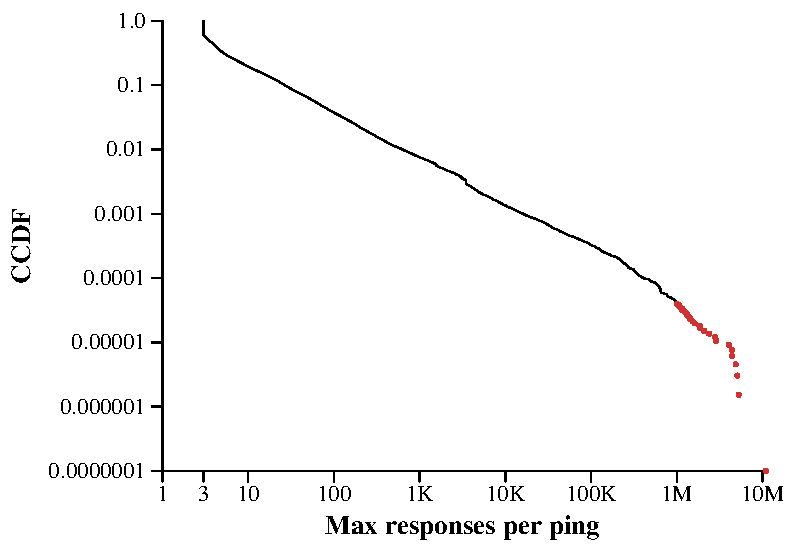
\includegraphics[width=.9\linewidth]{timeouts/figs/ccdf_dos}
\end{center}
\caption{\label{fig:dos}%
Maximum number of responses received for a single echo request, for IP
addresses that sent more than 2 responses to an echo request. The red
dots indicate instances where addresses responded to a single echo
request with more than 1M echo responses. We believe that these are
caused by DoS attacks.}
\end{figure}

Figure~\ref{fig:dos} shows the distribution of the maximum number of
echo responses observed in response to a single echo request. Since
broadcast responses can also be interpreted as duplicate responses, we
look only at IP addresses that sent more than 2 echo responses for an
echo request. Of 658,841 such addresses, we find that 4,985 (0.7\%) sent
at least 1,000 echo responses. The red dots in the figure show 26
addresses that sent more than one million echo
responses, with one address sending nearly 11 million responses in 11 minutes.

Zmap authors reported that they observed
retaliatory DoS attacks
in response to their Internet-wide probes~\cite{durumeric2013zmap}. We believe that
some of the responses in the ISI dataset are also caused by DoS attacks.

We filter duplicate responses by ignoring IP addresses that ever
responded more than 4 times to a single echo request, based on observing the
distribution of duplicates shown in Figure~\ref{fig:dos}.  Packets can
sometimes get duplicated on the Internet, and we want to be selective
in our filtering to remove as little as necessary.  Even if a response from
the probed IP address is duplicated and a broadcast response is also
duplicated, there should be only 4 echo responses in the dataset. We
believe that IP addresses observing more than 4 echo responses to a
single echo request are either misconfigured or are participating in a DoS attack.
In either case, the latencies are not trustworthy.


% \vfill\eject
\section{Recommended Timeout Values}
\label{sec:eval}
% \newcommand{\hdr}[1]{\multicolumn{1}{c}{\textbf{#1}}}

In this section, we analyze the ping latencies of all pings obtained
from ISI's Internet survey datasets from 2015 to find reasonable timeout values.
We demonstrate the effectiveness
of our matching scheme for recovering delayed responses from the
dataset. We then group the survey-detected responses and delayed
responses together to determine what timeout values would be necessary to 
recover various percentiles of responses. 
Some IP
addresses observe very high latencies in the ISI dataset; we verify that
these are real in Section~\ref{sec:verification} and examine causes in Section~\ref{sec:causes}.

% we validate
% our results by probing these IP addresses with the scamper tool~\cite{luckie2010scamper} and
% analyzing their latencies.

\subsection{Incorporating unmatched responses}

\begin{table}[tb]
  \begin{center}
    \begin{small}
  \begin{tabular}{c|rr}
    & \hdr{Packets} & \hdr{Addresses} \\
    \hline
    \textbf{Survey-detected } & 9,644,670,150 & 4,008,703\Tstrut\\
    % \hline
    \textbf{Naive matching} & 9,768,703,324 & 4,008,830 \\
    % \hline
    \textbf{Broadcast responses} & 33,775,148 & 9,942 \\
    % \hline
    \textbf{Duplicate responses} & 67,183,853 & 20,736 \\
    % \hline
    % \textbf{Filtered survey-detected} & 125,578,194,082 & 16,320,357 \\
    % \hline
    \textbf{Survey + Delayed} & 9,667,744,323 & 3,978,152 \\
    \end{tabular}
    \end{small}
  \end{center}
    \caption[Adding unmatched responses to survey-detected responses]{
\label{tbl:filter_results}
Adding unmatched responses to survey-detected responses}
\end{table}

\begin{figure*}[tb]
\begin{subfigure}[t]{0.47\linewidth}
\centering
\includegraphics[width=\linewidth]{timeouts/figs/cdf_basic_ping_ttl}
\caption{
\label{fig:basic_lat}
Before filtering
}
\end{subfigure}
%
\hfill
%
\begin{subfigure}[t]{0.47\linewidth}
\centering
\includegraphics[width=\linewidth]{timeouts/figs/cdf_filter_ping_ttl}
\caption{
\label{fig:filter_lat}
After filtering
}
\end{subfigure}
\caption{
\label{fig:lat} 
CDF of Percentile latency per IP address before and after filtering
  unexpected responses. Each point represents an IP address and each
  color represents the percentile from that IP address's response
  latencies. Before filtering unexpected responses, there are
  bumps caused by broadcast responses at 330s, 165s and 495s,
  fractions of the 11 minute (660s) probing interval.
}
\end{figure*}


ISI detected 9.64 Billion echo responses from 4 Million IP addresses in 2015
in the IT63w (20150117) and IT63c (20150206) datasets, as shown in the
first row of Table~\ref{tbl:filter_results}.
The next row shows the number of responses we would have obtained
if we had used a naive matching scheme where we simply matched each
unmatched response for an IP address with the last echo request for
that IP
address, without filtering unexpected responses.
The number of responses
increases by 1.3\% to 9.77 Billion; however, this includes responses
from addresses that received broadcast responses and duplicate
responses. 
%
After filtering unexpected responses, the number of IP addresses
reduces to 99.23\% of
the original addresses. 
%
Of 30,678 discarded IP addresses, 9,942 (32.4\%)
addresses were discarded because they also received broadcast
responses. 
%
The majority of discarded IP addresses, 20,736 (67.6\%) were addresses that
sent more than 4 echo responses in response to a single echo request. 

Though the number of discarded IP addresses is relatively small, removing
them eliminates responses that cluster around 330, 165, and 495 seconds.
Figure~\ref{fig:lat} shows the distribution of percentile latency per
IP address before and after filtering unexpected responses.  Comparing
these two graphs shows that the ``bumps'' in the CDF are removed by the filtering.

After discarding addresses, our matching technique yields 23,074,173
additional responses for the remaining addresses, giving us a total of
9.67 Billion Echo Responses from 3.98 Million IP addresses. We perform
our latency analysis on this combined dataset.

% They are caused
% because of the non-random sequence of probing, which meant that 0 and
% 1 were probed 330seconds apart.

% \newcommand{\bb}{~~~~~}
%%% \begin{table}[tp]%
%%%   \begin{center}%
%%%   \begin{small}%
%%%   \begin{tabular}{c@{\hspace{0.5em}}r|rrrrrrr}
%%%     &\multicolumn{8}{c}{\textbf{\% of pings}\vspace{0.3em}} \\
%%%     && \hdr{1\%} & \multicolumn{1}{c}{\textbf{50\%}} & \hdr{80\%} & \hdr{90\%} & \hdr{95\%} &
%%%     \hdr{98\%} & \hdr{99\%} \\\cline{2-9}
%%%     \parbox[t]{2mm}{\multirow{7}{*}{\rotatebox[origin=c]{90}{\textbf{\% of addresses}}}} & 
%%%     \textbf{1\%} & 0.01 & 0.05 & 0.11 & 0.13 & 0.16 & 0.29 & 0.34 \\
%%% %    \cline{2-9}
%%%     &\textbf{50\%} & 0.12 & 0.24 & 0.35 & 0.50 & 0.67 & 0.92 & 1.21 \\
%%% %    \cline{2-9}
%%%     &\textbf{80\%} & 0.19 & 0.33 & 0.57 & 1.34 & 2.20 & 5\bb & 7\bb \\
%%% %    \cline{2-9}
%%%     &\textbf{90\%} & 0.24 & 1.00 & 2.39 & 4\bb & 6\bb & 8\bb & 11\bb \\
%%% %    \cline{2-9}
%%%     &\textbf{95\%} & 0.31 & 2.43 & 5\bb & 6\bb & 7\bb & 12\bb & 18\bb \\
%%% %    \cline{2-9}
%%%     &\textbf{98\%} & 0.37 & 4\bb & 6\bb & 7\bb & 11\bb & 20\bb & 52\bb \\
%%% %    \cline{2-9}
%%%     &\textbf{99\%} & 0.43 & 4\bb & 6\bb & 8\bb & 14\bb & 55\bb & 159\bb \\
%%%     \end{tabular}
%%%   \end{small}
%%%   \end{center}
%%% 
%%% 
%%%     \caption{Minimum timeout in seconds that would have captured c\% of pings from r\% of IP
%%%       addresses in pings sent from Nov 2011 to October 2013 (where r is the row number and c is
%%%       the column number).}
%%% \label{tbl:grand}
%%% \end{table}

%\newcommand{\bb}{~~~~~}


\subsection{Recommended Timeout Values}

We now find retransmission thresholds which recover various
percentiles of responses for the IP addresses from the
combined dataset. For each IP address, we find the 1st, 50th, 80th,
90th, 95th, 98th and 99th percentile latencies. We then find the 1st, 50th,
80th, 90th, 95th, 98th and 99th percentiles of all the 1st percentile latencies. We repeat this for each
percentile and show the results in Table~\ref{tbl:grand_2015}.

\begin{table}[tb]
  % \begin{center}%
    \begin{small}%
      \hspace{-0.06in}%
  \begin{tabular}{l@{\hspace{0.5em}}r|rrrrrrr}
    &\multicolumn{8}{c}{\textbf{\% of pings}} \\
    && \hdr{1\%} & \multicolumn{1}{c}{\textbf{50\%}} & \hdr{80\%} & \hdr{90\%} & \hdr{95\%} &
    \hdr{98\%} & \hdr{99\%} \\\cline{2-9}
    \multirow{7}{*}{\rotatebox[origin=lb]{90}{\textbf{\% of addresses}}} & 
    \textbf{1\%} & 0.01 & 0.03 & 0.04 & 0.07 & 0.10 & 0.13 & 0.18\Tstrut \\
%    \cline{2-9}
    &\textbf{50\%} & 0.16 & 0.19 & 0.21 & 0.26 & 0.42 & 0.53 & 0.64 \\
%    \cline{2-9}
    &\textbf{80\%} & 0.19 & 0.26 & 0.33 & 0.43 & 0.54 & 0.74 & 1.21 \\
%    \cline{2-9}
    &\textbf{90\%} & 0.22 & 0.31 & 0.42 & 0.57 & 0.84 & 1.61 & 3\bb \\
%    \cline{2-9}
    &\textbf{95\%} & 0.25 & 1.42 & 2.38 & 3\bb & 5\bb & 9\bb & 15\bb \\
%    \cline{2-9}
    &\textbf{98\%} & 0.30 & 1.94 & 4\bb & 6\bb & 12\bb & 41\bb & 78\bb \\
%    \cline{2-9}
    &\textbf{99\%} & 0.33 & 2.31 & 4\bb & 8\bb & 22\bb & 76\bb & 145\bb \\
    \end{tabular}
    \end{small}
    % \end{center}

\vspace{\baselineskip}
    \caption[Minimum timeouts]{Minimum timeout in seconds that would have captured c\% of pings from r\% of IP
      addresses in the IT63w (20150117) and IT63c (20150206) datasets (where r is the row number and c is
      the column number).}
\label{tbl:grand_2015}
\end{table}

The 1st percentile of an address's latency will be close to the ideal latency that its link
can provide. We find that the 1st percentile latency is below 330ms for 99\%
of IP addresses: most addresses are capable of
responding with low latency. Further, 50\% of pings from 50\% of the
addresses have latencies below 190ms, showing that latencies tend to
be low in general.

However, we see that a substantial fraction of IP addresses also have
surprisingly high latencies. For instance, to capture 95\% of pings from 95\%
addresses requires waiting 5 seconds.  Restated, at least 5\% of
pings from 5\% of addresses have latencies higher than 5 seconds. Thus, even
setting a timeout as high as 5 seconds will infer a false loss rate of 5\%
for these addresses.

Note that retrying lost pings cannot be used as a substitute for
setting a longer timeout since a retried ping is not an independent
sample of latency. 
Whatever caused the first one to be delayed is likely to cause the
followup pings to be delayed as well, as we show in Section~\ref{sec:causes}.

At the extreme, we see 1\% of pings from 1\% of addresses
having latency above 145 seconds! These latencies are so high that
we investigate these addresses further.  \emph{We now
  consider 60 seconds to be a reasonable timeout to balance
  progress with response rate, at least when studying
  outages and latencies, although an ideal timeout may vary
  for different settings.}  A timeout of 60 seconds easily
covers 98\% of pings to 98\% of addresses, yet does not seem
long enough to slow measurements unnecessarily.


\section{Verification of long ping times}
\label{sec:verification}

In this section, we address doubts that long observed ping
times are real: that they are a product of ISI's probing scheme, that
they might be caused by errors in a particular data set, or that they might derive from
discrimination against ICMP.

\subsection{Are high latencies observed by other probing schemes?}

Some of the latencies in Table~\ref{tbl:grand_2015} are so high that
we considered if they could be artifacts of ISI's probing scheme. We
investigate latencies obtained using two other probing techniques,
Zmap and scamper, and check if the high latencies observed in the ISI datasets are reproducible.
%  We confirm that each observes the
% occurrence of long ping times.
% We use the scamper tool to probe a subset of high
% latency addresses and 



\subsubsection*{Does Zmap observe high latencies?}
% \paragraph{Zmap observes high latencies}

We check for high latencies using the Zmap scanner~\cite{durumeric2013zmap}. 
%
As part of our extension of the ICMP probing module in the
Zmap scanner, we also embed the probe send time into the echo request,
and extract it from the
echo response, allowing us to estimate the RTT, albeit without the
precision of kernel send timestamps.
%
% Zmap collected the data and made
% it available for download at \url{scans.io}.

Zmap has performed these scans since April 2015. Scans have been conducted over a range of different times,
different days of the week and across four months in 2015 (as of Sep
5, 2015), as shown in Table~\ref{tbl:scans}. Typically, scans were performed on Sundays or Thursdays, beginning
at noon UTC time. However, the scans on April 17, May 22, and June 15
were conducted on other days and at other times, increasing diversity. Each Zmap scan
takes 10 and a half hours to complete and recovers Echo Responses from
around 350M addresses.
%

\begin{table}[tb]
  \begin{center}
    \begin{tiny}
  \begin{tabular}{r|c|c|c}
    \hdr{Scan Date} & \hdr{Day} & \hdr{Begin Time} & \hdr{Echo Responses} \\
    \hline
    \textbf{Apr 17, 2015} & Fri & 02:44 & 339M\Tstrut \\
    \textbf{Apr 19, 2015} & Sun & 12:07 & 340M \\
    \textbf{Apr 23, 2015} & Thu & 12:07 & 343M \\
    \textbf{Apr 26, 2015} & Sun & 12:07 & 343M \\
    \textbf{Apr 30, 2015} & Thu & 12:08 &  344M \\
    \textbf{May 3, 2015} & Sun & 12:08 & 344M \\
    \textbf{May 17, 2015} & Sun & 12:09 &  347M \\
    \textbf{May 22, 2015} & Fri & 00:57 & 371M \\
    \textbf{May 24, 2015} & Sun & 12:09 &  369M \\
    \textbf{May 31, 2015} & Sun & 12:09 & 362M \\
    \textbf{Jun 4, 2015} & Thu & 12:10 & 368M \\
    \textbf{Jun 15, 2015} & Mon & 13:53 & 357M \\
    % \hline
    \textbf{Jun 21, 2015} & Sun & 12:11 & 368M \\
    % \hline
    \textbf{Jul 2, 2015} & Thu & 12:00 & 369M \\
    \textbf{Jul 5, 2015} & Sun & 12:00 & 368M \\
    \textbf{Jul 9, 2015} & Thu & 12:00 & 369M \\
    \textbf{Jul 12, 2015} & Sun & 12:00 & 367M \\
    \end{tabular}
    \end{tiny}
  \end{center}
    \caption[Details of Zmap scans used in the analyses]{Zmap scan details: For each Zmap scan in
      Figure~\ref{fig:grand_zmap}, the table shows the date, day of the
      week, the time at which the scan began (in UTC time), and the number of
      destinations that responded with Echo Responses.}

\label{tbl:scans}
\end{table}

We choose all
available scans and 
analyze the distribution of
RTTs for the Echo Responses in
Figure~\ref{fig:grand_zmap}. 
%
Most responses arrive with low latency, having a median latency lower than
250ms for each scan.
%
However, ~5\% of addresses responded with RTTs greater than 1 second
in each scan. Further, 0.1\% of addresses responded with latencies exceeding
75 seconds in each scan although the 99.9th percentile
latency exhibited some variation: the May 22 scan had the lowest 99.9th percentile
latency (77 seconds) whereas the July 9 scan had the highest (102 seconds).
%
We infer from these nearly identical latency distributions that high latencies are persistent for a consistent fraction of addresses.
% To compare the distribution of RTTs requires choosing a
% comparable sample from the survey data, given that it
% reprobes addresses for weeks.  We used the latency of the
% first received ping from each address in the IT63c
% (20150206) and IT63w (20150117) datasets.  

% Figure~\ref{fig:zmap_vs_isi_2015} shows the distribution of RTTs. 5\%
% of addresses have latencies $>$ 1s in each.

% \begin{figure}[tbh]
% \centering
% \includegraphics[width=3in]{figs/zmap_vs_isi_2015}
% \caption{\label{fig:zmap_vs_isi_2015}%
% Distribution of RTTs for three Zmap scans and
% two ISI surveys performed in 2015. 5\% of addresses have latencies $>$
% 1s in each.
% }
% \end{figure}

\begin{figure}[tb]
% \centering
\begin{center}
\includegraphics[width=3in]{timeouts/figs/grand_zmap}
\end{center}
\caption[Distribution of RTTs for all Zmap scans performed in 2015]{\label{fig:grand_zmap}%
Distribution of RTTs for all Zmap scans performed in 2015. Around 5\%
of addresses have latencies greater than 1s in each scan, and 0.1\% of addresses observed latencies in excess of 75s.
}
\end{figure}

% \vspace{-0.1in}

\subsubsection*{Does scamper also observe high latencies?}
% \paragraph{Scamper also observes high latencies}
Both ISI and Zmap probe millions of addresses, and we investigate
whether latencies are affected by these probing schemes
triggering rate-limits or firewalls. We select a small sample of
addresses that are likely to have high latencies from the
ISI dataset, probe them using scamper~\cite{luckie2010scamper}, and check for unusually high latencies.

In the 2011 - 2013
ISI dataset, 20,095 IP
addresses had at least 5\% of their pings with latencies 100 seconds and above. We chose 2000 random IP addresses from
this subset and sent 1000 pings to them, once every 10 seconds using
scamper~\cite{luckie2010scamper} and analyzed the responses. 
In this
analysis, we used scamper's default packet response matching
mechanism: so long as scamper continues to run, received responses
will be matched with sent packets. Because we used scamper's defaults,
scamper ceased to run 2 seconds after the last packet was sent, so
we missed responses to the last few pings that arrived after
scamper ceased running. Although scamper can
be configured to wait longer for responses, in later analyses, we ran tcpdump simultaneously and matched
responses to sent packets separately.

Of the 2000 addresses, 1244 responded to our probes.
Figure~\ref{fig:cdf_high_rtt_ips} shows the percentile latency per IP
address. The 95th percentile latency for 50\% of the addresses is now
considerably lower, at 7.3s. This suggests that addresses prone to extremely high
latencies vary with time: we investigate addresses with
this behavior further in Section~\ref{sec:causes}. 

Nevertheless, Figure~\ref{fig:cdf_high_rtt_ips} shows that scamper
also observes some instances of very high latencies. 17\%
of addresses observe latencies greater than 100 seconds for 1\%
of their pings. We therefore rule out the possibility that the high
latencies are a product of the probing scheme.

% , and show that they addresses tend
% to be from cellular Autonomous Systems which exhib


\begin{figure}[tb]
\begin{center}
% \centering
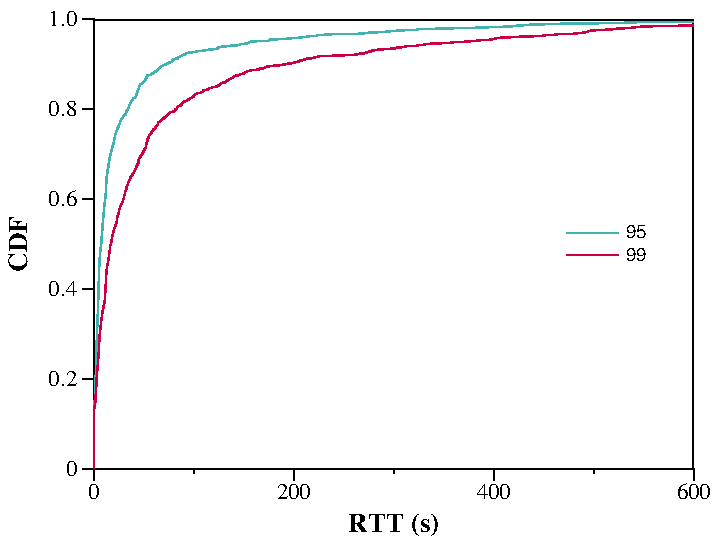
\includegraphics[width=3in]{timeouts/figs/cdf_high_rtt_guys_grand}
\end{center}
\caption[Confirmation of high latency with Scamper]{\label{fig:cdf_high_rtt_ips}%
Confirmation of high latency: Percentile latency per IP address for
2000 randomly chosen IP addresses from ISI's 2011 - 2013 surveys that had $>$ 5\% of pings with
latencies 100s and above. Each point represents an IP address and the
lines represent the percentile latency from that IP address. 17\% of
them continue to observe 1\% of their pings with
latencies $>$ 100s.
}
\end{figure}

% \subsection{Are ISI's sampled addresses representative?}

% ISI's methodology involves probing a sample of the address
% space.  It would be reasonable to expect that perhaps this
% sampling affects observed latencies.  An underestimate might
% occur because a fraction of the ISI survey prefixes have
% been repeated since 2006, so such addresses may be in a more
% established part of the network.  On the other hand,
% latencies might be overestimated by bad luck, repeatedly probing a
% particularly slow prefix. 


% 0.1% of pings arrived after: April : 90, May : 77,  June : 83, Julys
% : 102

% per dataset analysis (time)
\ninput{timeouts/per_dataset}

\ninput{timeouts/is_it_icmp}

\subsection{Summary}

In this section, we confirmed that extremely high latencies are also observed by
techniques besides ISI's. We find that the high latencies are
not a result of a few individual ISI datasets, even though some
did appear atypical.  Further, high latencies affect all
protocols the same. 

We also found that the prevalence of high latencies has been increasing
since 2011. In 2015, a consistent 5\% of addresses have
latencies greater than a second. 

%% 
%% * could it be routing? (if affecting all of a /24 at the same time;  I don't believe this happens)
%% 
%% * could it be handoff?  (should be occasional / rare (though not necessarily so), within some networks but not all, and apply to networks with already high latencies)
%% 
%% * could it be solar interference on satellites?  (seek diurnal patterns s.t. for one (15 minute?) period out of the 24 hours, there's a problem)
%% 
%% * does it affect thought-to-be-wired links?  (seek large cable-provider networks and fiber providers, determine whether there are high latency guys in there.)
%% 
%% * can the devices be fingerprinted? (e.g., nmap)

\section{Why do pings take so long?}
\label{sec:causes}

In this section, we aim to determine what causes high RTTs. We
investigate the RTTs of satellite
links and find that they account for a small fraction of high RTT
addresses. We follow up with an analysis of Autonomous Systems and
geographic locations that are most prone to two potentially different
types of high RTTs: RTTs greater than 1s and RTTs greater than
100s. We then investigate addresses that exhibit each type of RTT and
find potential explanations.
% check if the first ping to an address in a continuous stream of pings is subject to
% higher latencies than the rest. Finally, we investigate particularly high
% latencies and identify patterns associated with their occurrence.

\ninput{timeouts/satellites}

\ninput{timeouts/zmap_asn_analysis}

\ninput{timeouts/first_ping}

\ninput{timeouts/handoff}

\subsection{Summary}
High latencies appear to be a property mainly of cellular
  Autonomous Systems, though a few also appear on satellite
  links. Latencies in the ISI data that are regularly above one second seem to be caused
by the first-ping behavior associated with several addresses, where
the first ping in a stream of pings has higher latency than the
rest. Egregiously high latencies, i.e., latencies greater than a
hundred seconds, occur in two broad patterns. In the first, latencies
steadily decay with each probe, as if clearing a backlog. In the second, latencies are continuously
high and are accompanied by loss, as if the network link is oversubscribed.



\section{Conclusion and Discussion}

Researchers use tools like ping to detect network outages,
but generally guessed at the timeout after which a ping
should be declared ``failed'' and an outage suspected.  The
choice of timeout can affect the accuracy and timeliness of
outage detection: if too small, the outage detector may
falsely assert an outage in the presence of congestion; if
too large, the outage detector may not pass the outage along
quickly for confirmation or diagnosis.

We investigated the latencies of responses in the ISI survey
dataset to determine a good timeout, considering the
distributions of latencies on a per-destination basis.
Foremost, latencies are higher than we expected, based on
conventional wisdom, and appear to have been increasing.
We show that these high latencies are not an artifact of
measurement choices such as using ICMP or the particular
vantage points or probing schemes used, although different data sets vary somewhat.
We show that high latencies are not caused by links with a substantial
base timeout, such as satellite links.  
% 
% 
% We analyzed the latencies of echo responses, including
% unmatched responses in the ISI survey data set, to determine
% what timeout would capture different fractions of
% responses from different fractions of remote IP addresses.
% We showed that high latencies are not an artifact of ISI
% data. % , and in fact, it may underestimate the extent of large latencies by sampling.
% We showed that high latencies are not an artifact of using ICMP
% echo requests: prioritization that might favor data-carrying TCP or UDP
% protocols does not have this substantial of an effect.
% We showed that high latencies have been increasing over the
% last few years by comparing different surveys taken at different times.
% We showed that satellite links are not particularly blameworthy
% in requiring high timeout values.
Finally, we showed that in many instances, the initial communication to
cellular wireless devices is largely to blame for high latency measures.
Similar spikes that may be consistent with handoff also dissipate over time,
to more conventional latencies that support application traffic.
With this data, researchers should be able to reason about
what to expect in terms of false outage detection for a
given timeout and how to design probing methods to account for
these behaviors.

% Our initial hypothesis was that it would be a simple matter
% to confirm that widely used timeout values would be adequate
% for studying outages, or failing that, that one or two
% additional seconds would be enough.
As memory capacity and performance becomes less of a
limiting factor, we believe that the lesson of this work is
to design network measurement software to approach outage
detection using a method comparable to that of TCP: send
another probe after 3 seconds, but continue listening for a
response to earlier probes, at least for a duration based, at
least in part, on the error rates implied by
Table~\ref{tbl:grand_2015}. 
% We plan
% to use 60 seconds when we need a timeout, and avoid timeouts
% otherwise.

% a per-ISP
% and per-region basis, since there can be wide variation in
% latencies. This work provides timeout values that would capture most
% pings (say 99\%) per-ISP and per-region. 

% The wide variation in observed latencies for IP addresses around the
% world indicate that probers should set timeout values
% based upon the addresses that they are probing. Even a 3s
% timeout may suffice for 90\% of addresses in the ISI survey since 90\% of addresses respond
% within 3s for 99\% of the pings sent to them. 

If investigating historical outage measurement data collected by
probing based techniques, the timeouts used by the technique must be
compared with timeouts that would have captured almost all responses
for the addresses pinged by the technique. For example, Thunderping
probes addresses only in the U.S. For these addresses, both the ISI
and Zmap datasets showed that more than 99\% of ping responses arrived
within the 5s timeout used by Thunderping. The probability of false
outage inferences due to high latency is small. However, if the Thunderping
technique had been used to ping addresses in South American cellular
ISPs, there would be a significantly higher probability of detecting
false outages, since the 5s timeout would have missed many delayed responses.

% In cases where a timeout is 


% My proposed work is to find expected latency values
% associated with the IP addresses that need to be probed, and to set
% their timeouts accordingly.
 
% I propose to find expected latencies for any IP address on the
% Internet by analyzing historical and current ping data, available from
% the Zmap project~\cite{censys-icmp}. Zmap has continued to perform
% their scans of the IPv4 Internet, averaging one scan per week since
% April 2015. For each IP address that has consistently responded to
% pings, I expect to have roughly 100 samples. I will calculate expected
% latencies for all addresses using their own latencies weighted by the
% number of observed samples and will also include latency samples of
% other ``related'' addresses. Related addresses can be addresses
% belonging to the same /24 network, addresses belonging to the same
% ISP, addresses sharing the same last-hop router, addresses from the
% same dynamically addressed pools etc; I describe related addresses in
% more detail in Section~\ref{sec:last_mile}.

% Once I have determined the expected latencies for all IP addresses
% that respond to pings in the IPv4 Internet, the next task is to
% determine appropriate per-address timeouts based upon the destinations
% that need to be probed. Given any address to probe, I will modify the probing scheme to
% set timeouts that are just high enough as to capture almost all
% responses (say 99.9\%) from that address. Setting adaptive timeouts this way will achieve the
% twin goals of capturing most responses while also keeping the state
% required at the prober low.


\chapter{Mitigating false inferences due to dynamic addressing}

\label{cpt:addr_change}

% TODO: Index section numbers to the roadmap

In this chapter, I begin by describing a common assumption---that IP
addresses can be used as proxies---for users in
Section~\ref{sec:addrs-are-host-proxies}. In
Section~\ref{sec:addrchange-false-inferences}, I discuss how dynamic
addressing can lead probing-based outage detection techniques to make
false inferences about outages.

Next, I describe work with colleagues to empirically
measure the frequency of dynamic addressing and the durations for
which addresses are assigned to residential home router devices in
several networks around the world and the effect of outages upon
dynamic reassignment~\cite{addrchange-reasons}. The measurements we
used are sourced from the RIPE NCC's Atlas project, which deploys small devices, called probes, that
conduct measurements from globally distributed
networks~\cite{atlas}. The RIPE Atlas dataset offers measurements that allow us to
determine when an IP address change occurred and what the addresses
were before and after the change. In addition, the dataset includes many
measurements that provide context about what was happening around the
time of the address change. I was able to use these measurements to
detect when RIPE Atlas probes rebooted and were not sending pings
(indicating a power outage) and when their pings were not getting
responses (indicating a network outage). In a study with colleagues of active RIPE
Atlas probes in 2015, we found 3,038 RIPE Atlas probes with address
changes hosted across 929 ISPs and 156
countries~\cite{addrchange-reasons}. Using the measurements from RIPE Atlas, I identify networks
where addresses are typically stable. 

Finally, in section~\ref{sec:complementary-ns} I discuss a technique to identify outages even in networks
where dynamic reassignment is common. Using a complementary dataset
that allows checking if an address for which a probing-based technique
detected an outage has remained the same before and after the detected
outage, we are able to confirm outages even in networks where dynamic
reassignment is common.

\section{IP addresses can be proxies for end users}

\label{sec:addrs-are-host-proxies}

Academia and industry often rely on a simplifying assumption that IP
addresses uniquely identify
end-hosts~\cite{p2pfilesharing,p2pavail,sen2004analyzing,sekar2006multi,anomalousdns,kuhrer2015going,xie2005worm,jung2004empirical,fabian2007botnet,stone2009your,andriesse2015reliable,fail2ban,spamhaus,cbl,sorbs}. This
assumption allows researchers to track end host behavior over
time~\cite{anomalousdns, kuhrer2015going, pingin}, or to count
participating users in peer-to-peer
systems~\cite{p2pfilesharing,p2pavail,sen2004analyzing}. Many
organizations create blacklists of suspicious IP addresses based on
previously observed malicious traffic associated with those
addresses~\cite{fail2ban,spamhaus,cbl,sorbs}. 

Probing-based techniques like Thunderping~\cite{pingin} make a similar
assumption: a probed address is representative of a residential
customer's Internet connection. Many residences have at least one
device with a public IP address~\cite{cgn-imc16}, typically the home
router. When a home router's address stops responding
to pings, it could be evidence of a residential Internet outage.

All of these applications would benefit from understanding how often
and when dynamic addresses assigned to user devices change.

\section{Probing-based techniques can make false outage inferences due
to dynamic addressing}

\label{sec:addrchange-false-inferences}

When probing-based remote outage detection techniques send probes to an address, they expect that the
address continues to be assigned to the same end-host for the entirety
of the probing duration. Depending upon how a dynamic address gets
reassigned, these techniques can make false inferences about outages in two ways:

\begin{itemize}

\item{\emph{Detecting false outages} Probing-based remote outage detection techniques detect outages
    when a previously responsive address stops responding to
    probes. However, If a dynamic address being probed is
withdrawn from its host and is not assigned to any other host, active probes to the address will no longer
elicit responses. These techniques will infer false
probe-loss, leading them to infer false outages.}

\item{\emph{Detecting false outage duration} These techniques detect outage
    duration by continuing to probe an unresponsive address. When the
    address starts responding to probes again, the outage is inferred
    to end. If a home router with a
    public dynamic address has an outage and at some point during the outage,
    the dynamic address is reassigned to some other home router
    which responds to probes, probing-based remote outage detection techniques would infer that the outage ended incorrectly.
% For ISPs that use DHCP
%     for address assignment, we would expect dynamically
%     assigned addresses to stick around on the end-host until an
%     outage occurs. However, upon the occurrence of the outage, if the
%     outage is long enough, they can get reassigned to another host,
%     especially, if the outage is longer than the DHCP lease
%     duration. Here, RODWAP techniques can detect the outage itself but
%     can perhaps not detect outages that are long
}

% TODO: CITE http://www.umiacs.umd.edu/~tdumitra/courses/ENEE757/Fall15/papers/Stone-Gross09.pdf
\end{itemize}

My approach to mitigating these false inferences is to analyze how
frequently and for what reasons dynamic addresses are reassigned, in
various networks. Using the results of these analysis, I identify
networks where addresses are typically stable. 

% TODO: Think about whether I want the following text in the diss.

% I will use the results of these analyses to build a model
% of how likely an inference about an outage using a probing-based
% remote outage detection technique is
% a false inference caused by dynamic addressing. For example,
% preliminary work with colleagues has revealed that some European ISPs change addresses upon
% very small outages and are particularly likely to change addresses at certain
% times of the day~\cite{addrchange-reasons}. These results will inform
% my model to not attempt detection of 
% outage duration for these ISPs, and to discard outages
% detected at times that are particularly likely to have dynamic address
% changes. The model will ultimately yield stable addresses who either
% do not undergo dynamic reassignment for months at a time, or who get
% reassigned but in a predictable manner. Thunderping limits itself to
% probing addresses in the U.S. where dynamic reassignment is
% uncommon~\cite{addrchange-reasons}; stable addresses from the
% model can help us detect outages in new areas.




% The results from the dynamic DNS dataset are preliminary in
% scale and based on a short measurement to show potential.
% Further, our study of RIPE Atlas data showed us that the cause of
% address changes is important. I intend to couple our
% outage-detection tool to probe addresses corresponding to
% the dynamic DNS domains while fetching their A records.  We
% can thus identify outages that occur near the reassignment,
% allowing us to infer if an address-change was caused by an outage and
% feed results into the model. Further, if the dynamic DNS result
% indicates that a probed address had recently been reassigned, then the
% detected false positive outage can be filtered.
 
% \subsubsection{Open DNS resolvers}

% Since 2010, various studies have reported on the existence of more
% than 15 million 'open' DNS resolvers on the
% Internet~\cite{openresolver, schomp2014clientsidedns, kuhrer2014exit,
%   kuhrer2015going}. These DNS resolvers are 'open' because they will resolve a DNS query sent from arbitrary IP
% addresses on the Internet. Previous studies have found that more than
% three-quarters of open DNS resolvers are likely to be
% residential~\cite{schomp2014dnsvul, schomp2014clientsidedns}. I
% propose two potential approaches to fingerprint these open DNS
% resolvers and track address changes.

% \paragraph{DNS caches}
% Open DNS resolvers often cache previous
% lookups~\cite{schomp2014dnsvul}. My insight is that these caches can
% be used to fingerprint open DNS resolvers, allowing us to track when
% their IP addresses change. I plan to do this in two phases.

% First, I will find open DNS resolvers on the Internet. I propose to register a domain and deploy an Authoritative DNS server
% for it. Then I intend to perform a one-time scan of the entire IPv4
% address space by sending a DNS request for a subdomain within the
% domain we control to all the IPv4 addresses on the Internet. Each DNS
% request I send to a target IP address will embed the target address
% into the request, similar to the approach used by Dagon et
% al.~\cite{dagon2008corrupted}. The Open DNS resolvers will route the
% request to our Authoritative DNS server.  At the authoritative DNS
% server, I will note the target IP address to which this request was
% sent and generate a unique fingerprint for the device at this address,
% and embed this fingerprint in my response. When these responses
% reach the open DNS resolvers, each will now contain its unique
% fingerprint in its cache.

% Next, I will periodically inspect the caches of known open DNS resolvers.
% I will issue periodic DNS requests for the subdomain we
% control (with the target IP address embedded in the request) to all
% the addresses that contacted our Authoritative DNS server. If we
% obtain the fingerprint that we had previously issued to that address,
% we know that the device continues to be assigned that address. If we
% find that an address is no longer returning the expected cache
% fingerprint, we know that the address has changed. I then propose to
% issue DNS requests to related addresses (as described in
% Section~\ref{sec:last_mile}) with the \emph{old} target IP address
% embedded in the request. If the device is present on any of those
% addresses, then we will obtain the expected fingerprint. Upon finding
% the device at a new address, we will update
% our local mapping and note that the fingerprint is now available at
% this new address.

% \paragraph{Anomalous Open DNS Resolvers}

% Of the 30 million Open DNS Resolvers on the Internet, around 17
% million are \emph{anomalous}~\cite{anomalousdns}, i.e.,
% instead of sending DNS responses with a source port of 53, they
% respond with a non-standard source port. Kaizer et al. ~\cite{anomalousdns} found that
% these devices are primarily residential ADSL modems. Not only do these
% devices use a non-standard source port, DNS requests can be made to
% these devices in such a way that the source ports are assigned
% \emph{sequentially}. My insight is that we can use this sequential
% assignment of source ports to fingerprint anomalous open DNS resolvers.

% The first part of our approach here is similar to my approach with
% the DNS caches: I will find open DNS resolvers that are anomalous. After registering a domain and deploying an Authoritative DNS server
% for it, I will perform a one-time scan of the entire IPv4
% address space by sending a DNS request for a subdomain within the
% domain we control to all the IPv4 addresses on the Internet. Each DNS
% request I send to a target IP address will embed the target address
% into the request as before. However, instead of embedding responses with
% unique fingerprints from the authoritative DNS server, we simply
% monitor the source ports that issue DNS responses from each
% address. If it's a non-standard port, we flag the device as an
% anomalous open DNS resolver.

% Next, I will periodically inspect the source ports used by anomalous
% open DNS resolver responses. Since we know which
%   addresses the anomalous open DNS resolvers are located at, I
%   periodically issue DNS queries to these addresses. As long as the
%   source port for successive requests to an address continues to be
%   sequential, I can state with high confidence that the address has
%   not changed. The source ports for these devices typically vary
%   between 10,000 to 30,000; thus there is only a small likelihood that
%   another device coincidentally happens to have the next value in
%   sequence. If we find that a response doesn't arrive, or that one
%   arrives but the source port is not sequential, then we know that the
%   device's address has been reassigned. As in the DNS cache approach,
%   I will then look for the expected source port in DNS responses from
%   requests sent to related addresses to find the device again.


% \subsection{Confirming that detected outages are accurate}

% After mitigating false positive outages, I propose the use of datasets
% from RIPE Atlas probes~\cite{atlas} as ground truth to confirm that the remaining
% outages are indeed true positives. In previous work, I had inferred outages occurring on
% RIPE Atlas probes by looking for gaps when probes did not perform 
% measurements that they were scheduled to~\cite{addrchange-reasons}. By
% probing IP addresses at which RIPE Atlas probes are also deployed, I
% will compare outages we detect against outages inferred from RIPE
% Atlas datasets and validate whether our detected outages are accurate.
% \section{Background and Motivation}

\section{Dynamic addressing background}

%@@all: I have fleshed out the Background and Motivation section, with
%a brief writeup about DHCP and PPP

% An IP address can be used to uniquely identify the end-host it is assigned to
% until the end-host's address changes for some reason. The duration of
% time that a dynamic IP address continues to be assigned to the same
% CPE device depends upon various causes that can induce the assigned IP
% address to change. In this section, we present techniques used for
% assigning dynamic addresses and the events and
% agents involved in dynamic address changes.

An IP address can be used to uniquely identify the end-host it is assigned to
until the end-host's address changes for some reason. The duration of
time that a dynamic IP address continues to be assigned to the same
CPE (Customer Premises Equipment) device depends upon various causes that can induce the assigned IP
address to change. Here, I present techniques used for
assigning dynamic addresses and the events and
agents involved in dynamic address changes.


\subsection{Dynamic Host Configuration Protocol}

ISPs often use the Dynamic Host Configuration Protocol
(DHCP)~\cite{rfc2131} for IP address assignment. DHCP issues an IP address to a host for a lease
duration configured by the ISP. The host will try to renew the lease
before it expires, typically half-way into the lease. However,
whether the same IP address is renewed, or a different one is
assigned, depends upon ISP policy.  We speculate that the
typical behavior of ISPs using DHCP is to renew the lease of the
currently assigned IP address, since one of the stated design goals
in the DHCP specification is that a DHCP client should be assigned the same address
in response to each request, whenever possible. Thus, we typically
only expect an ISP using DHCP, to change the address of a CPE, if
something happens to prevent the CPE from renewing its lease (like an outage).

% Further, on
% reboot, the previously assigned address may be reassigned, or
% alternately a new address may be issued, again, as dicated by ISP
% policy.

\subsection{Point-to-Point Protocol}

In some networks, end-hosts connect to an ISP using
point-to-point links. For these networks, the Point-to-Point Protocol
(PPP) first configures and establishes the point-to-point link~\cite{rfc1661}. Next,
a Network Control Protocol (NCP) like the Internet Protocol Control
Protocol (IPCP) configures IP addresses~\cite{rfc1332}. The PPP specification
notes that the link will remain configured for communication until the
link is actively closed down through network administrator
intervention or when an inactivity timer expires.

\subsection{Potential dynamic address change causes} 

Next, we identify the reasons dynamic addresses assigned using
the above techniques could change. We classify the following categories of address change:

\begin{itemize}
\item{\textbf{Changes after outages}} If the client is
  disconnected or loses power long enough to fail to renew a DHCP lease,
  its address may be assigned to another; when it returns,
  it may then get a new address. We call such changes
  \emph{outage-caused address changes}.

\item{\textbf{Changes after reboot/reconnect}} While we
  expect addresses assigned through traditional DHCP to change only when the
  outage duration is long enough to prevent lease renewal, addresses
  assigned through PPP can change upon outages of any duration. Any reboot or
  network reconnect event could cause the client
  to forget its prior address and request a new one, or the
  state associated with a connection may be lost.
  We call such
  address changes \emph{reboot-caused address changes}. 
  
  % We make no
  % distinction between very short power outages and reboots.

\item{\textbf{Administrative address changes}} A purpose of
  dynamic address assignment is to allow reconfiguration of
  the network; it is possible that a reconfiguration of the
  DHCP server will force a change to the subnet on which the
  client lies.  We expect such reassignment to be rare.
  
\item{\textbf{Periodic address changes}} We observe that
  some ISPs limit the session length associated with an
  address, causing a reassignment after a fixed duration,
  typically one day to one week depending on the ISP.
\end{itemize}

% We believe these four categories should cover all IP address
% changes we observed.  
Intuitively, the address change is
either caused by the ISP (administrative or periodic), or
caused by the client (or an interruption in network service
to the client) in a reboot or outage.


\section{Related Work}

Previous work
studied the performance of DHCP in small campus
networks~\cite{dhcpwatch, dhcp-gatech} and
settings where smartphone usage is
widespread~\cite{dhcp-smartphones} and developed techniques to
reduce network address utilization and DHCP broadcast traffic. The goal of those studies was
to improve the performance of DHCP by tuning configuration.

Conceptually, so long as there is some uniquely identifying feature
that remains constant across a host's address change,
it is possible to track IP address changes over time for that host.
Several studies have used this broad
method~\cite{udmap,census-survey, zmap-dhcp,
maier2009dominant, dhcp-gatech, peering-shroud, dhcp-dimes}. 
UDmap~\cite{udmap} studied
dynamic address properties using Hotmail user login
traces where the user's login serves as the identifying
feature. Casado et al.~\cite{peering-shroud} tracked clients using HTTP cookies when
clients access a CDN. 
Other studies~\cite{maier2009dominant,census-survey} used continuous
responsiveness of an address itself as the identifying feature, assuming
that an address that responds continuously belongs to the same user and that
when an address stops responding to pings, it has been reassigned.

While we share the same goal as these studies, our approach diverges
in that we are interested in the events associated with an address
change.
Previous studies lacked
access to end-host information that could reveal the cause of an
address change. One exception, Maier et al.~\cite{maier2009dominant},
used access to the Radius server of a European DSL provider from one
urban area to
identify why DSL sessions terminated, and noted that the DSL
provider often limited Radius session length to 24 hours in that area.
We extend this result to several ISPs in countries from Europe, Asia,
and South America, and identify other typical session length limits.
%
Argon et al.~\cite{dhcp-dimes} used periodic measurements
from end-hosts in the DIMES infrastructure~\cite{netdimes}.
DIMES software installed on an end-user computer is
different from RIPE Atlas hardware probes primarily in that it reports back
only every 30-60 minutes (as opposed to RIPE Atlas's 3 minutes),
the agent can be installed on
laptops that move (as opposed to RIPE Atlas probes that could
move, but do not), the hosts running DIMES are often
powered down (resulting in limited uptime), and DIMES hosts
appear to have static IP addresses more often (they reported 60\% had
only one address).  Nevertheless,
Argon et al. observed that some small ISPs exhibited 
address alternation with a 24 hour periodicity. In IPv6, the RFC for
privacy extensions for stateless address autoconfiguration recommends
that IPv6 addresses be changed every 24 hours~\cite{rfc4941} and
empirical results by Plonka and Berger found that more than 90\% of
client IPv6 addresses were ephemeral~\cite{akamai-v6addr-usage}. We
showed that 24 hour defaults are not uncommon in IPv4 as well.

These studies relied on relatively uncontrolled observations of
the address assigned to a device or user, both in terms of whether
the devices are active, whether the users connect using multiple devices,
and how frequently samples are provided.  As a consequence, 
the dynamic IP address churn rates reported by these studies
vary.  While UDmap reported that over 30\% of IP addresses have
inter-user durations of 1--3 days~\cite{udmap},  Heidemann et
al. reported that 90\% of IP addresses were occupied for less than a
day~\cite{census-survey}.  Maier et al.~\cite{maier2009dominant} reported that a
major European ISP had per-user median durations of just 20 minutes during
their study in 2009 (we did not observe this duration in 2015).
We believe that the perspective of a device using the dynamically assigned
network is necessary for understanding the reasons behind the address change
and for getting precise information about the duration that any
address is held. Further, since RIPE Atlas probes provide continuous,
longitudinal measurements enabling the inference of successive
addresses assigned to a CPE device, we perform the first
analysis of dynamic prefixes from which devices are assigned
successive addresses.



\section{The RIPE Atlas datasets}
\label{sec:dataset}
Analyzing periodic and administrative address changes
requires visibility of the dynamic addresses assigned to a
sample of the ISP's customers and the ability to see these
addresses change over time. Analyzing outage-caused and
reboot-caused address changes requires knowledge of the
events occurring on the end-host at the time of an address
change. Prior studies of dynamic addressing have typically
relied on incoming connections that have a unique client
identifier, such as a user name, but changing addresses, and
thus have no information about what caused a change or precisely when
it occurred. The RIPE Atlas dataset
is unique since it includes necessary information about both
address changes and contemporaneous events at the host.

The RIPE NCC's Atlas project deploys small devices, called probes, that
conduct measurements from globally distributed
networks~\cite{atlas}. In this section, we first describe the
connection logs dataset from RIPE Atlas that we use to detect IP
address changes. We then describe the k-root ping and SOS-uptime
datasets from RIPE Atlas that we use to learn about events occurring on end-hosts. 

\subsection{RIPE Atlas connection logs dataset}
RIPE Atlas probes connect to the RIPE Atlas infrastructure
through a single SSH session over TCP port 443 (typically used
by HTTPS)~\cite{atlas-faq-tcp443}.  RIPE Atlas servers
record the establishment and
termination of these connections in \emph{connection logs}.
Table~\ref{tbl:sample} shows connection log entries for a
RIPE Atlas probe in the dataset for the first five
days in January 2015.  

Connection logs
record each TCP connection made by the probe to a central
controller and include the timestamp of the beginning and end of the connection (defined by the last receipt of data), %% NS: VERIFY
the peer address of the connection that represents the publicly visible IP
address used by the probe, and a unique identifier of the
probe device.  Probes are typically deployed behind the Customer
Premise Equipment (CPE) of a user, so that the publicly visible IP address
appearing in the connection logs belongs to that of the
CPE.  We term this address the ``probe's address'' or the ``end-host address,''
since it is the useful, publicly visible address that the probe uses, even though the address
may technically belong to the CPE and the probe has a different, private, RFC 1918 address.


\begin{table}[th]
  \scriptsize
  \centering
  \hspace{-0.04in}\begin{tabular}{c|c|c|c|c}
    \textbf{ID} & \textbf{Start time} & \textbf{End time} & \textbf{IP Address} & \textbf{Dur}\\
    \hline
    % 17262 & 2014-12-30 17:38:37 & 2015-01-01 22:30:44 & 83.115.35.156 \\
    206 & Dec 31 03:21:34&Jan 1 02:57:37 & 91.55.174.103 & NA\\
    206 &  Jan 1 03:22:16 & Jan 1 17:34:11 & 91.55.169.37 & 14.2\\
    206 &  Jan 1 18:00:54 & Jan 1 18:42:31 & 91.55.132.252 & 0.7\\
    206 &  Jan 1 19:06:46 & Jan 2 02:19:16 & 91.55.155.115 & 7.2\\
    206 &  Jan 2 02:41:55 & Jan 3 02:18:00 & 91.55.141.95 & 23.6\\
    206 & Jan 3 02:43:14 & Jan 4 02:16:59 & 91.55.165.167 & 23.6\\
    206 & Jan 4 02:40:58 & Jan 5 02:15:45 & 91.55.163.252 & 23.6\\
    206 & Jan 5 02:38:39 & Jan 6 02:14:48 & 91.55.141.63 & NA\\
    \end{tabular}
  \caption{\label{tbl:sample}Connection log sample for the first five
    days of 2015. We compute the address duration, shown in the last column in hours.}
    
\end{table}


We find IP address changes by inspecting these connection
logs. A new entry in a probe's connection log is created
whenever an event occurs that causes the existing TCP
connection to break.  This connection will break when the
probe's IP address changes, when a probe reboots, or when
there is an outage.  We can infer that the address changed
between the end time of one connection and the start time of
the next, if the addresses differ in consecutive entries.  For example, in
Table~\ref{tbl:sample}, there are seven address changes.
Between changes, we can identify the duration that the probe
held an address, shown in hours.  In this example, each connection
had a different address, so the address durations are equal to the
connection duration, though this is not always the case.
The duration of the first
address is unknown because we do not know when that IP
address was first assigned to the probe; the duration of the
last address is also unknown. 

The interval between connections, in the example of
Table~\ref{tbl:sample}, typically 20--25 minutes, is
information we also use in concert with other datasets
described below to determine the type and duration of the
event that led to a new connection.  An active RIPE Atlas probe
should report experiments back to the central controller
about every three minutes~\cite{homburg-ntp}. We attribute
this long delay between the end of one connection to the
beginning of the next when there is an address change to
waiting for TCP to exhaust its retransmission attempts
(RFC 1122 Section 4.2.3.5)~\cite{rfc1122}.

% have a TCP connection to the central controller.  We use this
% \emph{interval-between-connections} to infer the duration of the
% event which triggered a new connection.

We obtained connection logs from January 1, 2015 to December 31, 2015
belonging to 10,977 active RIPE Atlas probes that had been connected
to their central controllers for more than 30 days in 2015. We first
found the list of active probes as of December 31, 2015, using the
RIPE Atlas probe archive~\cite{atlas-probe-archive}, and found 16,584
active probes. Next, we scraped each active probe's connection
logs directly from the probe's
webpage~\cite{atlas-connlogs-link-format}. Subsequently, we found
10,977 probes who had been connected to their central controllers for
an aggregate duration of more than 30 days in 2015.

\subsection{Probe filtering}
% \rama{This table may be excessive. I have it here to let you know how much we're filtering}

We omit from our analysis two sets of data: probes that are
connected using a method where using different addresses
does not indicate changes to the addresses that were
assigned, for example, multihomed probes, as well as
connection log entries that represent movement from one
location or provider to another.  Once we omit a probe for
anomalous behavior in connection logs, we omit that probe  
from our analysis of the other RIPE Atlas datasets as well.

\begin{table}[th]
  \small
  \centering
  \begin{tabular}{ l|r }
    \textbf{Category} & \textbf{Probes} \\
    \hline
    Total Probes & 10,977\\
    \hline
    \textbf{Not Analyzable} &  \\
    ~~ Never changed & 3,073\\
    ~~ Dual Stack & 3,728\\
    ~~ IPv6 & 237\\
    ~~ Multihomed / Core / Data-center (tags) &  174\\
    ~~ Multihomed (alternating addresses) & 511\\
    ~~ Only address change from 193.0.0.78 & 216 \\
    \hline
    \textbf{Analyzable (geography)} & \textbf{3,038} \\
    \hline
    ~~ Multiple ASes & 766\\
    \textbf{Analyzable (AS-level)} & \textbf{2,272} \\
    \end{tabular}
    \caption{Of the 10,977 probes in the dataset, we are able to find address changes on 3,038 probes. 766 probes had addresses from multiple ASes; we discard address changes across ASes for these probes from our geographic analysis and filter these probes altogether in our AS-level analysis.}
    \label{tbl:filtered}
\end{table}

Table~\ref{tbl:filtered} provides an overview of the probes
we omitted from the analysis.

\par \noindent {\bf IPv6 and dual-stacked probes}\\
Probes that communicate, even occasionally, over IPv6 are not
useful for understanding IPv4 address dynamics.  We found 
237 probes that made connections solely over
IPv6 and 3,728 that used both IPv4 and IPv6.  The 3,728 that connect over both
protocols often alternated between address types, providing
little information about the duration that the probe held any particular
IPv4 address.  Concretely, if a dual-stacked probe established one TCP
connection to the central controller over IPv4 and the next TCP
connection over IPv6, we cannot tell whether or when the IPv4
address changed while the IPv6 connection was active.  We would need consecutive
IPv4 connections from three different IPv4 addresses to determine
how long the probe held the address in the middle of the sequence.   In
practice, a sequence of such IPv4 connections is rare for a dual-stack probe.

\par \noindent {\bf Multihomed and datacenter probes}\\ We cannot use
the connection logs dataset to observe address changes accurately on multihomed
probes (probes that have more than
one available IP address concurrently). For these probes, a connection from a new
address could simply be a connection from the other address
assigned to the CPE, much like a dual-stack probe.  Probes
at exchange points or in data centers are relatively few and
seemed more likely to be problematic (by exhibiting
multihomed behavior) than instructive (by representing
address changes experienced by customers).

To filter multihomed probes, we first looked for hints in
user-provided ``tags'' associated with a probe: 174 probes
had at least one of the tags ``multihomed,'' ``datacentre,'' or ``core.''
Tags are provided voluntarily and so probes may not be
tagged with those labels even if they were in fact
multihomed; thus, we looked for common features among the
tagged probes which we could then use to omit probes with
similar behavior. The most common feature we found was that
connections from the tagged probes alternated between one
fixed address and another potentially changing address; we
found this feature on 36 of the 174 tagged probes. We
found 511 other probes that matched this behavior and
removed them from the dataset. We expect that it is far more
likely that when a host returns to using a previously-used
address, the host is choosing from among 
addresses it holds for a long time rather than that the ISP reassigned a
previously held address to the host.  We combine this behavioral,
alternating-addresses, definition of multihomed with the tags
to choose probes to omit from analysis.


\subsection{Connection log entry filtering}

We omit some entries in the connection log because of
properties of either the address involved or because the detected address
change was such that a probe reported an address from one autonomous system
for one connection and an address from a different
autonomous system for the next connection. 
Removing these connection log entries does not generally
remove probes entirely from analysis.

\par \noindent {\bf Testing addresses}\\ 
Some probes had their first address transition from the same IP
address, 193.0.0.78.  This address belongs to the RIPE NCC, and
was used for testing before being shipped to volunteers.
There were 427 such probes that started with this address; we
remove this connection log entry.  That left 216 additional probes 
with no further address changes in 2015, so we omitted those probes
in Table~\ref{tbl:filtered}.

\par \noindent {\bf Address changes across ASes}\\
When attributing behavior to individual autonomous systems,
we omit from analysis any probes where address changes
indicated a change from the address space of one autonomous
system to the address space of another.  We used CAIDA's IP-to-AS
dataset~\cite{caidapfx2as} to map each IP address to its autonomous
system. CAIDA publishes the IP-to-AS dataset monthly; thus, we found
the month in which a new IP address was assigned to a probe and used
CAIDA's IP-to-AS dataset for that month to find
the AS for that address. We found 766 probes with at least one
address change spanning different autonomous systems.  These ASes
could be sibling ASes owned by the same ISP, but could also
belong to different ISPs if the owner of the probes switched
ISPs. For our geographic analysis 
(Section~\ref{sec:periodic-geography}), we discarded the address
changes spanning ASes for these probes, but retained the
address changes within the same AS. For our AS-level
analysis of renumbering behavior
(Section~\ref{sec:periodic-as}), we made the conservative choice
of filtering these probes altogether.

Table~\ref{tbl:filtered} summarizes the dataset and the
number of probes filtered.  After the filtering process we
had 2,272 probes analyzable for AS-level
renumbering behavior, and 3,038 probes analyzable for
geographic renumbering behavior.  For each analyzable probe
in Table~\ref{tbl:filtered}, we found address changes along
with the time of the address change and used them to find
the duration for which addresses were assigned before
changing.

\subsection{k-root ping dataset}
\label{sec:pings_to_k}

\begin{table}[th]
  \small
  \centering
  \begin{tabular}{c|r|r|r|r}
    \textbf{ID} & \multicolumn{1}{c|}{\textbf{Timestamp}} & \textbf{N sent} &\textbf{N success} &\textbf{LTS}\\
    \hline
    % 17262 & 2014-12-30 17:38:37 & 2015-01-01 22:30:44 & 83.115.35.156 \\
    16893 & Jan 27 09:01:42 & 3 & 3 & 86\\
    16893 & Jan 27 09:05:48 & 3 & 0 & 151\\
    16893 & Jan 27 09:09:45 & 3 & 0 & 388\\
    16893 & Jan 27 09:13:36 & 3 & 0 & 619\\
    16893 & Jan 27 09:17:49 & 3 & 0 & 872\\
    16893 & Jan 27 09:21:40 & 3 & 0 & 1103\\
    16893 & Jan 27 09:25:39 & 3 & 3 & 1342\\
    16893 & Jan 27 09:29:36 & 3 & 3 & 146\\
    \end{tabular}
    \caption{Sample of k-root ping dataset for probe ID 16893 when a network outage occurred. We detect a network outage when pings to the k-root server are lost and when this ping loss is accompanied by increasing Last Time Synchronized (LTS) values. Here we detect a network outage beginning at Jan 27 09:05:48 and ending at Jan 27 09:21:40.}
    \label{tbl:sample_pings}
\end{table}

We detect network outages using two items from the built-in
RIPE Atlas probe measurements.  Every four minutes, each
probe sends three pings to the k-root DNS server and logs
the number of sent pings and the number of successful
responses~\cite{atlas-built-in}.
Table~\ref{tbl:sample_pings} shows a sample of this
log. Probes report the results of these and other
measurements via HTTP POST to the central controller once
every four minutes.  Along with the measurement data, the
probe also reports the current \emph{LTS} or ``last time
synchronised'' value. This value indicates when the probe
last synchronized its clock with that of the central
controller. Typically, probes synchronize their clocks by NTP or upon receipt of the HTTP
verify response from the controller~\cite{homburg-ntp}, so in the absence of an outage, the
reported LTS value should be less than four minutes (240
seconds).

We use a combination of the ping responses and the LTS value
to infer a network outage, so that we have two (mostly)
independent measurements that indicate that the probe's network
has failed.  We consider the network outage to start at the
first measurement where all pings to the k-root server were
lost, and to end at the last measurement where all pings
were lost.  If the LTS value did not grow, that would
indicate that the probe was still able to communicate with
the controller, and thus would not be an outage. Note that
this interval underestimates the duration of a network
outage by up to eight minutes.

\subsection{SOS-uptime dataset}
\label{sec:sos}

\begin{table}[th]
  \small
  \centering
  \begin{tabular}{c|c|c}
    \textbf{ID} & \textbf{Timestamp} & \textbf{Uptime counter value}\\
    \hline
    % 17262 & 2014-12-30 17:38:37 & 2015-01-01 22:30:44 & 83.115.35.156 \\
    206 & Jan 1 03:15:18 & 262531\\
    206 & Jan 1 17:50:26 & 315038\\
    206 & Jan 1 17:50:55 & 19\\
    206 & Jan 1 17:53:59 & 203\\
    206 & Jan 1 18:59:44 & 4147\\
    \end{tabular}
    \caption{Sample of SOS-uptime records from RIPE Atlas for January 1 2015 for probe ID 206. The third row shows that the uptime counter had reset 19 seconds before 17:50:55, allowing us to infer that the probe rebooted at 17:50:36.}
    \label{tbl:sample_sos}
\end{table}

The SOS-uptime dataset contains probe uptime counter
values over time. The uptime counter on each probe is 64
bits long and counts the number of seconds since the probe
booted. Probes report their uptime counter value to the
central controller every time they make a new TCP connection
to the controller.

We use the SOS-uptime dataset to determine when RIPE Atlas probes rebooted
by finding when the uptime counter was
reset. For example, consider the sample SOS-uptime records from the
RIPE Atlas dataset for probe ID 206 shown in
Table~\ref{tbl:sample_sos}. The first entry at 03:15:18 on January 1st
shows that the probe had been up for 262,531 seconds. Later that
evening, the probe is shown to have been up for 315,038 seconds, but
the next uptime counter value reports that the probe was up for only
19 seconds. We infer that a reboot occurred 19 seconds earlier, at
17:50:36. 

After finding reboot times, we use the k-root ping dataset
to measure how long each power outage lasted. 
 When we detect a reboot, we use the difference in time between
successive pings to the k-root server to estimate the power outage duration. 

\subsection{Associating inter-connection gaps with outage events}

The next task is to synthesize these three datasets to
identify outage events that occur between TCP connections to
the central controller.  The TCP connection to the central
controller breaks when the IP address changes, when the
probe reboots, when the CPE reboots, or when there is a
power outage or significant network outage.  For example,
the reboot at 17:50:36 in Table~\ref{tbl:sample} corresponds
to rows 2 and 3 in Table~\ref{tbl:sample} since the reboot
time falls between the end of the connection log entry
ending at 17:34:11 and the start of the connection log entry
beginning at 18:00:54.

We use a priority ordering to assign outages to inter-connection gaps.
If the k-root dataset indicated a network outage in the gap, we associate
it with a network outage.  If instead the SOS-uptime dataset indicates a
reboot coincident with missing attempted k-root pings from the k-root
dataset, we associate the gap with a power outage.  If neither occurred,
we mark the gap as a ``no-outage'' indicating that the reconnection was
not associated with any outage.



\section{Periodic address changes}
\label{sec:periodic}

ISPs can assign dynamic addresses for as long as they wish.
In DHCP, long leases simplify administration, while short
leases can be more efficient in reclaiming unused addresses.
DHCP leases, however, are meant to be renewable by devices
that are still active.  In this section, we look at periodic
address reassignment: instances where a device changes
address periodically, despite actively using the address. Periodic
reassignment is atypical for devices using DHCP since a
device that is continuously renewing its lease should continue to
keep its current address~\cite{rfc2131}.

\subsection{Metric to detect periodic address durations}

If ISPs intentionally renumber after specific durations, we would
expect those address durations to be prominent in a distribution
of all address durations belonging to that ISP. We initially
considered studying distributions
of raw address durations, similar to the analyses by
Maier et al.~\cite{maier2009dominant} and
Moura et al.~\cite{zmap-dhcp}, but found that short address-durations
were overrepresented. For example, in Table~\ref{tbl:sample},
inspecting the cumulative distribution of address
durations
would suggest that only half the addresses (3 of 6) were assigned for 24
hours. However, 
when trying to reason about the expected duration that an address will
continue to be assigned to the CPE, we would like to know the fraction
of total time that each duration accounted for. For example, in
Table~\ref{tbl:sample}, the CPE was assigned
24 hour long addresses for roughly three-quarters of the total
measured time. This latter notion is more useful to find whether an
ISP is using periodic durations consistently, since the modes at
intervals on the scale of days will be more visible. 

To capture this notion we
define a metric, the \emph{total time fraction}. 
For a given probe and an address duration $d$,
we define the total time fraction for $d$ as the fraction of time
spent by the probe in durations of length $d$. We compute the total time fraction for a given probe and a duration
$d$ by obtaining the total address
time for the probe, and computing the fraction of the total
address time that was accounted for by address durations of 
length $d$. For a probe $p$, if $n(d)$ is the number of times the probe had an address duration
$d$ and $D$ is an array containing all address durations that were assigned to
the probe, the total time fraction for the address duration $d$ is
given by:

$f^p_d =  d \times n(d) / \Sigma(D)$

We use a similar procedure for computing the total time fraction
considering all probes in an ISP, country, or continent. We believe that  
the total time fraction offers a better representation of 
the probability that an address was assigned for a certain
duration than a simple inspection of the address durations. 

\subsection{Periodic address changes by geography}
\label{sec:periodic-geography}

\begin{figure}[tb]
  \begin{center}
    \includegraphics[width=3in]{addr_change/figs/conts_a_all_ip_durs_connlogs_wtd_cdf}
  \end{center}
  \caption[Cumulative distribution of total time fraction by continent]{\label{fig:conts_all_durs} 
    Cumulative distribution of total time fraction by continent. 
    Modes (vertical segments
    in the CDF) indicate periodic renumbering.  Addresses in North America
    are relatively long lived and free of periodic renumbering.}
\end{figure}

We begin by inspecting how address durations vary across continents.
We expected that address scarcity might affect address durations,
leading to longer durations in North America and shorter durations in
Asia.  We use RIPE Atlas's probe database to find the country to which
each probe belongs. Next, we aggregate the address durations of probes
by their respective countries and subsequently, to their continents.
Figure~\ref{fig:conts_all_durs} shows the cumulative distribution of
the total time fraction for each continent, i.e., the y-axis shows the
fraction of total address duration accounted for by durations less
than the x-axis value.
The number in
parentheses in the legend for each continent shows the total
 address duration for that continent in years ($\Sigma(D)$).

In Europe, Asia, Africa, and South America, address durations exhibit
well-defined modes, mostly at intervals that are multiples of 24
hours. The most common mode is exactly at 24 hours: the total time
fraction for European addresses at 24 hours is 0.16, African addresses
is also 0.16, and Asian addresses is 0.07.  One week address durations
are also common in Europe, with the total time fraction at 1 week
equaling 0.08.  South American addresses exhibit multiple modes: their
total time fraction is 0.11 at 12 hours, 0.07 at 28 hours, 0.09 at 48
hours, and 0.03 at 192 hours (8 days).

The curves for North America and Oceania do not have well-defined
modes, suggesting that ISPs in these continents do not periodically
change addresses. Further, North American probes typically retain
their dynamic addresses for much longer durations than other
continents; North American addresses spent more than half of the total
time in address durations longer than 50 days. This suggests that IP
addresses can be used as end-host identifiers in North America for
several weeks.

\begin{comment}

\subsubsection{Which countries are most likely to have periodic address changes?}

\begin{figure}[tb]
  % \centering
  \begin{center}
    \includegraphics[width=3in]{addr_change/figs/top_periodic_ctrys_a_all_ip_durs_connlogs_wtd_cdf}
  \end{center}
  \caption{\label{fig:top_ctrys_periodic_all_durs}
    Cumulative distribution of total time fraction per country for the
    countries that had the most periodic addresses. The use of 24 hour
    durations could be geographically correlated, with German,
    Austrian and Polish addresses spending large proportions of their
    total time in this 24 hour durations.
  }
\end{figure}

Next, we examine which countries were most likely to have dynamic
addresses with periodic durations. Among all countries for which we
had at least 10 years of cumulative address durations, we found the
countries which had the highest proportion of addresses that appeared
periodic. To determine if addresses appeared periodic, we found
address durations that were within an hour of each other, summed
them, and found what proportion of total duration this sum
constituted. For these countries, we show the 
cumulative distribution of total time fractions per duration
aggregated per country in Figure~\ref{fig:top_ctrys_periodic_all_durs}.

German and Austrian address durations have total time fractions
exceeding 0.5 at 24 hours, and Polish address durations observe a
smaller mode of 0.17 at 24 hours. 24 hour durations are not limited to
Central Europe, however; Kazakhstan also observes a total time
fraction of 0.42 at 24 hours. French addresses have a total time
fraction of 0.03 at 24 hours but observe a much larger mode of 0.47 at
168 hours (1 week).

\end{comment}

\subsection{Periodic address changes by AS}
\label{sec:periodic-as}
\begin{figure}[tb]
  % \centering
  \begin{center}
    \includegraphics[width=3in]{addr_change/figs/top_asns_a_all_ip_durs_connlogs_wtd_cdf}
  \end{center}
  \caption[Cumulative distribution of total time fraction by AS]{\label{fig:top_asns_all_durs}    
    Cumulative distribution of total time fractions for 
    ASes with most RIPE Atlas probes
    that yielded at least one address duration. Probes from Orange and
    DTAG spent more than half of their total duration in periodic
    durations of 1 week and 1 day respectively. BT also showed evidence
    of periodic renumbering with a mode at two weeks. On the other
    hand, LGI and Verizon have no modes at any durations, and spent
    most of their total time in durations that were weeks long.
  }
\end{figure}

 We next considered whether the configuration decision to
renumber periodically was uniform across an AS, or could
reflect some other feature. For example, periodic
renumbering could be a result of an unexpected
cron job on the RIPE Atlas probe or a faulty DHCP client that
could not renew. Periodic renumbering could be due to government
regulations in countries, perhaps as a privacy measure. It could also
simply reflect ISP policy, perhaps to hinder users from running web servers as anecdotal
evidence suggests~\cite{forcedseparation}.  % If it were concentrated in some ASes and
% absent in others, that would convince us that the behavior is
% a feature, not a bug.
Investigating AS-level behavior can inform whether the periodic renumbering
behavior is concentrated in some ASes and absent in others, shedding light on its potential cause.


\subsubsection{Is periodic renumbering prevalent across all ISPs?}

We first investigate the ASes with the largest deployment of RIPE
Atlas probes where we detected at least two instances of address
changes. Recall that we only obtain an address duration when the
address began and ended during the interval we studied, so that a
minimum of two address changes are necessary for a probe to yield an
address duration.  Figure~\ref{fig:top_asns_all_durs} shows the
cumulative distribution of total time fractions
for the five autonomous systems
with the most probes that yielded address durations. In this figure, Orange, an ISP from France, appears to change addresses
after a duration of 168 hours (1 week): 55\% of its total
address duration was a week long. The German ISP, Deutsche Telekom AG (DTAG)
reassigns addresses after 24 hours: 76\% of the total address duration
lies in that mode. British
Telecom (BT) has a mode at 336 hours (2 weeks) with 13\% of its
total duration being in 2 week intervals. We study these ASes further
in Section~\ref{sec:periodic_asns}.

The other two ISPs do not exhibit any evidence of periodic
renumbering. Liberty Global, an ISP to which probes spread
across Europe belong, does not appear to change addresses periodically
and neither does Verizon (US). Among these ASes, Verizon
has the longest address durations.

Since periodic renumbering behavior is widespread in some ISPs and
non-existent in others, we conclude that the cause of periodic renumbering is likely ISP
policy. 

\subsubsection{Is periodic renumbering geographically correlated?}
\label{sec:germany}

\begin{figure}[tb]
  % \centering
  \begin{center}
    \includegraphics[width=3in]{addr_change/figs/DE_asns_a_all_ip_durs_connlogs_wtd_cdf}
  \end{center}
  \caption[Cumulative distribution of total time fraction for German ASes]{\label{fig:DE_asns_all_durs}
    Cumulative distribution of total time fractions for ASes in Germany.
        Many
      German ISPs appear to change addresses every 24 hours. However,
      some ISPs have more stable addresses.
  }
\end{figure}


Next, we investigate how the periodic renumbering behavior of ISPs
correlates with the country in which they operate. 
Germany has more than a hundred RIPE Atlas probes deployed across
several ISPs, thus we study their
address durations in Figure~\ref{fig:DE_asns_all_durs} for ISPs
with probes that contributed at least 3 years of total time. 
Many ISPs in Germany change addresses every 24 hours: 77\% of the duration in DTAG
(AS 3320), 76\% in Telefonica1 (AS 6805), 74\% in Telefonica2 (AS
13184), and 29\% in Vodafone (AS 3209), is 24 hours. We observe
that the 'other' ISPs also have a mode at 24 hours, suggesting that
German ISPs are particularly likely to renumber every 24
hours. However, this behavior is not universal: Kabel
Deutschland (AS 31334) and
Kabel BW (AS29562) do not exhibit a mode at 24 hours; instead, more than 90\% of their
total address duration was spent in durations longer than two weeks. 

These results suggest that periodic renumbering behavior can exhibit
some geographic correlation, but is likely
largely caused by ISP policy. 

Private communication with a large European ISP confirmed that the ISP renumbers every 24
hours, since the ISP considers this scheme to be more 'privacy secure' although
there is no government regulation that forces this feature. The ISP
also reported that it uses PPPoE instead of DHCP for its DSL
lines (which accounted for the vast majority of its customers). Since
periodic behavior would be atypical of DHCP but consistent with PPP
techniques for address assignment, we speculate that periodic
renumbering is a property of ISPs that use PPP.



\subsection{ISPs that renumber periodically}
\label{sec:periodic_asns}

% \newcommand{\hdr}[1]{\multicolumn{1}{c|}{\textbf{#1}}}
\newcommand{\ehdr}[1]{\multicolumn{1}{c}{\textbf{#1}}}
\begin{table*}[t]%
  \begin{center}%
  \begin{tiny}%
  \begin{tabular}{ccc|r|rr|r<{\%}r<{\%}|r<{\%}r<{\%}}
    \ehdr{AS} & \ehdr{ASN} & \hdr{Country} & \hdr{$d$} &
    \ehdr{N} & \hdr{$f^p_d > 0.25$} & \ehdr{$f^p_d > 0.5$} & \hdr{$f^p_d
      > 0.75$} & \ehdr{$MAX \leq d$}
     & \ehdr{Harmonic}\\
\hline
\multicolumn{3}{c|}{All}&  24&   2272&  193&   88.6&   68.4&   43.5&   89.6\\
\multicolumn{3}{c|}{All}& 168&   2272&  123&   74.0&   13.8&   94.3&   98.4\\
Orange         &  3215&France    & 168&    122&  111&     77&     14&     98&     99\\
DTAG           &  3320&Germany   &  24&     63&   51&     96&     86&     78&     98\\
Telefonica DE 2&  6805&Germany   &  24&     17&   15&     93&     80&     27&     93\\
Telefonica DE 1& 13184&Germany   &  24&     14&   14&     93&     86&     21&    100\\
PJSC Rostelecom&  8997&Russia    &  24&     22&   13&    100&     69&     23&    100\\
BT             &  2856&U.K.      & 337&     67&   13&     15&      0&     38&     62\\
Proximus       &  5432&Belgium   &  36&     41&   12&     83&      8&      0&     83\\
A1 Telekom     &  8447&Austria   &  24&     12&   11&    100&     91&     73&    100\\
Vodafone GmbH  &  3209&Germany   &  24&     21&    9&     78&     11&      0&     89\\
Hrvatski       &  5391&Croatia   &  24&      7&    7&    100&    100&     43&     86\\
ISKON          & 13046&Croatia   &  24&      6&    6&     83&     33&      0&    100\\
ANTEL          &  6057&Uruguay   &  12&      6&    6&    100&    100&     33&    100\\
Global Village Telecom & 18881&Brazil    &  48&      6&    6&    100&     67&      0&     17\\
Mauritius Telecom& 23889&Mauritius &  24&      6&    5&    100&     20&     20&    100\\
JSC Kazakhtelecom&  9198&Kazakhstan&  24&     15&    5&     80&     80&     60&     80\\
Orange Polska  &  5617&Poland    &  22&     10&    5&    100&    100&     60&     80\\
VIPnet         & 31012&Croatia   &  92&      7&    4&     75&      0&     75&     75\\
Proximus       &  5432&Belgium   &  24&     41&    4&     50&     25&      0&     75\\
Digi Tavkozlesi& 20845&Hungary   & 168&      4&    4&    100&     25&    100&    100\\
Orange Polska  &  5617&Poland    &  24&     10&    4&    100&    100&     50&    100\\
Free SAS       & 12322&France    &  24&     12&    3&    100&     67&      0&     67\\
SONATEL-AS     &  8346&Europe    &  24&      7&    3&     33&     33&     33&     33\\
Net by Net     & 12714&Russia    &  47&      7&    3&    100&    100&     67&    100\\
   \end{tabular}
  \end{tiny}
  \end{center}
  \caption{\label{tbl:periodic_asns} Autonomous
    systems that had at least three probes with a total time fraction
    for duration $d$ (in hours) greater than 0.25. $f^p_d > 0.25$ shows
    the number of probes that had a total time fraction at $d$ greater than 0.25;
    $f^p_d > 0.50$ and $f^p_d > 0.75$ show the percentage of those probes
    that had fractions greater than 0.5 and 0.75 for the same duration.
    $MAX \leq d$ shows the percentage of probes whose maximum duration was no greater than
    $d$. ``Harmonic'' represents the percentage of probes that, if not renumbered after $d$, are renumbered after some multiple of $d$ hours.
    The ASes are sorted in decreasing order of $f^p_d > 0.25$.}
\end{table*}

In this section, we look specifically at ISPs that renumber
periodically to infer the period over which they renumber,
the fraction of the ISPs' probes which periodically renumber, how
reliably the renumbering occurs at the end of the period, and whether the
renumbering is synchronized across probes.  We classify a
probe as ``periodic'' when its total time fraction at
some duration $d$ exceeds 0.25.  We set the threshold to 0.25
because we expect a probe whose address is reassigned
periodically to sometimes have a shorter duration, say, due
to a reboot, and sometimes have a longer duration, say, by
receiving the same address again. 

We consider autonomous systems having at least five probes with an
address change of which at least three probes are
periodic, and provide an overview of their renumbering
period and behavior in Table~\ref{tbl:periodic_asns}.
The periodic duration $d$ is shown in hours; 24 hour durations are
typical.  Renumbering in this table is primarily a feature of
central Europe, with some in Russia, Kazakhstan, Mauritius, and South America.
We describe the rest of the columns in the next subsections.

\subsubsection{What fraction of probes is periodic?}

Even for ISPs such as Orange and DTAG which have total
time fraction at period $d$ in excess of 0.5, not all address durations equal
$d$; some durations are shorter and others longer as seen in Figure~\ref{fig:top_asns_all_durs}. One possible
explanation is that only a few
probes in these ISPs were periodically renumbered while others were
not. Alternately, periodic probes sometimes have address
durations not equal to $d$. We find that it is usually a combination
of both factors that lead to non-periodic durations in these
ISPs, although the extent to which each is responsible varies by ISP.

In Table~\ref{tbl:periodic_asns}, the $N$ column shows
the number of probes with at least one address change in the
dataset.  The next column, $f^p_d > 0.25$, shows the number
of periodic probes---those having a time fraction of
more than 0.25 at duration $d$. In some ISPs, only a small fraction of
probes are periodically renumbered. For example, only a fifth
of the probes in BT were periodic with a 2-week period, partially explaining why
the total time fraction at 2-weeks for BT in
Figure~\ref{fig:top_asns_all_durs} is only 0.13. 

The subsequent columns, $f^p_d > 0.5$ and $f^p_d > 0.75$
show what percentage of the periodic probes are persistently
so, where the total time fraction at duration $d$ is more
than half or three quarters.  We show percentages rather
than raw counts in these columns to simplify the comparison,
given that these providers have different sizes.  A high percentage
indicates that most of the periodic probes (with $f^p_d > 0.25$),
are strongly so ($f^p_d > 0.75$).  A low percentage indicates
that probes may either be reassigned early (due to outages) or late
(due to inconsistent reassignment). We can see that only 15\% of the
periodic probes in
BT had $f^p_d > 0.5$  and none had $f^p_d > 0.75$, providing further
explanation for why the total time fraction at 2-weeks for BT is low.

Other ISPs have a much larger fraction of their
probes that are periodic: more than 80\% of
probes in Orange, DTAG, Telefonica Germany, A1 Telekom, Hrvat\-ski, ISK\-ON,
ANT\-EL, Global Village Telecom, Mauritius Telekom, 
Orange Polska, and Digi Tavkozlesi are periodic. 
For each of these ISPs, more than 75\% of probes are persistently
periodic, having $f^p_d > 0.5$.
For DTAG, Telefonica, A1 Telekom, Hrvatski, ANTEL, and Orange Polska, 
more than 75\% of probes have $f^p_d > 0.75$.
Notable is Orange Polska, which has four of its ten probes 
periodic at 24 hours, and five more probes periodic at 22
hours, but 100\% of them have a time fraction at their respective
durations greater than 0.75. 

Probes in these ISPs typically have
address durations capped at $d$. Address durations can sometimes be shorter---potentially due to outages or
reboot/reconnect events as we show in Section~\ref{sec:outages}---but
can occasionally be larger than $d$ as well. We study these next.

\subsubsection{Why are some address durations longer than the period?}

Some address durations exceed the typical period, $d$, for an ISP.  
We
would like to determine whether this is a behavior limited to a few
probes in the ISP (potentially caused by unusually designed CPE devices), or if the longer-than-typical durations are
spread across probes.  

How many periodic probes have an address duration longer
than $d$?  We expected that no address duration for such
probes would exceed the periodic duration $d$.  That
is, if the ISP was renumbering a probe on a schedule, then
some additional renumbering would be possible due to other
reasons, but the probe would never keep its address longer
than $d$.  It turns out that this expectation is not the
case.  The column $MAX \leq d$ shows the percentage of the
periodic probes that had their maximum address duration less than
$d$ (to capture only those durations that clearly exceeded
$d$, we adjusted $d$ to be $d$ $+$ $5\%$ for this column).  Across all periodic
probes, 94\% of those that appear to be on a one-week renumbering schedule 
did not have an address duration longer than one week; only 44\% of those
that appeared to be on a one-day renumbering schedule had all durations limited
by twenty-four hours.

This fraction seemed surprisingly low.  Why would so many
probes show daily renumbering, even reporting a total time
fraction of 0.75, when the probe might also keep its address longer?  We considered two possible explanations that
would have the same symptoms: that a periodic renumbering
was skipped or that the same address was (perhaps by random
chance) assigned again.  In these cases, rather than see an
address change after 24 hours, we might see one at 48 or
even 72 hours.  We term such address changes
``Harmonics'', and consider what fraction
of the time all address changes are at or before $d$ (as
expected), or occur at a multiple of $d$.  The percentage of
probes that match this loosened definition (a superset of those in
$MAX \leq d$) appears in the last column of Table~\ref{tbl:periodic_asns}.
Most periodic probes from all ISPs
except Global Village Telecom and SONATEL-AS have maximum durations of this kind.  

\subsubsection{Are changes synchronized?}

\begin{figure}[th]
 \centering
    \includegraphics[width=3in]{addr_change/figs/weekly_3215_a_periodicrenums_per_h24_connlogs_bar}
  \caption{\label{fig:3215_renums_per_h24}Periodic address changes
    in Orange appear more evenly distributed among the hours of the
    day.}
\end{figure}

\begin{figure}[th]
  \centering
    \includegraphics[width=3in]{addr_change/figs/daily_3320_a_periodicrenums_per_h24_connlogs_bar}
  \caption{\label{fig:3320_renums_per_h24}Periodic address changes
    are more likely in some hours for Deutsche Telekom.}
\end{figure}

We imagine two broad strategies for daily renumbering:
either leaving each customer on an independent, free-running
clock that resets after 24 hours, or synchronizing all
address changes to an off-peak time when few would be
interrupted.  Both seem reasonable strategies: independent
clocks seem simple to implement, synchronized address
changes seem more likely to shuffle addresses since many
addresses are made available during the synchronized
interval.  However, if one were to blacklist addresses for
misbehavior, knowing which strategy is in use would help to
choose for how long to keep the blacklist entry.  We expect
that plotting the time of day at which addresses change for
each ISP will expose whether the renumbering is synchronized.

For Orange and DTAG, the two ISPs with the most periodic probes, we
choose the hour of the day in which every address duration that had
duration $d$ ended and show these in Figure~\ref{fig:3215_renums_per_h24}
and Figure~\ref{fig:3320_renums_per_h24}. For Orange, periodic address
changes are not concentrated during any specific hours of
the day. However, DTAG assigns periodic
durations more often during some hours of the day. In private
correspondence with a large European ISP, we learned that many CPE devices come with an option to choose the time
at which they should disconnect and reconnect to receive a new
address, as a privacy
feature. Figure~\ref{fig:3320_renums_per_h24} supports this
deployment scenario, observing almost three quarters of all periodic
address changes between hours 24 to 6 (in GMT). However, some
CPEs do not have this feature because a quarter of the periodic
address changes happen at other hours of the day.


% \begin{sloppypar}
% \section{Outage-caused address changes}
% \end{sloppypar}
\section{Outage-caused address \\ changes}
\label{sec:outages}

In Section~\ref{sec:periodic_asns}, we saw that even probes from ISPs
that renumber periodically
often have durations shorter than the typical period. In this section,
we study another potential cause of address change: outages occurring
at the CPE (customer premises equipment), due to loss of power or network connectivity. Here, we quantify how frequently and for which probes an
outage event at the CPE device appears to
cause the reassignment of its IP address. If an outage event occurs
at approximately the same time as an address change, we assume that the
outage caused the address change. If an outage event occurs
distant in time from an address change, then we assume that the outage
did not cause an address change. 

There are three versions of RIPE Atlas probes: v1,v2, and v3. More
than 75\% of probes are v3, although the distribution of versions within
individual ISPs varies. We find network outage events
on all versions of probes since network outages are by definition caused when a
probe was up and reporting measurements.
However, finding power outage
events is confounded by the presence of potential false positives and
negatives. We address these in detail next and describe our approach
for filtering falsely inferred power outages.

\subsection{Filtering falsely inferred power outages}

The SOS-uptime data (Section~\ref{sec:sos}) allows us to
determine when the \emph{probe rebooted}. Ideally, however, we would like to know
\emph{when the CPE rebooted}.  Fortunately, probe
reboots are often representative of CPE reboots due to a
combination of how the RIPE NCC suggests that probes be
installed~\cite{cpepowersprobe} and expected fate sharing of co-located
devices powered together, as we describe next.  

The RIPE Atlas probe gets power from USB; because of this
design, the probe can be powered by the USB port on the CPE and
will be power-cycled whenever the CPE reboots. When the probe
is plugged into the CPE, or both together are power-cycled,
a probe reboot indicates that the CPE also rebooted. 
These represent the 
typical cases that are useful for the  analysis of power outage related address changes.  The
potential error scenarios are as follows. When the CPE
alone is rebooted but the probe is not, we would not observe a
power outage, leading to a false negative. 
When the probe alone is rebooted but the CPE is not, we
would detect a power outage, leading to a false positive.
Although we expect probe reboots to be rare, a specific scenario in which they occur is when the probe receives a 
firmware upgrade. We discuss how to remove probe reboots due to firmware upgrades below in Section~\ref{sec:firmware}.

Older probe hardware (v1,v2) can also confound our inference of power
outages, because these probes may reboot when they create new TCP
connections, since they are vulnerable to memory fragmentation
~\cite{atlas-fragmentation}. Address changes create new TCP
connections and could induce such reboots, so for our power
outage analysis we discard data from these older probes.


\subsection{Removing reboots caused by firmware updates}
\label{sec:firmware}

The RIPE Atlas servers push firmware updates to probes
simultaneously. When a probe's TCP connection to the central controller
breaks, the probe will reboot and install the firmware update.
Our goal is to filter reboots that were associated with a firmware update,
since these reboots occur \emph{as a result of} a dropped connection rather
than as a cause.  
Figure~\ref{fig:global_rebooted_idxs_per_d} shows the number
of unique probes that rebooted on each day of 2015. We observe five
periods during the year when probes experienced more than twice as many reboots
as the median for at least two consecutive days.

\begin{figure*}[tb]
  % \centering
  \begin{center}
    \includegraphics[width=0.99\textwidth]{addr_change/figs/global_rebooted_idxs_per_d_connlogs_yearly_bar}
  \end{center}
  \caption{\label{fig:global_rebooted_idxs_per_d} Number of unique
    probes that rebooted on each day of the year.  Days with exceptionally
    many reboots follow the distribution of firmware updates.  We indicate
    days where updates seem to have been distributed with 
    diamonds along the x-axis.}
\end{figure*}
For each of these periods, we found the first day
corresponding to the spike, and identify that day as when
the firmware update was distributed.  Some dates (April 14,
July 6, October 5), agree precisely with documented
RIPE Atlas firmware and UI
updates~\cite{atlas-firmware-updates}. Other dates are close---we
observe March 23 instead of March 28, and January 25 instead
of January 14---but nevertheless show the same spike in reboots.
We then discard the first reboot for each probe that occurred
after the firmware update.

\subsection{Most outages result in an address change for some ASes}

We found network and power outage events and associated them with inter-connection gaps as
described in Section~\ref{sec:dataset}. If the connection log entries
on either side of the inter-connection gap used different
addresses, we infer that the event caused an address change and call
the address change an \emph{Address change with network outage},
\emph{Address change with power outage}, and \emph{Address change with
no-outage}, depending upon the event.

For each individual probe, we consider the conditional
probability of an address change given a detected
outage. $P(ac|nw)$
represents the conditional probability that an address change occurred
given a network outage and $P(ac|pw)$ represents the same for a power outage.
We estimate this probability using the
fraction of outages occurring contemporaneously with an address change (out of the
total number of outages).  We show the distribution of
these probabilities by probe to estimate whether the group
of probes (by geography or ISP) is dominated by those that
always or seldom change addresses on an outage.

\begin{figure}[tb]
  % \centering
  \begin{center}
    \includegraphics[width=3in]{addr_change/figs/top_asns_frac_norenums_over_totalnos_cdf}
  \end{center}
  \caption{\label{fig:top_asns_frac_norenums_over_totalnos}
Distribution of $P(ac|nw)$ per probe for the ASes with the most probes
that had at least one address change. Probes in DTAG, Orange, and BT, are far more likely to change addresses upon a
    network outage than probes in Verizon and LGI.}
\end{figure}

\begin{figure}[tb]
  % \centering
  \begin{center}
    \includegraphics[width=3in]{addr_change/figs/top_asns_frac_porenums_over_totalpos_cdf}
  \end{center}
  \caption{\label{fig:top_asns_frac_porenums_over_totalpos}
%
Distribution of $P(ac|pw)$ per probe for probes running version 3. As
with network outages, probes in DTAG and Orange are more likely
to change addresses upon power outage than probes in Verizon and LGI.}
\end{figure}

We find that the likelihood of address change upon an outage event
differs across
ASes. Figure~\ref{fig:top_asns_frac_norenums_over_totalnos} shows the
CDF of $P(ac|nw)$ for the five ASes that host the most probes with at
least one address change and at least three network outage events. We
find that probes in ASes that periodically renumber---Orange, DTAG,
and BT---have high $P(ac|nw)$ compared to probes from ASes that do not
periodically renumber, LGI and Verizon. Around half of the probes in
both Orange and DTAG had $P(ac|nw)$ equal to 1: every network outage
was accompanied by an address change!

Figure~\ref{fig:top_asns_frac_porenums_over_totalpos} shows $P(ac|pw)$
for these ASes. Recall that we discarded probes with versions 1 and 2
due to their potential to reboot as a result of an address change,
thus we have fewer samples. The AS-level behavior for power outages is
similar to network outages. DTAG and Orange tend to renumber
frequently upon power outages; half of the probes in Orange and 40\%
of the probes in DTAG have $P(ac|pw)$ equal to 1. Verizon and LGI do
not renumber frequently upon power outages; only about half of their
probes had an address change even once upon an outage. Since the
likelihood of an address change upon an outage can also depend upon
the duration of the outage, we investigate the distribution of outage
durations and the likelihood of address changes for different outage
durations in Section~\ref{sec:outage_durs}.

\begin{table*}[t]%
  \begin{center}%
  \begin{tiny}%
  \begin{tabular}{ccc|r|r<{\%}r<{\%}|r<{\%}r<{\%}}
    \ehdr{AS} & \ehdr{ASN} & \hdr{Country} & \hdr{N} & \ehdr{$P(ac|nw) > 0.8$} &
    \hdr{$P(ac|nw) = 1$}  & \ehdr{$P(ac|pw) > 0.8$} & \ehdr{$P(ac|pw) = 1$}\\
    \hline
\multicolumn{3}{c|}{All}                     &  1113  &  29.1  &  16.9  &  28.3  &  14.6\\
Orange                   &  3215  &  France   &  84    &  79  &  54  &  77  &  50\\
Telecom Italia           &  3269  &  Italy    &  28    &  71  &  50  &  57  &  21\\
BT                       &  2856  &  U.K.     &  22    &  64  &  55  &  50  &  14\\
Proximus                 &  5432  &  Belgium  &  20    &  70  &  45  &  60  &  30\\
DTAG                     &  3320  &  Germany  &  19    &  58  &  47  &  47  &  42\\
Vodafone GmbH            &  3209  &  Germany  &  12    &  83  &  75  &  58  &  42\\
Wind Telecomunicazioni   &  1267  &  Italy    &  12    &  67  &  42  &  83  &  42\\
SFR                      &  15557  & France   &  16    &  38  &  25  &  50  &  6\\
ISKON                    &  13046  & Croatia  &  6     &  100  &  50  &  83  &  67\\
PJSC Rostelecom          &  8997  &  Russia   &  7     &  71  &  29  &  57  &  14\\
   \end{tabular}
  \end{tiny}
  \end{center}
  \caption{\label{tbl:outages}Probes likely to change
    addresses upon network outages are also likely to change addresses
    upon power outages. The table shows autonomous
    systems with at least five
    probes whose conditional probability of address change upon
    network outage was greater than 0.8. The N column
    shows the number of probes with at least three
    network outages and at least three power outages. $P(ac|nw) > 0.8$ and
    $P(ac|nw) = 1$ show the percentage of N for which the conditional probability of
    address change upon network outage was greater than 0.8 and equal
    to 1 respectively, and $P(ac|pw) > 0.8$,
    $P(ac|pw) = 1$ show the same for power outages.}
\end{table*}

Since the ASes in
Figure~\ref{fig:top_asns_frac_norenums_over_totalnos} and
Figure~\ref{fig:top_asns_frac_porenums_over_totalpos} exhibit such
disparate behavior, we considered if some ASes are particularly likely
to renumber upon outages. To investigate this, we found the set of
probes with at least three network and power outages. We then found
probes with $P(ac|nw)$ of 0.8 or more and show ASes with 5 or more
such probes in Table~\ref{tbl:outages}.

First, we observe strong geographic correlation; all these ISPs are in
Europe. Second, we observe that $P(ac|pw)$ is also high; $P(ac|nw) >
0.8$ and $P(ac|pw) > 0.8$ are similar for all these ISPs (although
$P(ac|pw) = 1$ tends to be lower because our power outage detection
technique is more prone to false positives). This suggests that both
types of outages are likely to cause address changes. Third, we find
that 7 of the 10 ISPs also appeared in Table~\ref{tbl:periodic_asns}.
Maier et al.~\cite{maier2009dominant} studied the logs from an urban
area of a major European ISP that used Radius to assign addresses:
neither CPE nor Radius servers remember addresses.  The behavior of
these ISPs that nearly always renumber is consistent with the behavior
of the large DSL provider in that study. Private communication with a
large European ISP whose probes consistently had an address change
upon outage confirmed that they use PPPoE and Radius to assign
addresses for their DSL lines. We expect that this property can be
used as evidence in inferring a device's link type.


\subsection{Is there a relationship between outage duration and
  address changes?}
\label{sec:outage_durs}
\begin{figure}[t]
  \includegraphics[width=1.5in]{figs/6830_combined_merged_bar}~~~
  \includegraphics[width=1.5in]{figs/3215_combined_merged_bar}

  \caption{\label{fig:outagedurs} The likelihood of an address change (renumbering)
    given network or power outages of different durations in LGI (left)
    and Orange (right).  The top graph is a histogram; the
    complete bar represents the number of outages observed
    across all probes in that AS.  The lightly-shaded bar
    extends for those outages that also saw an address
    change.  The lower graph shows the same data as a
    percentage.  Although relatively few outages
    lasted longer than a day, the majority of these were
    coincident with an address change in both ISPs. However,
    Orange (right) changed addresses even on the shortest
    outages.}
\end{figure}

Dynamic addresses assigned using DHCP should typically retain
their addresses as long as they continue to renew their lease half-way
into the lease duration as the standard
recommends~\cite{rfc2131}. However, an outage could
prevent them from renewing their lease. Depending upon the address
churn at the time, the address they had previously been assigned may
be reassigned to another device.  In this way, an outage
longer than half a lease duration could potentially cause an address
change.

To investigate this, we analyzed the conditional probability of an
address change given the occurrence of network or power outages of different durations
for probes from LGI (AS 6830) and
Orange (AS 3215) in Figure~\ref{fig:outagedurs}. For network outages,
we considered outages from all versions of probes while for power
outages, we only considered outages from probes running v3.
We chose these ISPs
due to their difference in address change behavior upon the occurrence
of outages as seen in
Figure~\ref{fig:top_asns_frac_norenums_over_totalnos} and
Figure~\ref{fig:top_asns_frac_porenums_over_totalpos}.

The behavior upon outages for the two ISPs is strikingly
different. LGI's behavior appears consistent with what we would 
expect for dynamic addresses assigned using DHCP: fewer than
3\% of outages of up to an hour resulted in an address
change.  More than 25\% of outage
durations that lasted at least twelve hours resulted in an address
change. This behavior is consistent with a DHCP lease duration on the
order of a few hours.  Not every outage longer than twelve
hours resulted in an address change, consistent with DHCP 
behavior when a client returns after an expired lease and the
previously assigned address
is still available.

For Orange, we found that even very short outages resulted in
address changes. 91\% of outages that lasted less than five
minutes resulted in an address change, and for every outage duration
longer than five minutes and shorter than three hours, more than 75\% occurred with an
address change. For outages between three hours to three days
long, the percentage of address changes was closer to 50\%, suggesting
the presence of some CPE devices that do not renumber upon every outage. However, as the
outage duration increases beyond 3 days, almost every outage results
in an address change.

Private communication with a large European ISP confirmed that this
behavior is expected for PPPoE based DSL lines in that ISP: any
reboot/reconnect event will result in the assignment of a new address
from the ISP's dynamic address pool. Since outages of such short
durations can result in an address change, a simple reboot of the CPE
(resulting in a power outage), or unplugging and replugging the
network cable (resulting in a network outage), can change the dynamic
address assigned to the end-user. That end-users can change their
dynamically assigned address has implications for researchers and
operators who use IP addresses to identify end-hosts, particularly
when IP addresses are being used to blacklist malicious actors.



\section{Does a user's dynamic address prefix change?}

% \begin{table*}[th]
%   \small
%   \centering
%   \begin{tabular}{ccc|rr<{\%}|rr<{\%}}
%     \ehdr{AS} & \ehdr{ASN} & \hdr{Country}  & \multicolumn{2}{c|}{\textbf{Diff /16}} & \multicolumn{2}{c}{\textbf{Diff BGP}} \\
%     \hline
%     % 17262 & 2014-12-30 17:38:37 & 2015-01-01 22:30:44 &
%     % 83.115.35.156 \\
% \multicolumn{3}{c|}{All}&79,430&      47.7&     81,571&      48.9\\
% Orange         &3215&France    &      6,961&        67&      7,016&        68\\
% LGI            &6830&many      &       168&        55&       171&        56\\
% BT             &2856&U.K.      &      2,685&        68&      1,736&        44\\
% DTAG           &3320&Germany   &      5,391&        28&      4,706&        24\\
% Verizon        &701&U.S.      &       241&        23&       241&        23\\
% Proximus       &5432&Belgium   &      2,331&        53&      2,152&        49\\
% Telecom Italia &3269&Italy     &      4,412&        88&      4,281&        85\\
% Ziggo          &9143&Netherlands&        22&        43&        18&        35\\
% Virgin Media   &5089&U.K.      &        49&        89&        46&        84\\
% Kabel DE       &31334&Germany   &       108&        56&       115&        60\\
% \multicolumn{3}{c|}{Other} &     24,240&        37&     32,925&        50\\
%   \end{tabular}
%     \caption{Number of address changes across prefixes. Diff
%     /16 shows the number of address changes where the previous address
%     and the next address belonged to different /16 prefixes. Diff BGP show the number of address changes where the previous address
%     and the next address belonged to different BGP prefixes. The \%
%     column shows the percentage of total address changes for that
%     autonomous system.}
%     \label{tbl:prefs}
% \end{table*}

\begin{table*}[th]
  \small
  \centering
  \begin{tabular}{ccc|rr<{\%}|rr<{\%}|rr<{\%}}
    \ehdr{AS} & \ehdr{ASN} & \hdr{Country}  &
    \multicolumn{2}{c|}{\textbf{Diff BGP}} &
    \multicolumn{2}{c|}{\textbf{Diff /16}} &
    \multicolumn{2}{c}{\textbf{Diff /8}} \\
    \hline
\multicolumn{3}{c|}{All}&81,571&      48.9&     79,430&      47.7&     55,835&      33.5\\
Orange         &3215&France    &      7,016&        68&      6,961&        67&      5,513&        53\\
LGI            &6830&many      &       171&        56&       168&        55&       136&        45\\
BT             &2856&U.K.      &      1,736&        44&      2,685&        68&      1,735&        44\\
DTAG           &3320&Germany   &      4,706&        24&      5,391&        28&      4,610&        24\\
Verizon        &701&U.S.      &       241&        23&       241&        23&       209&        20\\
Comcast        &7922&U.S.      &        76&        37&        74&        36&        63&        31\\
Proximus       &5432&Belgium   &      2,152&        49&      2,331&        53&      1,983&        45\\
Telecom Italia &3269&Italy     &      4,281&        85&      4,412&        88&      2,374&        47\\
Ziggo          &9143&Netherlands&        18&        35&        22&        43&        16&        31\\
Virgin Media   &5089&U.K.      &        46&        84&        49&        89&        39&        71\\
  \end{tabular}
    \caption{Number of address changes across prefixes.  Diff BGP shows the number of address changes where the previous address
    and the next address belonged to different BGP prefixes. Diff
    /16 shows the number of address changes where the previous address
    and the next address belonged to different /16 prefixes and Diff
    /8 shows the number of address changes where the previous address
    and the next address belonged to different /8 prefixes. The \%
    column shows the percentage of total address changes for that
    autonomous system.}
    \label{tbl:prefs}
\end{table*}

It is tempting to expect that a new address, when
reassigned, will typically be drawn from nearby addresses,
say, from the same enclosing /24 prefix.  If such an
assumption were true, it would allow blacklisting of the
enclosing prefix of a malicious host, if it were thought
that the malicious host could cause its address to change
via reboot or by waiting a day.  However, we find that such
locality of addresses is rare and address changes typically
span prefixes.

We examined whether the dynamic address assigment also varies the
enclosing prefix, defined three ways. 
For each instance of address change that
we observed, we found the BGP prefix of the previous address and the
new address using CAIDA's IP-to-AS
dataset~\cite{caidapfx2as}, as described in
Section~\ref{sec:dataset}. We also extracted the /16 and /8 prefixes from the
previous and new addresses.  We then compared how often the prefix of
the previous address differed from the prefix of the new address.  
Table~\ref{tbl:prefs} presents the results for the overall AS-level dataset with 2,272
probes and for the ten ASes with the most probes that
had at least one address change.

ISPs varied prefixes even for consecutive addresses
assigned to the same customer; nearly half of the 166,644 total address
changes we observed also changed BGP prefixes. Unlike periodicity and renumbering upon
outages, assigning addresses out of different prefixes appears to be a
common behavior for ISPs. For the ten ASes in
Table~\ref{tbl:prefs}, Verizon and DTAG had the lowest percentage of
address changes across prefixes, but even for these ASes, almost a
quarter of all address changes were across /16s and a fifth of all
address changes were across /8s. Thus, it is not just
the dynamic addresses that change; their prefixes change too. When a
malicious actor receives a new address, even blacklisting the entire
enclosing /8 prefix of the old address would fail to prevent access
for a third of
the address changes we observed.

% The main position I will take is that it's possible to confirm outages. However, recovery analysis is also enabled.

\section{Using complementary datasets that provide IDs to confirm outages}

\label{sec:complementary-ns}

The results from the RIPE Atlas measurement study allow the
identification of networks with stable addresses. However, they also
show the existence of networks where dynamic addressing is common. In
this section, I show how to use a complementary dataset to confirm
outages detected in networks where dynamic addressing can occur.


Recall that Section~\ref{sec:addrchange-false-inferences} had described the different ways probing-based techniques can make false inferences about outages when dynamic addressing occurs. If the address being probed is withdrawn from its home router and not reassigned to any other device, probe responses will cease to arrive and a false outage will be inferred. If the home router experiences an outage causing its address to cease to respond to probes, and before the outage ends, the address is reassigned to some other device which responds to probes, probing-based techniques will infer the occurrence of the outage correctly but will falsely conclude that the outage ended before it did.

When a responsive address being probed is withdrawn from its host or
when the host it belongs to experiences an Internet outage, a
probing-based technique will observe that responses cease to arrive. I
define this event to be a dropout. Formally: \emph{A dropout happens
when the address attached to a residential link transitions from being
responsive to pings from multiple vantage points, to being
unresponsive from all of the vantage points.} An observed dropout can
either be due to an outage or dynamic reassignment.

 % Since dynamic reassignment and Internet outages will manifest similarly to probing-based techniques, I distinguish between Internet outages and \emph{dropouts}. 

My key insight is that a complementary dataset which can yield some
sort of an unchanging identifier (an ID) uniquely associated with the device
can provide information about whether the device's address
changed. For instance, consider the probe-ID field provided by RIPE
Atlas, which uniquely identifies a device. If the address associated
with the device before and after the dropout is the same, it is proof
that dynamic address reassignment did not occur. The only way that the
address before and after the dropout can be identical and yet for
dynamic reassignment to have occurred, is if the device's address
changed to a new one and then changed back to the original
address. However, Section~\ref{sec:prefixes} showed that subsequent
addresses are often assigned from entirely different prefixes; thus, the
probability that a subsequent address is exactly the address that was
assigned before is small. Since dynamic reassignment is highly
unlikely to have occurred, we can infer that an outage occurred. 

The ID-based approach provides two benefits:

\begin{itemize}

\item{It can offer confirmation of the occurrence of an outage.}

\item{It allows the estimation of outage recovery durations for the instances where an outage is confirmed.}

\end{itemize}


\subsection{CDN dataset provides IDs}

I measure how often addresses remained the same before and after a dropout using a dataset
of CDN software logs that contain a timestamp, unique identifier of
the software installation on the client machine and the public source
IP address visible to the CDN.  The CDN offers a service to content owners
whereby end users can elect to install software that will improve the
performance the client experiences when accessing the content through
the CDN. The CDN records logs collected from its software
installations on users' desktops and laptop machines. Each logline
contains (among other fields) the timestamp at whch the logline was
created, the unique identifier of the software installation on the
machine (the ID), and the public IP address seen by the CDN's
infrastructure at this time. Loglines in the CDN software dataset are
dependent on user activity, and therefore, their frequency varies. % In March 2017, there
% were over a billion loglines from close to 20M unique IDs and 66M
% unique IP addresses. 

 % The dataset comprises $\approx$ 70 million IP addresses in March of 2017.

\subsection{Confirming outages detected by Thunderping}

For dropouts detected by the Thunderping system~\cite{pingin}, I
measure how frequently the complementary dataset confirmed that the
dropout was an outage. I used all dropout events detected in three
years (2015, 2016, 2017) in this analysis and compare against the CDN
dataset during the same period.

To determine whether the address associated with a home router remained the same before and after a detected dropout, I
first collect all entries where the address that experienced
the dropout is present in the log up to one week before the
start time; this applies to only about one percent of the
dropouts.  The matched address is $ip_p$ (for previous), and
I refer to the next address after the dropout $ip_n$ (for
next).  There are three categories of comparison that I
show in Table~\ref{tbl:lt_vs_outages_fp}:
% TODO: Fix the substantial outage part
\begin{enumerate}
\item When $ip_p = ip_n$, there was no apparent
  reassignment, which suggests that an outage occurred and that an inferred outage duration
  is correct.
% \item When $ip_p \not= ip_n$, and the observation of $ip_n$
%   was before 11 minutes elapsed, a \emph{substantial outage} as defined earlier couldn't have occurred. Thus, the inferred outage duration is incorrect.
\item When $ip_p \not= ip_n$, and the observation of $ip_n$
  was before $ip_p$ became responsive again, the address was
  reassigned and the inferred outage duration is incorrect. An outage may or may not have occurred.
\item When $ip_p \not= ip_n$, and the observation of $ip_n$
  was after $ip_p$ became responsive again, the address was
  reassigned but the address change may be independent. Again, an outage may or may not have occurred.
\end{enumerate}

\begin{table*}[th]
  \centering
  \hspace{-0.04in}\begin{tabular}{@{}c|rrrrr@{}}
    % & & \textbf{Correct outage} & \textbf{Outage} & \textbf{False outage} & \\
    % \textbf{Link type} & \textbf{ID available} & \textbf{duration} &
    % \textbf{false positive} & \textbf{duration} & \textbf{Unknown}\\
    % & & \textbf{Correct outage} & \textbf{Outage} & \textbf{False outage} & \\
    \multicolumn{1}{c}{} & \multicolumn{1}{c}{} & & \multicolumn{2}{c}{$ip_p \not= ip_n$} \\
    \centering{\textbf{Link Type}} &
    \centering{$ip_p$ \textbf{present}} &
    \multicolumn{1}{c}{$ip_p = ip_n$} & 
    \multicolumn{1}{c}{\textbf{during}} & 
    \multicolumn{1}{c}{\textbf{after}}  \\
    \hline
ALL       &      84837 (0.7\%) &     50973 (60.1\%) &       4765 (5.6\%) &      29047 (34.3\%) & \\
CABLE      &      21455 (1.1\%) &      18860 (88.0\%) &        354 (1.7\%) &       2221 (10.4\%)\\
DSL        &      25061 (0.9\%) &       7761 (31.0\%) &       2857 (11.4\%) &      14422 (57.6\%)\\
FIBER      &       1516 (1.0\%) &        853 (56.3\%) &         60 (4.0\%) &        603 (39.8\%)\\
WISP       &       7381 (1.1\%) &       6013 (81.5\%) &        177 (2.4\%) &       1191 (16.1\%)\\
SAT        &       9600 (0.4\%) &       6939 (72.3\%) &        241 (2.5\%) &       2412 (25.1\%)\\

% All       &      84,837 (0.7\%) &     50,973 (60.1\%) &       1,181 (1.4\%) &       3,584 (4.2\%) &      29,047 (34.3\%) \\
% Cable      &      21,455 (1.1\%) &      18,860 (88.0\%) &         35 (0.2\%) &        319 (1.5\%) &       2221 (10.4\%)\\
% DSL        &      25,061 (0.9\%) &       7,761 (31.0\%) &        869 (3.5\%) &       1,988 (7.9\%) &      14,422 (57.6\%)\\
% Fiber      &       1,516 (1.0\%) &        853 (56.3\%) &          3 (0.2\%) &         57 (3.8\%) &        603 (39.8\%)\\
% WISP       &       7,381 (1.1\%) &       6,013 (81.5\%) &         61 (0.8\%) &        116 (1.6\%) &       1,191 (16.1\%)\\
% Sat        &       9,600 (0.4\%) &       6,939 (72.3\%) &          9 (0.1\%) &        232 (2.4\%) &       2,412 (25.1\%)\\

    \end{tabular}
  \caption{\label{tbl:lt_vs_outages_fp} Recovery analysis by link type: outage durations are safe when $ip_p=ip_n$.}
\end{table*}

 Table~\ref{tbl:lt_vs_outages_fp} shows that 60\% of Thunderping's detected dropouts when considering all linktypes are \emph{not} accompanied by address changes; thus the majority of dropouts are outages. Additionally, the table shows that nearly all dropouts for addresses with cable connections are outages, corroborating the results from RIPE Atlas which suggested that cable addresses tend to be stable. 

For DSL addresses, 31\% of dropouts were confirmed. Without the complementary dataset, all of these dropouts were suspect, since prior results showed that DSL addresses tend to be renumbered frequently. However, through the use of a dataset that provides IDs, I am able to confirm outages even in networks where addresses are not stable.

We next try to determine whether longer apparent outages
correlate with address changes.  If short outages typically
have no address change, we can at least characterize short
outage durations.  However, if all dropouts lead to address
changes on recovery, the time until an address starts
responding again is more a function of address reuse than of
recovery.  Figure~\ref{fig:outdur_vs_addrchange} shows the
results for each of the media types in our study.  This uses
the same data as in Table~\ref{tbl:lt_vs_outages_fp}.  In
Figure~\ref{fig:outdur_vs_addrchange}, the top graphs
represent the raw histograms of apparent outage duration,
though only the distribution of dark bars (where the address
is unchanged) should be taken as a distribution of true
outage duration.  The bottom graph represents the fraction
of outages having an address change or no address change.
At a high level, graphs with more dark are media types or
durations that are more likely to be true outages rather
than address renumbering.  For WISP and Cable, the bulk of
the outages at most 3 hours long have very little
renumbering and outage durations can be estimated well.  For
DSL, even short apparent outages are often accompanied by
address changes, meaning that outage duration should not be
estimated based on responsiveness alone (to do so would
require additional data from clients).  We observe few Fiber
outages, but the time-dependence is more pronounced.


% \newlength{\fairsubfigwidth}
% \setlength{\fairsubfigwidth}{0.19\textwidth}
% \newlength{\commonfigheight}
% \setlength{\commonfigheight}{2.4in}

% \begin{figure*}[t]

% \begin{subfigure}[t]{0.32\linewidth}
% \centering
% \includegraphics[width=\linewidth]{addr_change/figs/outdurvsaddrchange_hist_CABLE}
% \caption{
% \label{fig:outdur_vs_addrchange_cable}
% Cable}
% \end{subfigure}
% %
% \hfill
% %
% \begin{subfigure}[t]{0.32\linewidth}
% \centering
% \includegraphics[width=\linewidth]{addr_change/figs/outdurvsaddrchange_hist_DSL}
% \caption{
% \label{fig:outdur_vs_addrchange_dsl}
% DSL}
% \end{subfigure}
% %
% \hfill
% %
% \begin{subfigure}[t]{0.32\linewidth}
% \centering
% \includegraphics[width=\linewidth]{addr_change/figs/outdurvsaddrchange_hist_FIBER}
% \caption{
% \label{fig:outdur_vs_addrchange_fiber}
% Fiber}
% \end{subfigure}
% %
% \hfill
% %
% \end{figure*}

\begin{figure*}[t]

\begin{subfigure}[t]{0.19\linewidth}
\centering
\includegraphics[width=\linewidth]{addr_change/figs/outdurvsaddrchange_hist_CABLE}
\caption{
\label{fig:outdur_vs_addrchange_cable}
Cable}
\end{subfigure}
%
%\hfill
%
\begin{subfigure}[t]{0.19\linewidth}
\centering
\includegraphics[width=\linewidth]{addr_change/figs/outdurvsaddrchange_hist_DSL}
\caption{
\label{fig:outdur_vs_addrchange_dsl}
DSL}
\end{subfigure}
%
%\hfill
%
\begin{subfigure}[t]{0.19\linewidth}
\centering
\includegraphics[width=\linewidth]{addr_change/figs/outdurvsaddrchange_hist_FIBER}
\caption{
\label{fig:outdur_vs_addrchange_fiber}
Fiber}
\end{subfigure}
%
%\hfill
%
\begin{subfigure}[t]{0.19\linewidth}
\centering
\includegraphics[width=\linewidth]{addr_change/figs/outdurvsaddrchange_hist_WISP}
\caption{
\label{fig:outdur_vs_addrchange_wisp}
WISP}
\end{subfigure}
%
%\hfill
%
\begin{subfigure}[t]{0.19\linewidth}
\centering
\includegraphics[width=\linewidth]{addr_change/figs/outdurvsaddrchange_hist_SAT}
\caption{
\label{fig:outdur_vs_addrchange_sat}
Satellite}
\end{subfigure}
%
\caption{
\label{fig:outdur_vs_addrchange}	
\figdone
Outage duration vs.~probability of address change for addresses from
various link types.}
%
\end{figure*}



\section{Conclusion and Discussion}

% RIPE Atlas showed that some networks have stable addresses

% NS corroborated the results. Also showed that detected outages from
% probing-based techniques are fine.

% So for link-types, good to go. For other linktypes, need the
% complementary dataset.

In this chapter, I showed that dynamic address reassignment can confuse
probing-based techniques and lead them to make false inferences about
outages. Next, I conducted a measurement study with colleagues to infer and analyze patterns of address changes using
an existing set of logs from 3,038 globally distributed RIPE Atlas probes that saw address changes in
2015. We found several factors in play.
Dynamic address durations vary by geography, with addresses from North
American ISPs persisting for weeks and addresses from
many German ISPs assigned for a day. Dynamic addresses change as a
result of network and power outages in most ISPs. In some ISPs, an
outage of any duration results in an address change, while in others, the
likelihood of address change increases with outage duration. Using
this study, I was able to identify which networks have stable
addresses, where dynamic reassignment is uncommon.

I also showed using a complementary dataset that is sometimes possible
to confirm probing-based techniques' detected outages even in
networks with frequent dynamic reassignment. % The results from this
% investigation corroborated the results from the RIPE Atlas measurement
% study, showing that cable addresses tend to be stable and that DSL
% addresses change frequently. 

% Two of our findings seem at odds with the address assignment practice
% specified in the DHCP standard~\cite{rfc2131}, which states as a
% design goal that an address assigned to a client should persist as
% long as the client continues to renew its lease, even across client
% and DHCP server reboots. First, our dataset included periodically
% reassigned addresses for many European and nearby Asian probes; these
% reassignments potentially terminated sessions that were active during
% the time of renumbering. Second, many address changes seem to result
% from reboots and reconnect events. These observations---that some
% addresses change daily and may change under the control of a
% user---have implications both for researchers who might use addresses
% as a means of counting or tracking individual users and for operators
% that might blacklist addresses for misbehavior. We provide a list of
% ISPs that renumbered periodically and their renumbering parameters in
% Table~\ref{tbl:periodic_asns}; the maximum duration these ISPs are
% likely to assign an address to a CPE can be estimated accurately with
% high probability. We also provide a list of ISPs that renumber
% consistently upon reboot and reconnect events in
% Table~\ref{tbl:outages}; malicious users from these ISPs can evade
% blacklists by simply rebooting their device.




% \chapter{Analyzing the effect of external factors upon Internet
%   reliability}
\chapter{Analyzing weather's effect on Internet Reliability}
\label{cpt:weather}

One aspect of measuring Internet reliability is to determine if the occurrence of certain events adversely affects Internet connectivity. Consider the occurrence of adverse weather conditions for instance: prior work has shown that Internet outages occur more frequently during times of precipitation~\cite{pingin}. However, this work was preliminary in nature and was performed over a short duration (three months). Further, it treated every instance of a previously responsive address failing to respond to pings as an outage, ignoring the effects of dynamic addressing.

In this section, I discuss a technique to quantify the effect of
external factors, such as the occurrence of various weather
conditions, upon Internet connectivity of residential addresses using
measurements from the Thunderping probing system~\cite{pingin}. The
technique mitigates false outages due to dynamic addressing and user
behavior. First, I verify that weather conditions do not positively
correlate with peak diurnal failure periods, where dynamic addressing
or false outages due to user behavior are common. Next, I quantify
the absolute increase in the number of outages observed during
weather, when compared to non-weather periods---the outage
inflation---for several types of weather including times with
precipitation and times with extreme temperatures and high winds. By
studying outage inflation of various link types and geographic regions
across weather conditions, I am able to identify networks that are
vulnerable to weather.

\subsection{Thunderping measurement system}

Thunderping probes addresses during times of severe weather. 

\subsection{Find the inflation in dropout rate}

The key insight here is that determining the inflation in \emph{dropout} rate when event(s) occur captures the increased likelihood of the \emph{outage} rate. 

% \begin{figure*}[t]
% %
% \begin{subfigure}[t]{0.47\linewidth}
% \centering
% \includegraphics[width=\linewidth]{figs/frate_by_timeofweek_jan11todec17_scatter}
% \caption{
% \label{fig:frate_lts_timeofweek}
% Dropout probability has significant diurnal variation.
% }
% \end{subfigure}
% %
% \hfill
% %
% \begin{subfigure}[t]{0.47\linewidth}
% \centering
% \includegraphics[width=\linewidth]{figs/addresshoursbywtyp_by_timeofweek_scatter}
% \caption{
% \label{fig:weather_timeofweek}
% Different weather conditions are prominent at different times.
% }
% \end{subfigure}
% %
% \caption{
%  Weather does not occur most often during hours of the week when there are an inflated number of dropouts. 
% }
% \end{figure*}



 
\section{Introduction}

Wather-related damage to vital infrastructure
(in this case the power grid) can lead to significant economic harm.
%
Yet, %  in the Internet era,
little is known about the economic impact of
weather-induced outages on the most pervasive infrastructure that people use to
access the Internet: residential last-mile links.
%
For massive last-mile outages, telcos are required by U.S.~policy~\cite{cfr49}
to report the outage to the FCC.
%
However, the minimum reporting threshold is astronomical: the outage must be at
least 30 minutes in duration, and it must have affected tens of thousands of
customers~\cite{cfr49}.
%
Researchers have also studied widespread link failures in the Internet,
like undersea cable cuts~\cite{chan-pam11, bilski-ccis09}, natural
disasters~\cite{heidemann-sandy}, and backbone router
failures~\cite{iannaccone-imw02}. 

In practice, most weather events are much more localized and not severe enough
to generate such a large outage.
%
For decades, this everyday weather has been known to lead to to smaller scale
outages of telecom infrastructure.
%
For example, early telephone and cable television engineering documents
describe how to avoid moisture in wires because it impedes signal
propagation~\cite{aiee09-jewett, toct66-smith}.  Also, rain attenuates
satellite signals above 10~GHz~\cite{ieee75-hogg}.  Finally, point-to-point
wireless links can experience multipath fading due to objects moving in the
wind~\cite{ieeecm01-bolcskei}. In short, residential links are vulnerable to
everyday weather because residential equipment and wiring are often installed
outdoors: wind can blow trees onto overhead wires, heat can cause equipment to
fail, and rain can seep into underground equipment cabinets.
 
Surprisingly, for these everyday weather conditions, there are no public
statistics on the frequency or magnitude of the outages they induce (directly
and indirectly).
%
This could be a problem for Internet-based companies because they do not know
how many customers they are losing to nature, and for regulators because they
do not know how significant the problem is, and which conditions and geographic
areas deserve their attention.
%
In this work we resolve this issue: we provide the first comprehensive study
that identifies the correlation between everyday weather and residential
Internet last-mile outages.
%
Specifically, we quantify the absolute increase in the number of outages
observed during weather, when compared to non-weather periods.

%To make this information useful to the intended audience of this work (i.e.,
%policymakers, web companies, and operators), 

Quantifying the relationship between occurrences of weather and an increase in
outages cannot be answered with a short term %, broadly collected
study.
%
The data set needs to be longitudinal because weather is
\emph{seasonal}---certain weather conditions only happen at certain times of
year---and because some weather events are \emph{rare} enough that providers in a 
specific location may not be adequately prepared.
%
Targeted probing is needed because weather is \emph{localized}: at any time
only specific geographic locations are exposed to weather conditions.
%
Broad observation of outages of several links will capture correlated outages
of several hosts, such as the work by Heidemann et al.~\cite{imc08-heidemann,
trinocular}, but it will not reveal failures of individual links as may be
the case for weather.
%
Although some systems can obtain detailed measurements at residential
gateways~\cite{ripe-atlas,sundaresan-sigcomm11}, the limited deployment of
these measurement systems make them inadequate for studying the scale needed to
observe many different weather conditions, multiple times, in different
geographic areas.
%
Therefore, we performed a seven year longitudinal study with targeted
measurements of residential links surviving weather events.

In 2011, we introduced a measurement system for this task called
ThunderPing~\cite{schulman-imc11}.
%
For the past seven years ThunderPing has been following forecasts of weather in
the U.S. and pinging a sample of 100 hosts from each last-mile provider in the
area for six hours before, during, and six hours after the forecasted weather
event.
%
The focus of our initial paper on ThunderPing was its probing methodology, but
it also included a preliminary study that looked at 66 days of data.
%
Given how limited the data set was, we were unable to draw statistically 
significant conclusions and we saw only one season, summer, of one
year. % ---therefore we could not, with any confidence, quantify the increase in
% outages during weather events.
%
We also did not have enough data to explore variations in effect of
weather by geography,
%
nor could we explore if the likelihood of failure varies
with continuous weather conditions (e.g., wind speed),
 
In this paper, the time totaled across all responsive links
exposed to different weather events is in the \textbf{centuries}.
%
For example,
we have observed a total of \emph{100 centuries} of DSL links exposed to cold
weather.
%
This large data set enabled us to address all of these significant limitations
of our prior preliminary study.
 
There is a challenge with quantifying how weather correlates with
outages: outages are relatively uncommon events, and thus every outage
is a significant event.
%
%This means every single outage is a significant event.
%
This is compounded by the fact that we wish to analyze subsets of our
data to focus on, say, particular link types or locations.
%% Yet, we need to slice and dice the data to isolate different properties
%% of residential links that may be related to their failure likelihood:
%% namely their link type and location.
%
With so few outages observed compared to the time that links are responsive,
it is difficult to determine if different weather causes a statistically significant
increase in outages.
%
To address this issue, we borrow statistical tools from epidemiology
that enable us to reason about the \emph{inflation} in dropout
probability, and to establish statistical significance to our results,
even though failures happen at relatively low rates.
%
We detail this approach in Section~\ref{sec:hazard}, as we believe it
to be of general use to the community.


%% known as
%% \emph{hazard rate}.
%% %
%% This tool enables us to establish statistical significance of our results, even
%% though there are relatively few failure events.
%% %
%% This metric enables us to measure the \emph{increase} in probability of a failure
%% that correlates with a specific type, or intensity, of weather.
%% 
%% We expect that this metric may be useful for web and cloud service operators
%% because they can use it to quantify how many of the outages that they observe
%% are likely due to weather alone, and thus estimate how much revenue they are
%% losing to weather outages.
%% %
%% It may be useful for regulators because they can determine if the added number of
%% failures from weather is significant enough to warrant new policy focused on
%% addressing weather outages, such as advocating for undergrounding
%% infrastructure as it has a demonstrated improvement on robustness to
%% weather~\cite{undergrounding}.

Another challenge is this metric could be artificially inflated by
weather conditions coinciding with daily network state changes such as
maintenance or renumbering~\cite{addrchange-imc}.
%
We verify that weather does not appear to be positively correlated with
peak diurnal failure periods, and to do recovery time analysis we
select networks and outage durations unlikely to suffer from address
renumbering, allowing us to ensure that we are probing the same
residential link before and after the outage.

\paragraph{Observations and Contributions}
%
We present a dataset spanning seven years, all weather conditions, and
76~billion responsive pings to 8.7~million hosts throughout the U.S. 
%
We apply techniques from epidemiology to attribute statistically
significant rates of dropout to individual weather conditions.
%
Our key findings span four broad areas of analysis:

\begin{itemize}

\item \textbf{Link type variations} (\S\ref{sec:inflations}): Different link
types experience weather in highly varying ways.  For instance, compared to
wired link types (cable, DSL, fiber), wireless link types (WISPs and satellite)
experience greater increases in dropout rates during rainy conditions and high
temperatures, but often \emph{decreases} in dropout rates in snow and cold
temperatures.

\item \textbf{Geographic variations} (\S\ref{sec:geography}): Different
geographic regions can be affected to varying degrees.  For instance,
Midwestern U.S.~states are more prone to failures in thunderstorms and rain
than coastal states.  Southern states are more prone to failures in snow than
other states.

\item \textbf{Continuous variable analysis} (\S\ref{sec:continuous}): Most link
types have highly nonlinear dropout rates with respect to changes in
temperature, wind speed, and precipitation.  For temperature, dropout rates are
typically non-monotonic; satellite links drop out more in moderate temperatures
than low or high temperatures.

% \item \textbf{Recovery times} (\S\ref{sec:recovery}): The amount of time to
% recover from a dropout varies significantly across different weather
% conditions.  Thunderstorms take the longest for cable links to recover from.

\end{itemize}

Our findings have ramifications on how network outage detection and analysis
should be performed; limiting measurements to any particular geographic region,
link type, or time of year can introduce statistically significant bias.
%
We believe our results also have implications for network administrators and
policy-makers; an increased use of satellite links in the Midwestern U.S.~has
resulted in those states' increased dropout rates in rainy weather.
%
We will be making all of our data and code publicly available.

% New contributions =============================================================

% Can quantify weather because we have more data

% Tons more data allowed us to compute confidence intervals

% Double checking if we have more failures due to maintenance periods and what not

% Failure duration 

% Double checking if failure duration with NetSession data

% Each of the PLOTS, DUH!

% Extra text {{{

% Among our findings, we show that temperature has a
% surprising relationship with link reliability: extreme
% temperature correlates with failures of typical link types,
% while satellite links and dialup links see high failure at
% modest temperatures.  Wind degrades reliability proportional
% to the square of wind speed, and the amount of hourly
% precipitation, in contrast, has a less pronounced effect on
% reliability.  However, the type of precipitation has a
% substantial effect---freezing rain, hail, and thunderstorm
% often double the probability of seeing a failure, depending 
% on link type.

% 
% A location can be exposed to the same weather patterns year over year, then one
% year a severe storm such as Hurricane Sandy in New York City in 2012.
% %
% This is important for our study because it will reveal how resilient last-mile
% Internet links are to failures when an anomalous weather event occurs that
% providers are not prepared for.
% 
% Therefore, the seven years worth of data that we collected for this study
% provides an opportunity to quantify the effect of weather on a particular
% location.
%

% Unlike the measurements needed to understand
% these failures, the collecting measurements needed to understand residential link failures
% requires a particularly broad set of hosts. Weather 
% varies by location and time, and how residential hosts fail in weather 
% depends on location, link type, and Internet service provider.

% Evaluation of weather-related failures in this work presented in
% Section~\ref{sec:failurerate} are backed with more pings which enable
% statistical comparisons between failures in different weather conditions, and
% observations of continuous weather conditions such as wind speed and
% temperature.

% For the continuous weather measurements, we observe clear
% relationships between the probability of failure depending on the residential
% link type~\todo{nums}. For the discrete weather measurements, we observe~\todo{nums}.

% With both breadth and depth, the observations of residential link
% failures can also be correlated with other possible causes: We study weather as
% a likely cause of outages to gain confidence that outages can be detected
% remotely; this confidence enables future comparisons of reliability measures
% across providers and countries.


% Weather can cause fixed \lastmile transmission media to
% fail~\cite{schulman-imc11}. 
% 
% Also there are so many different ISPs that it is difficult to get a global
% picture of the weather-related failures.
% 
% We know a lot about how loss of vital infrastructure affects business from the supplier side.
% %
% We do not however know what the costs are of having customers disconnected due to weather.
% In this work we deliver on that promise
% 
% 
% Unlike other vital infrastructure, residential Internet depends on the operation
% of other vital infrastructure to function.
% %
% Also, it has a lower barrier for a user to shut it down on their own, in
% particular to avoid damage of their equipment during storms.
% %
% If it does turn out that users are doing this, this is still valuable knowledge
% for operators as those customers will not be able to access their networks.
% 
% 
% (1) Categorical
%  - overall
%  - geographic (rama finds the worst link type/geography combination)
%}}}


\section{Data Set}

This section describes the data we collected and its initial
processing.
%
We start with a definition of the partially interpreted data
we seek: ``dropouts,'' where an address fails to respond in
the context of otherwise ``responsive hours'' of an address.
%
Dropouts and \emph{disruptions} from Chapter~\ref{cpt:corrfails} are synonymous.
%
We next briefly review the ThunderPing data probing system and
present brief statistics about the raw active probing data.
% 
Then, we review the weather data, particularly how and
where it is collected and how we handle hurricanes.
%
We conclude by describing the benefits (and limitations) of this
data for our study of weather-related effects.

\subsection{Dropouts, Defined} %{{{

A dropout happens when the address attached to a residential link transitions from
being responsive to pings from multiple vantage points, to being unresponsive
from all of the vantage points.
% 
Specifically, we define a residential link ``dropout'' as an hour when at least three
vantage points pinging a host and receiving replies suddenly experience 11 minutes
(an entire probing interval) where they do not receive a 
reply before a five second timeout.
%
This dropout occurs within a ``responsive address hour,'' a
continuous observation of an IP address in known weather
conditions.  A responsive hour may or may not include a
dropout, and the ratio of dropouts to responsive hours is a
measure of outage likelihood.  Responsive hours add: two
addresses both observed in the same hour or one address
observed for two hours in the same conditions are equivalent.

Our selection of three vantage points is based on prior work's selection
of three vantage points to observe outages~\cite{trinocular}.
%
Our selection of a five second timeout for ping responses is based on our
prior work that observed that most ping replies to residential
hosts are received within five seconds~\cite{timeouts}.
%
Our selection of one hour as the time period for a dropout is based on the fact
that the weather data we collected consists of hourly reports.
%
Considering at most one dropout per probed address per hour will diminish the
number of observed dropouts from individual links, if they should alternate
between responsive and unresponsive states: there can be at most one per hour,
not five (due to the 11 minute probing interval).

% To contrast with a dropout, a ``responsive hour'' is an hour
% in which weather is experienced, but the address does not
% experience a dropout.
% We define responsive hour later in Sec 2.4. And we do it
%   correctly there!
% nspring - I think it needs to be here, corrected if necessary.

Observing a dropout is a sign that a residential link may (but may not) have
experienced an outage:
%
\emph{Dropouts are a superset of outages.}
%
Dropouts can also occur if the device re-attaches to the
network with a new address after only momentary
disconnection, typically through re-association of a PPP
session for a DSL modem, but potentially through
administrative renumbering of prefixes. For our purposes, we
expect these events to occur independent of weather, such
that the two events can be studied separately.
%
% Restated, when a residential link experiences a prolonged outage, a prolonged
% dropout will also occur.
%
%Other network changes can also lead to dropouts.
%
%IP renumbering is the most common source of dropouts that are not outages. 
%IP renumbering is when residential providers change the IP addresses assigned
%to their customers either via forced renumbering~\cite{forced-renumbering},
%DHCP lease expiration~\cite{dhcp-lease}, or PPPoE sessions
%%expiring~\cite{pppoe}.  For our purposes, we expect these events (address
%reassignment or premise equipment reboot) to occur independent
%of weather, such that the two events can be studied separately.
%
We confirm that dropouts during typical maintenance intervals are
unlikely to correlate with weather in
Section~\ref{subsec:independence_of_maintenance}.
% , and we
% revisit DHCP in Section~\ref{sec:recovery}.

%
% \todo{insert that our approach for dealing with this is statistical?}

In short, by observing dropouts, we will be able to observe how residential
links behave during weather, at the scale necessary to make quantitative
conclusions about weather's effect on residential links in the U.S.
%
% We must also be careful because we observe the effects of
% other network changes that do not correspond with outages.
%}}}

% \subsection{How did we observe if there were dropouts on residential links during weather?} %{{{

\subsection{Dropouts, collected}

We briefly summarize the methodology of ``ThunderPing'': our probing
system that has been running for seven years.
%
More details about ThunderPing can be found in our preliminary work in
%ThunderPing was described in our preliminary work in
IMC~2011~\cite{pingin}.
%, details can be found there.
%
% nspring - I know I wrote this, but I'm not feeling it any more.
% surgical strike preferred.
%Although our initial probing methodology was sufficient for data collection, our
%analysis methods were inadequate in that they did not consider the background
%rate of failures and they were too ambitious in assuming outage duration could
%be understood for all link types.  We describe our revised method in 
%Section~\ref{sec:method}.

The ThunderPing probing methodology is as follows:
%
For every forecast of severe weather provided by the US National Weather
Service, ThunderPing pings a sample of 100 residential hosts from each
provider in the affected region.  The affected region is specified by FIPS code, which roughly
corresponds to counties in the U.S.
%
The probing starts up to six hours before the forecast event, continues during the
event, and terminates six hours after the event, regardless of whether the weather
materializes.
 
The residential hosts ThunderPing pings during each weather event are selected
from a master list of residential hosts classified by provider (reverse DNS
name) and geographic location (FIPS code).  We classify link type by
provider, when the provider implies a well-defined link type; (typically rural) providers that
use a variety of media types to provide connectivity are included under ``All'' link
types with the rest, but are not classified further.  We determine location using a 
MaxMind database from the same year for choosing which addresses to probe, but from the same
month for analysis. Although there are errors in both classifications, a location error
would be expected to cause an underestimate of the effect of weather by placing a host
not in the forecast region falsely into the area of weather effect.
 
ThunderPing sends pings to each of these hosts from up to 10 geographically
dispersed \planetlab vantage points every 11 minutes.  This interval is due to~\cite{imc08-heidemann}.
When a \planetlab node fails, we replace it, but if the number of working vantage points
drops below three, we discard observations at that time as untrustworthy.
%
% Having more than the three vantage points needed to detect dropouts allows us
% to continue probing uninterrupted even in the inevitable case that a
% \planetlab node fails.
% %
When there are at least three, we require
that all active vantage points do not have a response in order to label the event as a dropout.
  
ThunderPing retransmits failed ICMP requests: when a vantage point sees a
lack of ping response it retries that ping with an exponential backoff up to 10
times within the 11~minute probing interval.  Therefore, a dropout will typically require
at least 30 failed ICMP requests.

ThunderPing has been running for seven years, and has
collected 76 billion responsive pings to 8.7 million
residential addresses.
 
\subsection{Weather, classified}

To quantify the effect of weather on dropouts, we needed to determine
what weather residential links were exposed to when a dropout did or did not
occur.

The US National Weather Service (NWS) operates a 
network of 900 automated ``ASOS'' weather stations.
%
These weather stations are typically located at airports.
%
The NWS weather stations record hourly observations of 24 weather
variables in METAR format and make those available~\cite{metar-ftp}.
% nspring: I feel like "we downloaded it" is implied.
%
%For all of the geographic locations that we probed, across all of the time
%periods that we probed, we downloaded METAR data
%from~\cite{metar-ftp}.
%
 
There are two types of weather information: categories that
account for the common precipitation types (e.g.,
thunderstorm, hail, snow) and continuous variables (e.g.,
wind speed, precipitation quantity).

We annotate each responsive address hour for an address with the
corresponding weather information associated with the geographically
closest weather station to that address. Doing so allows us to find
the number of responsive hours and dropout address hours in specific
weather conditions. 

\paragraph{Hurricanes are special}
%
Severe events are among the most important failure events for us to study how the
Internet is affected, as the Internet is increasingly relied on as the primary
mode of communication in an emergency~\cite{emergency-voip-fcc}.
However, severe events have the potential to overwhelm the typical and
obscure interesting observations.

% hurricane_times = [
%    ['October 7 2017 00:00:00', 'October 10 2017 00:00:00'], # Hurricane Nate                  
%    ['September 9 2017 00:00:00', 'September 13 2017 00:00:00'], # Hurricane Irma              
%    ['August 24 2017 00:00:00', 'September 1 2017 00:00:00'], # Hurricane Harvey                
%    ['October 6 2016 00:00:00', 'October 9 2016 00:00:00'], # Hurricane Matthew                
%    ['September 1 2016 00:00:00', 'September 3 2016 00:00:00'], # Hurricane Hermine            
%    ['July 3 2014 00:00:00', 'July 5 2014 00:00:00'], # Hurricane Arthur, don't seem to have an\
% y data                                                                                          
%    ['October 28 2012 00:00:00', 'November 2 2012 00:00:00'], # Hurricane Sandy                
%    ['August 25 2012 00:00:00', 'August 31 2012 00:00:00'], # Hurricane Isaac                  
%    ['August 26 2011 00:00:00', 'August 30 2011 00:00:00'], # Hurricane Irene, don't seem to ha\
% ve any data                                                                                    
% ]

The following hurricanes made US landfall during our
measurement:
Irene (Aug 26--30, 2011),
Isaac (Aug 25--31, 2012),
Sandy (Oct 28--Nov 1, 2012),
Arthur (Jul 3--5, 2014),
Hermine (Sept 1--3, 2016),
Matthew (Oct 6--9, 2016),
Harvey (Oct 6--9, 2017),
Irma (Sept 9--13, 2017), and
Nate (Oct 7--10, 2017)~\cite{noaa-sotc}.
Hurricanes manifest as a combination of weather features and
are so pronounced that their contribution to thunderstorm or
rain outages would be disproportionate.\footnote{It is
  disappointing to realize the irony that the most
  significant weather events are also the least
  surprising.}  We thus omit them from categorical weather
classification (e.g., Figure~\ref{fig:inflatedfrate_by_wtyp_ci_whiskers}).
However, we consider data from Hurricane events
when studying continuous variables (inches of rain and wind speed,
for example, where these extremes are clearly distinguishable).
%
Collectively, these hurricane times account for less than 3\% of
%
%All these hurricane times put together account for less than 3\% of
responsive address hours and 4\% of dropout hours.

\begin{table}
  \hspace{-0.1in}\tiny
\ninput{weather/fragments/summary_table_vert}
  \caption{\label{tbl:summary}Summary of data set for large ISPs
	classified by link type.  ``All'' comprises data from ISPs not
	included in this sample.
	(For this table, we count D.C.~as a state.)
	}
\end{table}



\subsection{Data, Summarized} % Comparing with our IMC 2011 Study}

% \todo{ alter this to cover table 1 and mention the old data in comparison. } 

This data set comprises observations from January 2011 to December 2017,
though only 1467 days included sufficiently many operating vantage points to
classify a responsive address hour.

We show per-ISP highlights in Table~\ref{tbl:summary}.  We
observe major providers such as Comcast, Qwest, and ViaSat
in all fifty states (and DC).  Of the 1.77 Billion
responsive address hours from Table~\ref{tbl:summary}, 139M
(8\%) were hours where responsive addresses experienced
rain, 66M (4\%) snow, and 19M (1\%) thunderstorm.

Contrasted to our preliminary study~\cite{pingin}, this
covers nearly 22 times the duration (compared to 66 days),
and includes roughly 60 times as many dropout events (likely
because those days were in spring and early summer).%
% sentiment in next section :
% is collected over enough time that we can draw
% conclusions with confidence about the increase in dropouts correlated with
% many different types of weather in different geographic locations.
%
\footnote{In the public reviews of the IMC 2011 paper, all of the reviewers stated that
they wished the dataset was more comprehensive so conclusions could be made
about the effects of weather on residential links.}
%
% The dataset in this work covers many seasons several times and contains a 
% severe weather events.
%
%
% At 1467 days, the data in this work spans a period of time 22
% times longer than our preliminary study in 2011.
%

%}}}

\subsection{Why this data?} %{{{

Others have studied outages and collected broad IP
responsiveness data.  Here we describe the benefits
of our data, addressing its limitations in Section~\ref{sec:datasux}.

Our data provides a view on outages of individual addresses,
including isolated outages of ``customer premises''
equipment or singly-connected links that are most exposed.
We rely on statistics to identify a significant change in likelihood of
failure, rather than rely upon large outages of infrastructure
common to a larger aggregate prefix to signify significance.
Every residential link is wired with its
own infrastructure: every residence can have different equipment installed
in different ways and has its own resident network administrator.
As a concrete example, we expect to observe
the effect of water infiltration in the network interface
device (the demarcation point connecting premise phone
wiring to the provider).  (We discuss the flip side of this
coin below.)

Our data is of a scale large enough to compare link
types, providers, geography, and across time.  Seven years
of data make it feasible to observe multiple instances of
both severe and common weather events.  Rare events include
a fair number of tornadoes and virtually unique events such
as snow in Louisiana.  Many observations of similar weather
increase the confidence in our dropout probability estimates,
making it possible to split the data and identify the differences
between, for example, heavy and light rain on wireless ISPs in
Kentucky.  The sampling approach---providing data for each 
provider in an area---ensures that even less-used network links
and providers are well-represented, permitting a comparison with
satellites and wireless ISPs that might be poorly represented
in end host measurement probes~\cite{samknows, sundaresan-sigcomm11,
  ripe-atlas} or when using provider-specific
data~\cite{conext10-jin,cisco-transponder,alpha-transponder}.

Our data includes data from times not subject to interesting
weather: the method probes before and after forecast weather
alerts.  ``Typical'' weather occurs particularly when the
forecast does not materialize or the forecast is for a
long-term event (e.g., summer fire warnings).  With these
measurements, we can establish a baseline for the rate of
dropouts in common weather conditions.  Probing after the
weather also permits measuring recovery time as we wait for
previously responsive addresses to return.

Our data is not sensitive to link failures elsewhere in the
Internet or to PlanetLab vantage point failures.
Restated, with multiple vantage points, catastrophic Internet link outages,
such as the fiber cuts during the ``Baltimore tunnel fire'' in
2001~\cite{bmore-tunnel-fire} will only be considered as an outage if all
vantage points are unable to communicate with the host over the residential
link.  As described above, without three active vantage points,
we make no decision about address responsiveness.

\subsection{Dataset Limitations} % What are the limitations of our data set?} %{{{
\label{sec:datasux}

% \paragraph{Probing is biased to links and time periods where there are weather
% forecasts}
%
The essence of ThunderPing is to selectively probe only when
there is a weather alert forecast for an area, which biases the data
toward time periods where there is some atypical weather present.
Obviously, regions that experience temperate weather are 
unlikely to be represented, and we thus do not attempt to quantify
what fraction of all residential network outages are caused by weather.
More subtly, during the interval around
forecast severe weather, the weather conditions may not be
ideal: our estimate of the background dropout rate is likely inflated 
by proximity to potentially severe weather, thus causing us to underestimate
the quantitative effect of that weather.

% \todo{Aaron- did I capture what you wanted (prior text commented below)?}

% Since ThunderPing only probes when there is a weather forecast for an area, we
% may not probe some residential links that received few or no forecasted weather
% over the course of our seven year study.
% %
% Also, by focusing only on links that are expected to experience weather, we may
% have bias toward hosts that will dropout if our weather assignment is
% incorrect. 
% %
% The result of this is that our baseline number of dropouts may be inflated.

Our approach relies upon active probing to gain breadth
across hundreds of providers, but there are limits to this
breadth: providers may administratively filter ICMP requests
and home routers may decline to respond.  We assume that
providers and end hosts that filter are no more or less
vulnerable to weather and that these features do not affect
our conclusions.

Our data set does not identify the cause of an individual
dropout. Our analysis seeks to correlate observations of
dropouts with weather events under the expectation that a
change in probability of outage is related to the weather.
Should a user turn off equipment nightly, this is
independent of weather and will not not be a factor; should a user
unplug equipment when lightning is nearby, such would
contribute to the probability of dropouts in thunderstorm.
Residential Internet infrastructure is also explicitly reliant
on residential electrical power, and we do not isolate power
failures.  We expect network service outages to be more common
than power outages, for power outages to occur only in the most
severe of weather conditions, and for power outages not
to correlate with link type.
% In part, this is why we omit hurricanes: prior
% studies of network outages in hurricanes were likely to be
% measurements of power loss.~\cite{zmap}

Finally, AT\&T, one of the largest DSL and fiber providers in the US does
not assign reverse DNS names to their residential customers. As such, they
were not included in our master list of residential links that we probe
with ThunderPing.  
%}}}

\section{Quantifying weather dropouts}
\label{sec:method}

In this section we describe our methodology for quantifying how much weather
correlates with a change in the probability of residential link dropouts.
%
The goal is to find a metric that can measure how the likelihood of a dropout
\emph{increases} (or not) during weather.

The challenge in computing this metric is, dropouts are uncommon.
%
This makes it difficult to demonstrate that there is a statistically
significant increase in dropouts during weather.
%
Even if there is an increase, it may simply be due to the fact that certain
types of weather tend to occur during time periods that are commonly used for
network maintenance or IP renumbering.

By leveraging statistics developed for epidemiology, we overcome the first
challenge and find statistical significance.
%
By carefully inspecting our data set, we verify that no type of weather that we
study correlates with diurnal variations dropout probability.

We will now describe our metric, inflated probability of dropout, then we will
verify that conclusions we draw from this metric will not be skewed due to
time-correlated network state changes.

\subsection{Metric: Inflated probability of dropout} %{{{
\label{sec:hazard}

\subsubsection*{Challenge: Dropouts are uncommon}
%
Correlating dropouts with weather is challenging to do with statistical
significance because \emph{dropouts are rare events}
%
\footnote{...and they should be. If dropouts were common, residential links
would be unusable.}.
%
On average, we observed a link dropping out only once every $2-30$ days that we
were actively pinging and receiving responses from the host residential link,
depending on the link type.
%
The inverse of the average dropout rate per link type---including the average across
\textit{all} link types---is as follows:

\vspace{0.2cm}
\noindent
\begin{small}
	\begin{tabular}{@{~~}r@{~}c@{~}|@{~}c@{~}|@{~}c@{~}|@{~}c@{~}|@{~}c@{~}|@{~}c@{~}}
  \textbf{Link type:}    & Fiber & Cable & WISP & DSL & Sat & \textit{All} \\
  \textbf{Days b/w dropouts:} &   30  &   16  &    8 &   9 &   2 & \textit{8}   \\
\end{tabular}
\end{small}
\vspace{0.2cm}

Given how rarely dropouts occur, we now describe a metric that accounts for
this phenomenon, and even provides a way to determine statistical significance
so that we can ensure that our analysis does not involve too much slicing and
dicing of the few dropouts that occur.

% We would like our metric to capture failures occurring from these severe events
% and do not want to ignore outliers; after all, if thousands of hosts failed
% during an hour because of a hurricane, then those failures are indeed caused by
% weather. Thus, we aggregate failures from all hours of the week into a single
% bin and subtract the resulting P_noweather(Dropout) from P_weather(Dropout).

\subsubsection*{Our Approach: Hazard Rate}
%
Fortunately, there is a well-established set of techniques from the
field of epidemiology that permit statistical significance over rare
events.
%
Epidemiology---the study of the occurrence and determinants of
disease---faces similar challenges when analyzing mortality: deaths
(``failures'') are rare, and subjects (``links'') can be exposed to
their disease (``weather condition'') for different amounts of time
until the time of death (``dropout'').
%
Here, we describe the techniques we borrow from
biostatistics~\cite{biostats-book} to address these concerns.
%
Throughout our study, we will consider different groups of ``subjects'':
link types, geographic regions, and combinations thereof.

Like in epidemiological studies, we focus on estimating the \emph{hazard rate}
(sometimes referred to as the instantaneous death rate).
%
In essence, what a hazard rate gives us is the expected number of deaths per
unit time.
%
More concretely, for a given hazard rate $\lambda$, the probability of death
over a short duration of time $t$ is $\lambda \cdot t$.


The first challenge in estimating hazard rates is that different subjects may
be observed over different periods of time: in our study, hosts that remain
responsive can naturally be observed for longer periods of time than those that
drop out.
%
Throughout an observation period, we track the amount of time $O_i$ that we
observe each host $i = 1, \ldots, n$, and we also count the total number of
dropouts, $F$. 
%
An \emph{unbiased} estimate of the hazard rate $\hat{\lambda}$ can be obtained
as follows~\cite[Chapter 15.4]{biostats-book}:

\begin{equation}
\hat{\lambda} = \frac{F}{\sum_{i=1}^n O_i}
\label{eq:hazard}
\end{equation}

We exclude any bin of data if it does not have enough samples to permit
computing confidence intervals.
%
We adhere to the following rule of
thumb~\cite[Chapter~6]{biostats-book}: we accept a bin with $n$ samples
and estimated hazard rate $\hat{\lambda}$ only if 

\begin{equation}
	n \geq 20 ~~~\mbox{and}~~~ n\hat{\lambda}(1-\hat{\lambda}) \geq 10
	\label{eq:samples}
\end{equation}

\noindent
%
When these conditions hold, we can calculate 95\% confidence intervals
over the estimated hazard rate as
follows~\cite[Chapter~6.3]{biostats-book}:

\begin{equation}
	\hat{\lambda} \pm 1.96 \cdot
	\sqrt{\frac{\hat{\lambda}(1-\hat{\lambda})}{n}}
	\label{eq:hazard-conf}
\end{equation}

%% When we have sufficiently many samples, we can treat failures as a
%% Poisson process, and may therefore compute the standard error of an
%% estimated hazard rate with~\cite[Chapter~15.3]{biostats-book}:
%% 
%% \begin{equation}
%% \mbox{SE}(\hat{\lambda}) = \frac{\sqrt{F}}{\sum_{i=1}^n O_i}
%% \label{eq:hazard-se}
%% \end{equation}
%% 
%% \noindent
%% %
%% The 95\% confidence intervals over the estimated hazard rate can
%% therefore be computed as
%% 
%% \begin{equation}
	%% \hat{\lambda} \pm 1.96 \cdot \mbox{SE}(\hat{\lambda})
	%% \label{eq:hazard-conf}
%% \end{equation}


The above calculations yield the hazard rate along with its confidence
intervals; what remains is to \emph{compare} two hazard rates, for
instance, the overall hazard rate for a given link type and the hazard
rate for that link type specifically in the presence of snow.
%
Two estimated hazard rates $\widehat{\lambda_1}$ and
$\widehat{\lambda_2}$ can be compared by simply subtracting
them~\cite{biostats-book}.
%
Fortunately, with sufficiently many samples, the confidence intervals
over the difference of two hazard rates is given by the addition of the
confidence intervals over the original hazard rates.\footnote{This
follows from the fact that $\mbox{var}(\lambda_1 - \lambda_2)$ is
approximately $\mbox{var}(\lambda_1) + \mbox{var}(\lambda_2)$ when
Eq.~(\ref{eq:samples}) holds.}


To summarize: in the results throughout this paper, we compute hazard
rates using Eq.~(\ref{eq:hazard}), discard any bins that do not satisfy
Eq.~(\ref{eq:samples}), and compute confidence intervals using
Eq.~(\ref{eq:hazard-conf}).
%
When presenting our results, we multiply the hazard rate by a short
time interval, one hour, to estimate the hourly probability of a
dropout.


%}}}

\subsection{Verifying the metric will not be skewed by common dropouts correlating with weather} %{{{
\label{subsec:independence_of_maintenance}

\subsubsection*{Challenge: Dropout probability in weather may be inflated due
to diurnal events}
%
Observing an increase in dropout probability during weather periods compared to
non-weather periods may be skewed by common network state changes that tend to
occur during certain types of weather events.
%
This is a significant problem because it is more likely that a dropout would be
caused by everyday changes in network state such as nightly maintenance
periods, IP renumbering, and customers powering off their links at night,
rather than weather-induced outages.

\subsubsection*{Our Approach: Verify that weather events do not positively correlate with common dropout periods}

\begin{figure*}[t]
%
\begin{subfigure}[t]{0.47\linewidth}
\centering
\includegraphics[width=\linewidth]{weather/figs/frate_by_timeofweek_jan11todec17_scatter}
\caption{
\label{fig:frate_lts_timeofweek}
Dropout probability has significant diurnal variation.
}
\end{subfigure}
%
\hfill
%
\begin{subfigure}[t]{0.47\linewidth}
\centering
\includegraphics[width=\linewidth]{weather/figs/addresshoursbywtyp_by_timeofweek_scatter}
\caption{
\label{fig:weather_timeofweek}
Different weather conditions are prominent at different times.
}
\end{subfigure}
%
\caption{
 Weather does not occur most often during hours of the week when there are an inflated number of dropouts. 
}
\end{figure*}

The first question we must answer is: Are there any hours of the week that have
a significantly higher probability of dropout than other hours of the week?
%
To answer this question, we evaluate the probability of dropouts in each hour
of the week in the following manner:
%
for each hour of the week, we counted the number of dropouts (recall that
dropouts only occur at most once per hour per link) across all links observed
during that hour,
%
then we divided that by the number of hours which the link was responsive.
%
We did this for each link type separately, as some link types may be more
likely to be renumbered.
%
For example, in prior work we discovered that European DSL links have their IP
addresses reassigned every night at 2:00 AM UTC~\cite{addrchange-reasons}.
%
Also, some link types may require maintenance more often than others.
%

The results are shown in Figure~\ref{fig:frate_lts_timeofweek}.
%
As expected, the hourly probability of dropouts significantly varies in a
diurnal pattern over the course of each week.
%
Prior work suggests that ISPs are more likely to perform
administrative maintenance during weekday night
hours~\cite{Beverly_et_al_2015, comarela2013studying}; we speculate
that the increased dropout probability during weekday night hours could be due to administrative
maintenance.
%
The highest probability of dropouts for every link type rises in the evening
and peaks near midnight Eastern Standard Time (indicated with vertical dotted
black lines),
%
after which it drops off significantly until the early hours of the morning.
 
Given that we observe a diurnal variation in hourly likelihood of dropouts, and
the fact that weather conditions also have a known diurnal pattern of
occurrence~\cite{diurnal-weather}, the next question we must answer is: Does
hourly weather occurrence positively correlate with dropout probability?
%
To answer this question, we count the total number of responsive hours that we
observed in each hour of the week for each weather condition.

The results are shown in Figure~\ref{fig:weather_timeofweek}.
%
As expected, most weather conditions, possibly except for snow, have a diurnal
pattern in their occurrence.
%
Fortunately, none of the weather conditions have a positive correlation with
the hourly probability of dropouts.
%
There is however a negative correlation with cold weather: the coldest point of
the night is also when the lowest hourly probably of dropouts occurred.
%
This negative correlation will not have an effect on the quantified failure
rate, as dropouts are less likely to occur during the hours when it is cold
than during other hours.

\subsubsection*{Baseline probability of dropout depends on link type}

The investigation into probability of dropout for each link type also provides
additional justification for the selection of a metric that is based on the
\emph{increase} in failure probability due to weather.
%
The dropout probability significantly different for each link type, with Fiber
being the lowest and Satellite being the highest
(Figure~\ref{fig:frate_lts_timeofweek}).
%
With this metric, the baseline failure rate will be removed from all link
types; including the diurnal variations in dropout probability.

\subsection{Summary}

We selected a hazard rate-based metric that enables us to study the
statistically significant \emph{increase} in dropout probability during weather
events.
%
Then we verified that this metric will not be skewed by nightly spikes in
dropout probability because they do not correlate with occurrence of weather
conditions.
%}}}

\section{Weather Analysis}
\label{sec:analysis}

% Opening {{{

In this section, we use our collected data to understand how
weather conditions affect dropouts. 

% }}}

\if 0
\subsection{Categorical weather} % {{{

First, we investigate weather conditions for which a Boolean value can be determined using weather records. Weather records contain aw and mw values which specify special weather conditions, such as thunderstorm, rain, snow, hail etc.  

% \begin{figure*}[tb]
% \centering
% \includegraphics[width=0.32\linewidth]{figs/comp_frate_by_timeofweek_CABLE_iststormvsall_jan11todec17_ci_whiskers}
% \includegraphics[width=0.32\linewidth]{figs/comp_frate_by_timeofweek_CABLE_israinvsall_jan11todec17_ci_whiskers}
% \includegraphics[width=0.32\linewidth]{figs/comp_frate_by_timeofweek_CABLE_issnowvsall_jan11todec17_ci_whiskers}
% \caption{
% \label{fig:discretefrate_timeofweek} For Cable addresses, more
% addresses are likely to become unresponsive during rain and
% thunderstorm during most hours of the week, including hours when there
% are higher baseline responsive to unresponsive transitions.}
% \end{figure*}

% Figure~\ref{fig:discretefrate_timeofweek} shows responsive to
% unresponsive transitions during the hours of the week for
% thunderstorm, rain, and snow. 

% }}}
\fi

\subsection{Relative dropout rates} % {{{
\label{sec:inflations}


% Inflated dropout rates, histogram {{{
\clearpage

\begin{figure*}[t]
\centering
\includegraphics[width=\linewidth]{weather/figs/inflatedfrate_by_wtyp_ci_whiskers}
\caption{
\label{fig:inflatedfrate_by_wtyp_ci_whiskers}
\figdone
	The number of response-hours (in centuries) for which we have measured various link
	types in various weather conditions (top), and the additional
	(``inflated'') probability of dropout experienced in those link-
	and weather-types (bottom).}
\end{figure*}

% }}}

First, we analyze the relative rate of dropouts under various link types
and weather conditions, after omitting all hurricane periods.
%
We use categorical data from 
weather records (such as ``thunderstorm present''),  to assign a
single weather condition for each hour. 
% 
If more than one weather condition occurred in an hour, then we assign
the most severe condition to that hour.
% 

%
The top of Figure~\ref{fig:inflatedfrate_by_wtyp_ci_whiskers} shows the
number of responsive hours for which we measured the various link- and
weather-types.
%
Although there is a wide range in their absolute values (note the
log-scale of the $y$-axis), the overall shape of the histograms remains
mostly consistent across the different link types.
%
This reflects the fact that, in their deployment throughout the US,
different link types are exposed to very similar conditions, with one
minor exception: we did not measure any fiber or satellite links during
tornadoes.


The bottom of Figure~\ref{fig:inflatedfrate_by_wtyp_ci_whiskers} shows
the difference in the probability of failure rate between the presence
of a weather condition and its absence.
%
A value of zero signifies no observed difference with or without a
particular weather condition; positive values indicate increased
probability of dropout during that weather condition; and negative
values indicate \emph{fewer} failures during that weather condition.
%
In the bottom of the figure, we also include confidence intervals on
all bars; they are tight on almost all values, but satellite links are
noticeably variable, as are tornadoes.


We make three key observations from
Figure~\ref{fig:inflatedfrate_by_wtyp_ci_whiskers}.
%
First, there are several weather conditions that exhibit higher dropout
probabilities across \emph{all} of the link types we measured.
%
Thunderstorms, heavy rain, moderate rain, and (for the link types that
experienced it) tornadoes all yield a statistically significant
increase in dropout probabilities.


Second, for each given link type, heavier rates of precipitation (both
rain and snow) yield higher probabilities of dropout.
%
We analyze dropout rates as a function of precipitation in
Section~\ref{sec:continuous}.
%
Interestingly, the probability of dropouts is greater during
thunderstorms than during heavy rain for all link types.
%
Recall that we classify ``thunderstorm'' and ``heavy rain'' as mutually
exclusive.
%
This indicates that the causes of failures during thunderstorms extend
beyond the rainfall, perhaps to increased wind or power outages.
%
%% We evaluate the combined effects of precipitation and wind speed in
%% Section~\todo{ref}.


% Inflation by state {{{

\begin{figure*}[t]
\centering
\includegraphics[width=\linewidth]{weather/figs/inflatedfrate_ALL_by_state_pcpexcl}
\caption{\label{fig:inflatedfrate_by_state_pcp}
\figdone
Top: Inflation in hourly dropout probability by U.S.~state for thunderstorm, rain, and
	snow (with 95\% confidence intervals). Bottom: The fraction of link
	types by U.S.~state (the remaining fraction are of unknown type).
	}
\end{figure*}

% }}}

% US Maps {{{
\begin{figure*}[t]
\begin{subfigure}[t]{0.32\linewidth}
\centering
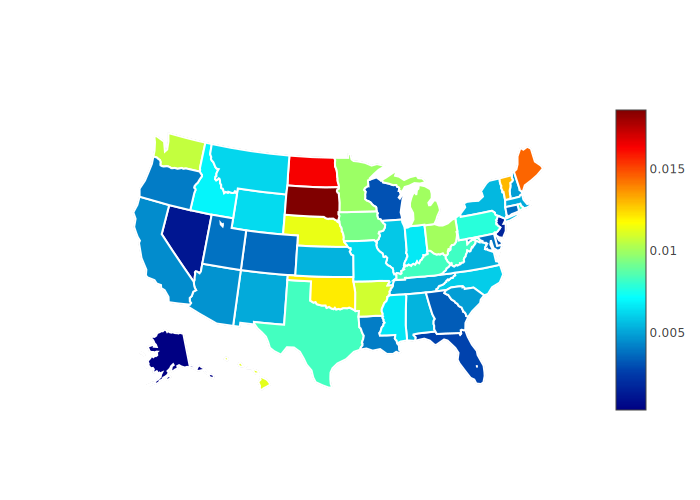
\includegraphics[width=\linewidth]{weather/figs/normalizedfratebyexclweather_ALL_iststorm_statewise_jan11todec17_heatmap}
\caption{
\label{fig:inflatedfrate_tstorm_usmap}
Thunderstorm
}
\end{subfigure}
%
\begin{subfigure}[t]{0.32\linewidth}
\centering
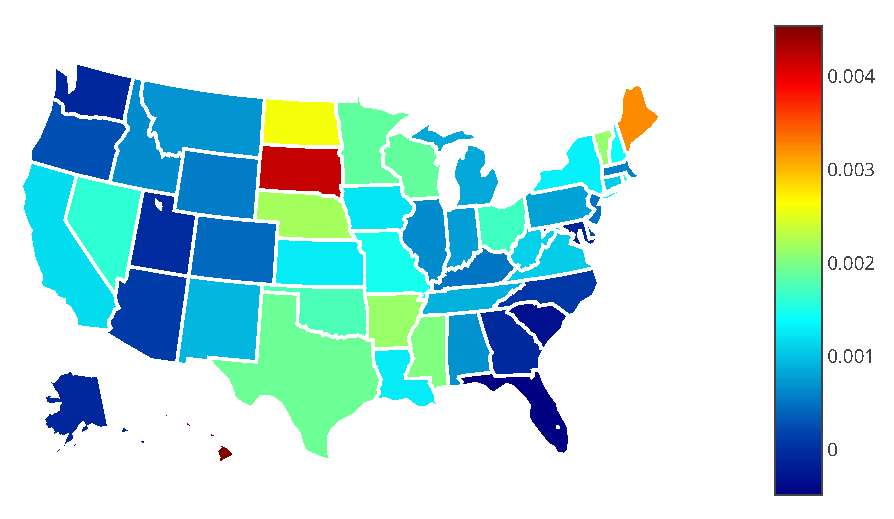
\includegraphics[width=\linewidth]{weather/figs/normalizedfratebyexclweather_ALL_israin_statewise_jan11todec17_heatmap}
\caption{
\label{fig:inflatedfrate_rain_usmap}
	Rain}
\end{subfigure}
%
\begin{subfigure}[t]{0.32\linewidth}
\centering
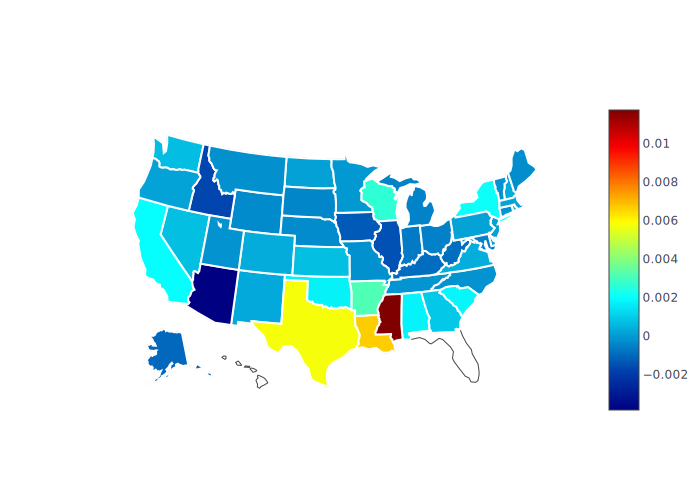
\includegraphics[width=\linewidth]{weather/figs/normalizedfratebyexclweather_ALL_issnow_statewise_jan11todec17_heatmap}
\caption{
\label{fig:inflatedfrate_snow_usmap}
	Snow}
\end{subfigure}
%
\caption{
\label{fig:inflatedfrate_maps}
\figdone
Inflation in hourly dropout probability by U.S.~state for various
	weather conditions.  Large geographic regions can exhibit common
	behavior; northern states are more prone to failures in
	thunderstorms, Midwestern states in rain, and southern states in
	snow.  (Note the different scales for each sub-figure.)}
\end{figure*}
% }}}


Finally, the dropout probabilities of wired link types (cable, DSL, and
fiber) are similar to one another, as are the dropout probabilities of
wireless link types (WISP and satellite), but wired and wireless link
types are different from one another.
%
For example, light rain and light snow have almost no discernible
difference in dropout probabilities for wired links, but light rain
exhibits higher dropout probability for wireless links, and light snow
sees \emph{lower} probability of dropout.
%
Conversely, gale-force winds have a profound increase in dropout
probabilities for wired links, but wireless links are less likely to
drop out during them.
%
It is not surprising that strong winds can cause wired links to fail,
for instance by knocking down above-ground cables.
%
Although wireless links are not affected in the same way, it is
surprising that higher failure rates would not be observed, given that
such strong winds could destroy or blow away satellite dishes.


\paragraph{Summary and ramifications}
%
The results from Figure~\ref{fig:inflatedfrate_by_wtyp_ci_whiskers}
collectively show that different link types can experience weather in
different ways.
%
It is not surprising that different link types would differ in the
\emph{magnitude} with which they experience dropouts; but what we do
find surprising is that some weather conditions (especially snow and
cold) can differ in whether they increase or \emph{decrease} dropout
rates.
%
This has ramifications on network measurement methodology: when
performing outage analysis, it is important to account for both link
type \emph{and} weather condition.
%
%% In the results that follow, we delve deeper into these dropouts by
%% exploring whether dropouts vary across fine-grained measures of wind
%% speed and precipitation, and whether there are geographic influences on
%% weather's effect.




% }}}

\subsection{Geographic variation} % {{{
\label{sec:geography}

Next, we investigate the extent to which different geographic regions
experience weather in different ways.
%
Of course, different states experience different \emph{amounts} of
weather (for instance, we did not observe a statistically significant
amount of snow in Florida).
%
To control for this, we present the inflated probability of hourly
dropouts, comparing hours with a particular weather condition (e.g.,
snow) against all hours without that weather condition.
%
This gives us an apples-to-apples comparison across states, even if
they experience weather conditions in varying amounts.

In Figure~\ref{fig:inflatedfrate_by_state_pcp}, we present the dropout
probability inflation across all 50 U.S.~states (and DC) for three weather
conditions: thunderstorms, rain (excluding hurricanes), and snow.
%
We make two key observations.
%
First, there is a high variation of increased dropout probability across states.
%
For example, during thunderstorms, South Dakota experiences an average
increased hourly dropout probability of 0.018 (3.1 additional
failures per week), while New Jersey increases by only 0.0038 (2.9
additional failures per \emph{month}).
%
Moreover, as shown by the 95\% confidence intervals in the figure,
these differences are statistically significant.
%
We believe this to be an important result because it shows
the role that geography plays in network outages. 


Second, while the raw dropout inflation varies among states, the
relative impact of weather types is common across \emph{most} states:
the increase in dropouts during thunderstorms tends to be greater than
in rain, which in turn tends to be greater than in snow.
%
There are a few notable exceptions.
%
Louisiana and Mississippi have more inflated dropouts in snow than in
thunderstorms, and Florida tends to experience similar amounts of
failures in rain as it does in thunderstorms.
%
By controlling for geography and the total amount of time spent in
weather, this result shows that some weather conditions have more
pronounced impact on dropouts.

Below Figure~\ref{fig:inflatedfrate_by_state_pcp}, we
present a breakdown of the classified link types in each
state, weighted by responsive hours in probing.  The intent
of consulting this graph is to determine whether the outliers
in the top graph are a direct function of the link types  that
are prevalent in a state. North
Dakota has a substantial and exceptional deployment of
Fiber: 50\% of the link-type-classified responsive hours are
from Fiber addresses.  Although our sampling approach is
based on finding 100 addresses in each provider in a region,
and thus is not meant to sample the distribution of link
types used by customers, we note that this is consistent
with published reports that ``60 percent of the households,
including those on farms in far-flung areas, have
fiber''~\cite{csgmidwest}.  Although there are instances where
top and bottom graphs appear related---Vermont (VT) and Maine (ME) show both a
high vulnerability to thunderstorms and a relatively large proportion
of DSL compared to immediate neighbors CT, NH, MA---it appears that
geography is more important than link type at determining the
inflation in probability of dropout in precipitation.




Next, we look beyond individual states to see if there are
\emph{regional} correlations of dropouts.
%
In Figure~\ref{fig:inflatedfrate_maps}, we show maps with the average
inflation in dropout probabilities during thunderstorms, rain
(excluding hurricanes), and snow.


During thunderstorms (Figure~\ref{fig:inflatedfrate_tstorm_usmap}) and
rain (Figure~\ref{fig:inflatedfrate_rain_usmap}) Midwestern states tend
to experience greater inflation of dropouts than other regions.
%
(Maine is an outlier; its dropout inflation during thunderstorm and
rain is due to an abnormally powerful series of storms in
October~2017.)
%
Recall from Figure~\ref{fig:inflatedfrate_by_wtyp_ci_whiskers} that
WISP and satellite links fail more often in thunderstorms and rain than
other link types.
%
One possible explanation for higher dropout rates in the Midwest would
be that these states have more wireless links.
%
This hypothesis is confirmed in
Figure~\ref{fig:inflatedfrate_by_wtyp_ci_whiskers}, which shows that
Midwestern states have more satellite links than other states.


During snow (Figure~\ref{fig:inflatedfrate_snow_usmap}), we see more
pronounced dropout inflation in southern states.\footnote{We do not
include data for Florida or Hawaii, as we did not
observe enough responsive hours of snow to achieve statistical
significance.}
%
Texas, Louisiana, and Mississippi experienced drastically higher
probability of dropouts in snow than in the absence of snow.
%
Unlike rain and thunderstorm, this disparity cannot be explained by
link type alone, as no link types experience drastically higher dropout
rates than others (in fact,
Figure~\ref{fig:inflatedfrate_by_wtyp_ci_whiskers} shows that wireless
links tend to experience \emph{fewer} dropouts during snow).
%
Our insight is that snow seems to affect states where snow is less
common.



% Commonality vs severity plots {{{


% \begin{omitfigure}
% \begin{figure}[t]
% \centering
% \includegraphics[width=\linewidth]{weather/figs/numweatherhours_vs_frate_snow_scatter}
% \caption{
% \label{fig:numweatherhours_vs_frate_snow_scatter}
% P(Dropout) per U.S. state vs. hours of received snow}
% \end{figure}
% \end{omitfigure}

% TODO TODO TODO: Fix this.
\begin{figure}[t]
\centering
\includegraphics[width=0.7\linewidth]{weather/figs/numweathers_vs_frate_snow_scatter}
\caption{
\label{fig:numweathers_vs_frate_snow_scatter}
\figdone
	Hourly dropout probability of hosts (all link types) as a function
	of the number of hours the hosts' nearest U.S.~airport received
	snow (truncated to only those with fewer than 100 hours in snow).
	The less common snow is in a region, the more impact it tends to
	have.}
\end{figure}


% \begin{omitfigure}
% \begin{figure}[t]
% \centering
% \includegraphics[width=\linewidth]{weather/figs/numweathers_vs_frate_rain_scatter}
% \caption{
% \label{fig:numweathers_vs_frate_rain_scatter}
% P(Dropout) per U.S. state vs. proportion of hours of received rain}
% \end{figure}

% \begin{figure}[t]
% \centering
% \includegraphics[width=\linewidth]{weather/figs/numweathers_vs_frate_tstorm_scatter}
% \caption{
% \label{fig:numweathers_vs_frate_tstorm_scatter}
% P(Dropout) per U.S. state vs. proportion of hours of received tstorm}
% \end{figure}
% \end{omitfigure}

% }}}

One possible explanation for the regional effects is therefore that
regions that are less ``familiar'' with a particular weather condition
may be more heavily affected by it.
%
To evaluate this hypothesis, we plot in
Figure~\ref{fig:numweathers_vs_frate_snow_scatter} the hourly dropout
rate of each U.S.~airport as a function of the number of hours each
airport has spent in snow.
%
The results in this figure confirm our hypothesis for snow: the less
familiar a location is to snow, the more often it tends to experience
dropouts.
%
Areas with very small amounts of snow do not experience large
inflation  (ostensibly because there is not enough time for it to
cause damage).
%
Conversely, areas with snow beyond a threshold are more resilient to
snow.
%
A likely reason for this is that regions that are more used to snow
tend to invest more in infrastructure to prepare for and mitigate
it~\cite{state-dots-snow-spending}.
%
We also performed this analysis under thunderstorms and rain (figures
not shown), but did not observe as strong an effect.
%
We hypothesize that this is because all of the airports we measured
experienced enough thunderstorm and rain to grow accustomed to them.

\paragraph{Summary and ramifications}
%
We conclude from these results that different geographic regions can be
affected by weather to varying degrees.
%
We attribute this geographic variation to two leading factors: (1)~the
predominance of some link types over others (e.g., wireless links are
more common in the Midwest), and (2)~how familiar a region is with a
particular weather condition (and thus how prepared for it the region
is).
%
Our results have several interesting ramifications on outage analysis.
%
First, when performing outage analysis, it is important to consider a
representative set of locations and link types; measuring only, say,
cable links would risk overestimating the Midwest's resilience to
dropouts.
%
Second, it is important to note the time and weather conditions when
outage measurements are taken; collecting measurements only during
Spring months\footnote{For instance, in the run-up to the IMC
deadline.}, when thunderstorms are more common, would risk
overestimating dropouts year-round.



% }}}

\subsection{Continuous weather variables} % {{{
\label{sec:continuous}

Thus far in our analysis, we have considered various \emph{binary}
classifications of weather---rain (or not), snow (or not), gale (or
not), and so on.
%
Although these classifications are standard (they are included in the
weather reports we collect), they risk masking the precise effect that
various weather conditions can have.
%
Here, we evaluate dropouts as a function of several \emph{continuous}
weather variables: wind speed, precipitation, and temperature.


Figure~\ref{fig:wind_cont} shows the inflation in the hourly dropout
probability of various link types as a function of wind speed.
%
Note that not all link types share the same values on the $x$-axis;
we aggregate data in increasing values of $x$ until we reach either an
interval of 10 mph or 20 dropout samples (Eq.~(\ref{eq:samples})), whichever comes last.


For all link types, we see almost no inflation in dropout probability
when wind speed is less than 30 mph.
%
Beyond 30 mph, there is little effect on wireless links (WISP and
satellite), but significant increases in dropout probability for wired
links: cable, DSL, and fiber.
%
This is reflected in
Figure~\ref{fig:inflatedfrate_by_wtyp_ci_whiskers}, which showed that
wireless links were not as affected by gale winds.
%
Figure~\ref{fig:wind_cont} expands on this by showing that, as wind speed
increases, dropout inflation increases at a super-linear rate---between
40~mph and 55~mph winds, Cable links' dropout inflation increases by an
hour of magnitude.


In Figure~\ref{fig:temp_cont}, we show dropout inflation as a function
of temperature.
%
Like with wind speed, we bin along the $x$-axis in units of 10, or
20 dropout samples, whichever comes second, and include 95\% confidence
intervals.
%
There are several surprising observations in this figure.
%
First, satellite links are highly sensitive to temperature; at low
temperatures, satellite links are far less likely to experience
dropouts, but this increases steadily, until at approximately
70$^\circ$\,F when satellite links become more likely to fail.
%
Surprisingly, at approximately 80$^\circ$\,F, there is an inflection point at
which satellite links again become significantly more reliable.
%
We hypothesize that there is a confounding factor: satellite links are
less reliable when there is no line-of-sight visibility (e.g., due to
fog), and we suspect that higher temperatures result in less fog.


\begin{figure}[t]
\centering
\includegraphics[width=0.7\linewidth]{weather/figs/inflatedfrateperbinnedval_wind_jan11todec17}
\caption{
\label{fig:wind_cont}
\figdone
Inflation in hourly dropout probability as a function of wind speed
	across multiple link types. All link types experience greater
	dropout probabilities, but satellite and WISP links increase the
	least.  }
\end{figure}

All of the other link types we measured exhibit similar behavior to one
another.
%
They have highly variable dropout probabilities at low temperatures;
they remain mostly steady until 60$^\circ$\,F, then they increase slightly with
higher temperatures.
%
Unlike with our other results, WISPs more closely resemble wired links
than satellite links; we hypothesize that this, too, is because
satellite links are affected by line-of-sight while WISPs and wired
links are not.


Finally, in Figure~\ref{fig:pcp_cont} we measure various link types'
dropout inflation as a function of precipitation in thunderstorms,
rain, and snow.
%
All link types exhibit increased dropout inflation with increased
precipitation, regardless of the overarching weather condition.
%
However, surprisingly, the magnitude of increase varies significantly
across link types.
%
Again, satellite tends to be the most sensitive to change.
%
Other link types are not as consistent across different types of
precipitation; WISP links exhibit nearly the same increase in dropouts
at high thunderstorm precipitation as satellite, but far less during
non-thunderstorm rain.
%
Similarly, DSL links experience a (varying but statistically
significant) increase in dropouts during high snow precipitation, but
not nearly as much during thunderstorm or rain.


There appears to be an inflection point with snow and rain: prior to
0.1~inches of precipitation in rain or snow, non-satellite links
experience little change in their dropout probabilities.
%
After these points, they increase significantly and quickly.
%
Conversely, most links experience (slight but statistically significant)
increases in dropout rates in all levels of precipitation during
thunderstorms.



\paragraph{Summary and ramifications}
%
Weather conditions are often described with binary categories: rain (or
not), snow (or not), and so on.
%
These continuous variable results show that such categories can be
overly coarse; the mere presence of rain or snow does not necessarily
affect most link types, unless there is more than 0.1~inches of
precipitation.
%
Like with our prior results, different link types can exhibit widely
varying behaviors, lending further motivation to incorporate link types
into future outage analyses.


%% Here, we consider continuous weather
%% variables such as rain, temperature, and wind speed.  Each point represents, at
%% some weather condition (x-axis value), how many outage-hours were seen divided
%% by the total number of hours (outage and non-outage) with that weather
%% condition. Where there are not at least 10,000 samples at an x value,
%% subsequent x-axis values are aggregated to determine the probability of failure
%% (y-axis position) and the midpoint between starting and ending x-axis values
%% used to determine the x-axis value.  Points appear for each link type; a line
%% appears for the aggregate of all observations: this line often tracks the DSL
%% points because a majority of our hosts are DSL attached.


% \begin{figure}[t]
% \centering
% \includegraphics[width=\linewidth]{figs/inflatedfrateperbinnedval_pcptstormrain_jan11todec17}
% \caption{
% \label{fig:rain_tstorm_cont}
% Precipitation in rain and thunderstorm}
% \end{figure}

\begin{figure}[t]
\centering
\includegraphics[width=0.7\linewidth]{weather/figs/inflatedfrateperbinnedval_temp_jan11todec17}
\caption{
\label{fig:temp_cont}
\figdone
Inflation in hourly dropout probability as a function of temperature 
	across multiple link types. All link types exhibit non-monotonic
	effects, typically increasing at higher and lower temperatures
	(satellite being a clear exception).
	%whereas most link types experience most failures in very
	% cold or very hot temperatures, 
	% satellite links are most affected in moderate temperatures
	% (70--90$^\circ$~F).
}
\end{figure}

\newlength{\triplefigwidth}
\setlength{\triplefigwidth}{2.3in}
\begin{figure*}[t]
\centering
% \includegraphics[width=\triplefigwidth]{weather/figs/inflatedfrateperbinnedval_pcptstorm_jan11todec17}%
\includegraphics[width=0.32\linewidth]{weather/figs/inflatedfrateperbinnedval_pcptstorm_jan11todec17}%
%
\hfill
%
\includegraphics[width=0.32\linewidth]{weather/figs/inflatedfrateperbinnedval_pcprain_jan11todec17}%
%
\hfill
%
\includegraphics[width=0.32\linewidth]{weather/figs/inflatedfrateperbinnedval_pcpsnow_jan11todec17}
\caption{
\label{fig:pcp_cont} Inflation in hourly dropout probability as a
	function of precipitation during thunderstorm (left), rain
	(center), and snow (right), across multiple link types. All link
	types experience higher dropout probabilities with more
	precipitation, but to widely varying magnitudes. (Note the
	different ranges of the $x$-axes.)}
\end{figure*}


% }}}

%
\chapter{Measuring Residential Internet
  Reliability: a Primer}

\label{cpt:bg}

In this chapter, I provide background and definitions related to the
thesis statement. Then I present related work in measuring Interne
outages in general, and residential Internet outages at the individual
user level in particular. I discuss probing-based techniques to detect
outages remotely in detail and illustrate scenarios where they could
make false inferences about outages. I also illustrate that measuring
Internet reliability using detected outages has nuances and show how
some classes of detected outages need to be treated differently,
depending upon the Internet reliability measure under consideration.

% In this dissertation, I focus
% upon how common outages are and therefore use the \emph{rate} at which
% outages occur. Another metric is the proportion of total measured time detected as outage events.


\section{Background and definitions}

Intuitively, a reliable Internet connection is one that works
continuously. In other words, it experiences no outages. 

Measuring Internet reliability, therefore, necessitates measuring
Internet outages and then using measured outages in a metric that
represents some property of outages. Depending upon the application,
the appropriate outage metric may vary.

The goal of this dissertation is to provide broad, longitudinal, and accurate measurements of
Internet reliability across ISPs, media-types, and geographic
locations in a variety of circumstances. Such measurements can help
users choose from their available Internet options and can inform ISPs
about potential problems in their networks. To achieve this goal, I
propose the following thesis and define terms in the thesis as follows:



\emph{It is possible to remotely and accurately detect substantial outages
  experienced by any device with a stable public IP address that typically
  responds to active probes and use these outages to compare
  reliability across ISPs, media-types and geographical areas.}


\begin{itemize}

\item {\emph{Device with a stable public IP address}: This is a device
    connected to the Internet, like a
home-router, to which an ISP has assigned a public IP address such
that the
assignment is either static, or dynamic in a manner that allows the
duration of dynamic assignment to be estimated.}

\item {\emph{Substantial outage}: I define a substantial outage to be an event where a device
    with an Internet connection is unable to send or receive any
    packets for at least 10 minutes.}

\item {\emph{Accuracy of outage detection}: An outage detection technique is accurate when it
correctly identifies every substantial outage event experienced by an Internet-connected-device, along with its
duration. There are no time-periods when the address
experiences a substantial outage but it goes undetected (false
negatives). Similarly, there are no time-periods classified as
outages when the destination address is able to receive packets from the
Internet (false positives).}

\item {\emph{Reliability}: I define two measures of reliability: one is the raw count of outage
events over measured time and the other is the proportion of total measured time
detected as outage events.} % When estimating a particular ISP's reliability, I
% only use the subset of outages that solely affected that ISP's
% addresses.}
% When estimating the reliability of a geographical area, I
% consider the subset of outages that affected only that geographical
% area.

\end{itemize}

\section{Related work}

The architects of the Internet predicted that network outages could
occur, and designed the Internet to have the ability to route around
outages~\cite{clark-darpa}. As predicted, a variety of factors cause
outages in the Internet, including optical fiber
cuts~\cite{fiber-cuts}, routing and infrastructure
failures~\cite{backbone-failures-1999, ratulbgp}, and
hurricanes~\cite{pingin}.

%TODO: Cite ratulbgp somewhere, network-black-holes, feamster:sigmetrics:failures

Large Internet outages that can affect packets from thousands of
Internet hosts have received attention from the research
community~\cite{censorship-outages, trinocular, hubble, paxson-e2e,
hubble, netdiagnoser, lifeguard, poiroot,
phillipa-outages-mailing-list, california-fault-lines,
delayed-routing-convergence, consensus-routing, routing-e2e-path-perf,
voip-bgp-convergence}. Outages occurring in the Internet's core can
cause Internet path failures; researchers have investigated transient
Internet path failures caused by route
changes~\cite{delayed-routing-convergence, consensus-routing,
routing-e2e-path-perf, voip-bgp-convergence} and longer path failures
caused by infrastructure device outages~\cite{paxson-e2e, hubble,
netdiagnoser, lifeguard, poiroot, phillipa-outages-mailing-list,
california-fault-lines}. Dainotti et~al.~\cite{dainotti-imc11} observe
Internet Background Radiation traffic sent to IPv4 darknets to detect
outages affecting entire countries.

% Other studies detect outages at the
% country-level~\cite{censorship-outages} and at the network prefix
% level~\cite{trinocular, hubble}.

Another class of techniques detects outages at the Internet's edge,
for network prefixes or address blocks, but
does not target outages of individual users' Internet
connections. Hubble studies reachability problems affecting BGP
prefixes~\cite{hubble}. Trinocular detects outages affecting /24
address blocks. Richter
et~al.~\cite{advancing-outage-art} use the observation point of a
large CDN to detect periods of reduced activity from /24 address
blocks consistent with outages. CAIDA's IODA
system~\cite{ioda-project-page} detects outages affecting countries, ASNs, and geographic provinces using three complementary
datasets: BGP updates from Routviews~\cite{routeviews} and RIPE RIS~\cite{ripe-ris}, active probing data
obtained with CAIDA's implementation of the Trinocular methodology,
and IBR data using the technique introduced by Dainotti et~al.~\cite{dainotti-imc11}. 


 % Industry provides some options to
% study failures but they either focus solely on websites that are
% down~\cite{downdetector, outageanalyzer, isitdownrightnow, downforeveryoneorjustme}, or offer services to monitor
% large customer networks~\cite{thousandeyes}. 
However, outages that affect individual users have received comparatively less
attention~\cite{pingin, grover2013peeking, disco, alwayson}. In the rest of this
section, I classify these efforts to detect outages into on-premises
outage detection techniques and remote probing-based outage detection
techniques, and
discuss their approaches and challenges in detail.

% Why do I care only about complete outages and not partial ones?
% Because they are easy to define! :P
% Because they are more likely to be last-mile link. Aha! Yes, so a
% complete outage means we will have the ability to isolate the fault

% We define a link to experience an outage when it experiences peformance
% degradation resulting in unusually high loss and/or delay. When a link
% experiences delay but no loss, we define that link to be \emph{sleepy}
% and we refer to the event as a \emph{sleep}. When a link experiences
% loss but no delay, we define that link to be \emph{lossy} and we refer
% to the event as a loss. When a link experiences complete loss, i.e.,
% all packets on that link are dropped, we define that link to be
% \emph{out} and we refer to the event as an \emph{outage}. Note that by
% definition, every \emph{outage} event is also a \emph{loss}
% event. When a link experiences delay and loss, we define that link to
% be \emph{sleepy-lossy} and we refer to the event as a
% \emph{sleep-loss}. When we speak of a single probe being lost/delayed,
% we will refer to it a \emph{probe-loss} /\emph{probe-sleep}.



% Several studies have tried to detect outages. 

% Find which ones study outages using passive techniques?

% Find which ones study outages at not the last-mile

% Find which ones study outages at the last-mile but using dedicated
% hardware (Ark, RIPE Atlas)

\subsection{On-premises outage detection techniques}
% The redundancy present in the core of the Internet is
% mostly absent in residential networks, owing to the high cost of
% deploying redundant last mile links. Even multihomed last mile links for business connectivity
% often share the same upstream hardware, representing a single point of 
% failure. Residential link failures directly impact end-users and as a result,
% are of interest to service providers, policy makers, and the end-users themselves.

% Most residential end-users today lack the means to understand the
% reliability of their Internet connectivity over time, and of comparing
% reliability across competing ISPs. They have to rely upon speedtest
% tools which can offer estimates of connectivity over a few seconds but
% not over longer timescales. 
Recognizing the need for long term measurements of residential
Internet performance, policymakers such as the FCC from the U.S., and
Ofcom from the U.K. have deployed the SamKnows hardware
platform~\cite{samknows} inside residences to measure residential
Internet connections continuously by performing active and passive
measurements and reporting their results to users, ISPs, and policy
makers. RIPE NCC, the European RIR, has pioneered the RIPE
Atlas~\cite{atlas} project and Sundaresan et al. the BISmark
project~\cite{bismark-main-bib}, which also study user connectivity
using dedicated hardware measurement devices on user
premises. On-premises techniques can also use measurements from
software deployed on user machines: the DIMES project~\cite{netdimes}
and DASU are two notable examples~\cite{Dasu:NSDI2013}.

% TODO: I don't like the "as done in the DIMES project" above.

% I mention this later, so no need to talk about it now. 
% ; however, this approach
% is not well suited to detecting outages since the DIMES software is
% often installed on laptops~\cite{dhcp-dimes}.

% To
% offset some of the scalability costs, on-premises outage detection systems can also be software-based 

% TODO: Consider if any of these techniques needs to be described in
% additional detail
% Disco~\cite{disco} uses Kleinberg's burst detection to detect
% events where many RIPE Atlas probes disconnect from
% their infrastructure in a correlated manner.


% In essence,
% they are also probe-based outage detection techniques, in that the
% absence of any probes indicates an outage; however, they are
% on-premises and not remote.
Hardware-based approaches can offer accurate reports about
Internet connectivity since the hardware devices are designed to make
measurements continuously as long as they are powered. These techniques have the
ability to perform a range of other measurements such as DNS anycast
tests that can identify which instance of a root-server is closest,
and even passive measurement of the websites that users
access. However, these approaches are fundamentally limited in scale
since their hardware is expensive, distributing the hardware to users
is time consuming, and convincing users to keep their hardware running
is challenging. For example, the RIPE Atlas project, which began in
2010 and has been continuously expanding across the world, has fewer than 10,000 probes that are currently making measurements, out
of more than 15,000 distributed probes.

While some of these costs can be offset by utilizing measurements from
deployed software on user systems~\cite{netdimes, dhcp-dimes, Dasu:NSDI2013} or using a combination of hardware
and software measurements~\cite{IMC2014-Broadband-bischof}, deploying software widely remains
challenging. Separating user behavior, such as turning off their laptops, from
Internet outage events presents additional challenges for these techniques~\cite{dhcp-dimes}.
 
\subsection{Probing-based remote outage detection techniques}

% TODO: Talk about Zmap. It cannot do adaptive probing, being
% stateless, and hence cannot be used for individual outage detection.

Probing-based remote outage detection techniques can detect
connectivity problems remotely through active probing from servers
under reseacher control. Though this approach will prevent 
certain types of measurements, such as DNS anycast tests, it can measure
Internet connectivity for individual users at scale. However,
existing techniques can infer false outages in some scenarios as I
illustrate next.

Probing-based remote outage detection techniques study connectivity problems by
sending active probes (such as ping's echo requests) and use probe
responses to infer connectivity problems. For example, an
echo-response from the end-host indicates that its network connection
is working. If a previously responsive destination ceases to respond
to probes, current techniques infer that the destination could be
experiencing connectivity problems. Thunderping~\cite{pingin},
Trinocular~\cite{trinocular}, and Zmap~\cite{durumeric2013zmap}, have
used this technique to detect outages, albeit at different scales. I
discuss each approach in detail next.

\subsubsection{Trinocular detects failures of /24 address blocks}

Trinocular pings addresses in ~4M /24 address blocks and
uses the responses to detect Internet outages affecting entire blocks. Using historical
data from the ISI census~\cite{census-survey}, it models the responsiveness of
blocks and finds subsets of addresses within each block that are
likely to respond to pings. The system pings a few of these addresses
from each block at random and probes them in 11-minute
rounds. Trinocular then employs Bayesian inference to reason about
responses from blocks. When a block's responsiveness is lower than
expected, Trinocular probes the block at a faster rate and eventually
detects an outage when the follow-up probes also indicate the block's
lack of Internet connectivity.

\subsubsection{Thunderping detects failures of individual addresses
  during severe weather}

Thunderping pings
sampled addresses from multiple ISPs in geographic areas in the United
States. Originally designed to evaluate how weather affects Internet
outages, the system uses Planetlab vantage points to ping 100 IPv4
addresses from multiple ISPs in U.S. counties with active
weather alerts. Each address is pinged from multiple Planetlab vantage
points (at least 3) every 11 minutes, and addresses in a county are
pinged six hours before, during, and after a weather alert for that
county. 


\subsubsection{Zmap was used to study Internet outages during
  Hurricane Sandy}

Zmap is an active probing technique designed to send packets of a
specified type (such as ICMP echo) to all IPv4 addresses at
very fast speeds (under an hour in 2013~\cite{durumeric2013zmap},
under 5 minutes today~\cite{zippier-zmap}. A key to these speeds is that the
Zmap tool chooses to not store state at the prober; instead, response
packets are matched with sent ones by encoding destination-specific data
in the sent packets. By using cyclic generators, Zmap probes
destination addresses in a random order, reducing probing burden on
individual ISPs. However, Zmap's decision to not store state comes
with a trade off: probe retransmissions upon the detection of a lost
probe is difficult. The Zmap
tool was used to detect Internet outages during Hurricane
Sandy~\cite{durumeric2013zmap}. % However, finding smaller Internet failure
% events with the Zmap tool is challenging.

% Since outages are infrequent and can affect small parts of
% the address space, finding them would require running repeated Zmap
% scans of the entire address space on the order of minutes. Even if this is technically feasible,
% it remains an open problem whether such an aggressive probing scheme
% is warranted.

% The following was from related work in corrfails, don't thin it's
% necessary here.
% The key difference of this work from Trinocular is that we do not assume
% that correlated failures span entire /24-address blocks; instead, we
% look for correlated failures of addresses related by geography and
% ISP. While we share Trinocular's intuiton that dependent events will
% affect related addresses, Trinocular's notion of relatedness is solely
% that of belonging to the same /24. With the IPv4 address space
% breaking up, we hypothesized that addresses in disparate /24s may be
% affected by a correlated failure event. Further, a power outage may
% affect a few addresses but from several different ISPs.

% TODO: I probably don't need this part about scaling at all. 
% \subsubsection{Can scale, but not indefinitely}

% While probing-based outage detection techniques can scale to probing hundreds
% of thousands of addresses, they cannot scale indefinitely. Very high
% probe volume can cause traffic to be viewed as malicious and can
% result in probes getting blacklisted and in abuse
% reports~\cite{durumeric2013zmap}. Further, high probe volume increases
% the state that needs to be stored by the prober. While probing
% schemes like Zmap have circumvented this problem by not storing
% state~\cite{durumeric2013zmap}, adaptive retransmission to confirm a
% suspected outage requires the storage of state.

% Trinocular is an outage detection system that employs active
% probes to detect outages for entire /24 prefixes. It uses historical
% measurements to 

% Thunderping~\cite{pingin}, detects last-mile
% link outages for individual residential links during times of predicted severe weather
% conditions using pings, and correlates outages with weather
% conditions. The US National Weather service issues severe weather alerts for areas that are
% likely to experience conditions of severe weather; Thunderping uses
% these alerts to select geographic areas to study. Using
% Maxmind, a popular geolocation service, it then finds IP addresses in
% these geographic areas and pings these addresses from multiplee
% PlanetLab vantage points before, during, and after the weather
% event. We use the results of these pings to infer outages
% and correlate them with observed weather conditions to measure
% the effect of weather upon residential Internet connectivity.


% \begin{figure}[tb]
% % \centering
% \begin{center}
% \includegraphics[width=3in]{figs/pingin_real_deal_v13}
% \end{center}
% \caption{\label{fig:thunderping} Thunderping detects outages in
%   last-mile links during times of predicted severe weather. It uses
%   weather alerts from NOAA to find areas that are likely to be
%   affected by severe weather. It then pings IP addresses in those
%   areas before, during and after the weather alerts from multiple
%   PlanetLab vantage points and uses the
%   results to infer outages.}
% \end{figure}

% \subsubsection{Improving the accuracy of remote probing based outage
%   detection techniques}

% Can measure reliability inaccurately
\section{Probing-based remote outage detection techniques can
be inaccurate}

% I define a probed destination address to undergo an ``outage'' event
% when the address is unable to send or receive any Internet packets. The ideal outage detection technique should be capable of
% identifying every outage event, along with its
% duration. There should be no time-periods when the destination address
% experiences an outage but the outage is undetected (false
% negatives). Also, there should be no time-periods classified as
% outages when the destination address is able to receive packets from the
% Internet (false positives).

Probing-based remote outage detection techniques can infer false
negative and false positive outages as a consequence of their foundational
assumption: that a response to an active probe indicates a working path to the probed
IP address and that lack of response is indicative of
failure. False negatives can occur when the probe rate
to a destination address is low, so that very short outages
experienced by the address go undetected. For example, with
Thunderping's probing scheme of sending a ping every 11 minutes from
each of its vantage points to a destination address~\cite{pingin}, it is possible that an outage lasting
shorter than 11 minutes is not observed by each vantage
point. Increasing the probe rate can limit the maximum duration
of these false negative outages; remote probing based outage detection
techniques must tradeoff the rate
with which they probe a given destination and the duration of the
longest outage that they can fail to detect. 

While false negative outages can be controlled by probing faster,
false positive outages pose a potentially larger accuracy problem. Current
techniques can make false positive inferences about
outages in the following scenarios:

% \begin{itemize}

% \item{\bf{Confusing delay with loss:}}

\subsection{Confusing delay with loss}

Traditionally, active probe based approaches time out probes after a
few seconds. Thunderping~\cite{pingin} and
Trinocular~\cite{trinocular} time out probes after a few
seconds. Responses that arrive after the timeout will be reported as
lost. When this happens, existing techniques would infer loss though
the responses are in fact merely delayed. Chapter~\ref{cpt:timeouts}
presents a measurement study on probe response latencies in networks
around the world and discusses approaches to disambiguate delayed
probes from lost probes.

% TODO: Raise whether extreme delay is an outage.

\subsection{Making false inferences about outages due to dynamic
      addressing}
% \item{\bf{Making false inferences about outages due to dynamic
%       addressing:}}

 Consider an IP address that was previously responsive. If the host
to which that IP address was assigned changed its IP address as a
result of dynamic addressing, and if the probed IP address is not
reassigned to any host, then echo responses will cease to
arrive. Existing techniques would thus infer false probe-loss and
consequently, false outages. Consider an alternate scenario where the
probed IP address has an outage. Suppose that at some point during the
outage, the IP address is reassigned to some other end-host which
responds to probes. Existing techniques would infer that the arrival
of responses signals the end of the outage and would infer that the
outage ended prematurely.  I address how to mitigate false inferences
due to dynamic address reassignment in Chapter~\ref{cpt:addr_change}.

% \item{\bf{Some outages can falsely lower inferred reliability}}
% When analyzing ISP-level or media-type-level reliability, our
% reliability inferences for an ISP should only be based upon outages that
% affected solely that ISP's customers. However, power outages and
% undersea cable cuts can result in outages to many ISPs'
% customers. Also, users sometimes choose to voluntarily shut down their home Internet
% equipment~\cite{grover2013peeking}. If a probing-based remote outage detection technique happens to
% measure an address during these times, probes sent to that address
% will cease to arrive, leading to the inference of an outage. When
% measuring ISP-level or media-type-level reliability, these outages
% must be filtered.

% \end{itemize}

% the rest of the proposal.
 % false probe-loss inference due to early timeout in
% Section~\ref{sec:timeouts} and false probe-loss inference due to IP
% address change in Section~\ref{sec:addr_change}.

\section{Analyzing Internet reliability using detected outages}
% depending upon the question under investigation

Internet reliability can be measured along several dimensions,
depending upon the application. For example, users who require the
Internet for work, or who use health monitoring equipment that needs a
continuously working Internet connection~\cite{ideal-life,
remote-health-elderly}, may be interested in finding which ISP and
media-type in their area provides the most reliable Internet
connection. A per-ISP or per-media-type reliability metric would be
appropriate for this application since these metrics can facilitate
comparisons.

Another application of Internet reliability could be the
identification of geographic regions and challenging conditions with
particularly poor connectivity. A per-region reliability metric could
allow policymakers and ISPs to identify problematic areas and drive
Internet infrastructure deployment in such areas.

Reliability can also be measured along various combinations of ISP,
media-type, geographic region, and challenging conditions. Such
measures can help find the most reliable ISP and media-type for a
geographic region that is particularly susceptible to a challenging
weather condition (such as blizzards, for example). Important
infrastucture in those areas can then use the most reliable ISP and
media-type combination.

\subsection{Not all outages are relevant to Internet reliability
measures}

Even after mitigating errors in outage inferences due to high latency
and dynamic address reassignment, some false outages may
remain. 

Additionally, the set of detected outages that should be considered in
reliability metrics can vary depending upon the application. Here are
three potential applications with different requirements:

\begin{itemize}

\item{Suppose the goal is to measure the effectiveness of broadcasting
    critical information (such as severe weather alerts or Amber
    alerts) over the Internet. An Internet reliability metric, such as
    the rate of Internet outages over time, offers a sense of how many
    users in each ISP or geographic region can be reached through such
    a broadcast. For this application, all Internet
    outages---including outages due to users turning off their home
    Internet equipment---should be represented in the metric. }

\item {When comparing Internet reliability across geographic regions,
    perhaps to identify areas with particularly poor connectivity, outages due to
    user behavior should not be considered in the reliability
    metric. Grover et al. report that users sometimes voluntarily
    power off their home Internet
    equipment~\cite{grover2013peeking}. Probing-based techniques would
  detect such instances as Internet outages since a previously
  responsive address ceases to respond to probes. Without accounting
  for such outages, we may overestimate the outage rate in a region.}
 
\item {When comparing reliability across ISPs, the reliability metric
should ideally only consider outages that each ISP was responsible
for. Doing so ensures that ISPs offering services in challenged areas
do not have their reliability lowered by events such as power outages
or user behavior.}

\end{itemize}

\subsection{Estimating how a challenging condition affects Internet
  reliability}

Suppose we wish to assess the effect of a challenging condition or environment---like
the presence of a thunderstorm---upon the Internet reliability of a
group of addresses. This group of addresses could be a set of
addresses that share some relationship to each other: they could
belong to the same ISP, media-type, geographic region etc. Such an
assessment would help identify areas and networks that are
particularly prone to Internet connectivity problems in certain types
of weather. Chapter~\ref{cpt:weather} describes how to perform these assessments.

\subsection{Categorizing outages by their potential cause}

Since the set of detected outages that should go into a reliability
metric varies by application, depending upon the outage's cause, there
is a need to classify detected outages. Chapter~\ref{cpt:corrfails}
discusses a technique that uses simultaneous failures of related
addresses to achieve this classification.

\section{Conclusions}

Using a seven year dataset collected by probing residential IP addresses in the U.S., I showed that a variety of weather conditions can inflate the likelihood of Internet dropouts. I quantified this inflation and show that it varies depending upon the type of weather, link type, and geographic location. 
% We also showed that the time to recover from a dropout increases during weather events.

Even ignoring times when hurricanes were active, all link types see more failures during thunderstorms---fiber addresses, the most resilient to thunderstorms still observed an additional dropout every 11 days, while satellite addresses, the most susceptible, observed an additional dropout every day. High wind speeds result in a super-linear increase in dropout probability for wired links while higher precipitation results in particularly pronounced increases in dropout probability for wireless links.

The extent to which weather conditions can inflate the probability of dropouts varies considerably with geography. States in the Midwest are susceptible to dropouts during rain while states in the south experience dropouts much more often in the snow: addresses in Mississippi, for example, experience an additional dropout every 4 days. 

The reliability analyses in this chapter were performed using dropouts of individual IP addresses. Although dynamic addressing and user behavior also constitute dropouts, the key observation that allowed the use of dropouts for reliability comparisons is that the inflation in dropout rates during the occurrence of severe weather conditions is due to the additional outages that occur. Confounding factors such as dynamic addressing and user behavior do not positively correlate with peak diurnal failure periods; therefore, the increase in dropout rate during a weather condition is equivalent to the increase in outage rate during that condition. 


\chapter{The need for measuring individual address outages}
\label{cpt:corrfails}

In this chapter, I develop and evaluate an approach to detect
dependent \emph{Internet disruption} events that affect multiple residential
addresses simultaneously using measurements of individual address disruptions
gathered with the Thunderping technique. Borrowing terminology from
Richter et al.~\cite{advancing-outage-art}, I define an Internet
disruption event for an address to be the abrupt loss of response to active probing
from that address.

% I define a dependent Internet disruption event to be one which affects
% multiple customers due to a shared underlying cause (such as a network
% or power outage). My insight is that such events can affect multiple
% addresses that are related to each other simultaneously.
Techniques that detect outages at the Internet's edge often seek
disruption events affecting a substantial set of addresses. The set of addresses may comprise
those belonging to the same /24
address block~\cite{trinocular,advancing-outage-art}, BGP
prefix~\cite{hubble}, or country~\cite{dainotti-imc11}.  
Techniques seek such disruption events because individually, each large disruption has
impact and their size makes them easier to confirm, e.g., with operators. In contrast, disruptions
affecting only a few users are harder to detect with confidence.  For example, the
lack of response from a single address might best be explained by a
user switching off their home router---hardly an outage.
However, residential Internet
outages may be limited to a small neighborhood or apartment block; prior
techniques are likely to miss such events.

% In the rest of the chapter, I describe work with colleagues where we
% use a novel approach based upon Binomial hypothesis testing to
% detect instances of per-address disruption events that are unlikely to
% have happened independently and flag these as dependent Internet
% disruption events. Next, we characterize these dependent disruption
% events and present results that challenge conventional wisdom on how
% such disruptions affect Internet address blocks. We show that many of
% these events would be missed by existing techniques that do not
% perform individual address outage detection.

In the rest of this chapter, I describe work with colleagues where we
demonstrate a technique that detects disruption events with
quantifiable confidence, by investigating the potential dependence
between disruptions of multiple IP addresses in a principled way. We
apply a simple statistical method to a large dataset of active probing
measurements towards residential Internet users in the US. We find
times when multiple addresses experience a disruption simultaneously
such that they are unlikely to have occurred independently; we call
the occurrence of such events \emph{dependent disruptions}. We
characterize these dependent disruption events and present results
that challenge conventional wisdom on how such disruptions affect
Internet address blocks. We show that many of these events would be
missed by existing techniques that do not perform individual address
outage detection.

% begin by providing background on why residential
% reliability measurements could require measurements of individual
% addresses' outages. 

\section{Background: dependent residential outages can be small}

Residential Internet connections are vulnerable. The last-mile link
connecting home routers to their ISP is typically not multi-homed and
is therefore a single point of failure. Further, last-mile links can
be damaged by exposure to the elements or by broken tree limbs blown
by the wind. Thus, residential outages may be limited to a small
neighborhood or apartment block.




\section{Conclusion and future work}

In this dissertation, I described how to measure residential Internet
reliability remotely using probing-based techniques. These techni

First, I showed
how to detect Internet outages accurately using these techniques by
analyzing and mitigating potential scenarios that can cause these
techniques to make false inferences about detected outages. 

 can measure Internet
reliability for individual users broadly, longitudinally, and
accurately. In spite of their potential, these techniques can make
false inferences about outages in two scenarios: when probe
responses are delayed beyond timeouts and when addresses get dynamically
reassigned. I described preliminary work which studied how commonly
probes are delayed beyond responses and described measurements of
dynamic addressing across the world that can help build a model of
dynamic addressing. For each outlined scenario, I proposed approaches
that can mitigate false outage inferences when that scenario
occurs. Finally, I discussed an approach to segregate outages into
categories that suggest cause, and how we can use these categorized
outages to study Internet reliability along different dimensions.


\clearpage % TODO: Find out what clearpage does?
\bibliographystyle{plain}
\bibliography{longnames,outages}

\end{document}
